
\documentclass[doublespacing]{brandeis}
\usepackage{bm}
\usepackage{url}
\usepackage{tikz}
\usepackage{soul}
\usepackage{color}
\usepackage{times}
\usepackage{dsfont}
\usepackage{pifont}
%\usepackage{breqn}
\usepackage{textcomp}
\usepackage{wrapfig}
\usepackage{graphicx}
\usepackage{multirow}
\usepackage{multicol}
\usepackage{footnote}
\usepackage{pgfplots}
\usepackage{verbatim}
\usepackage{textcomp}
\usepackage{booktabs}
\usepackage{textcomp}
\usepackage{paralist}
\usepackage{algorithm}
\usepackage{algpseudocode}
\usepackage[makeroom]{cancel}
\algrenewcommand\textproc{} % to change function names to lower case
\usepackage{microtype}
\usepackage{mathrsfs}
\usepackage{schemabloc}
\usepackage[final]{pdfpages}
\usepackage{algpseudocode}
\usepackage[export]{adjustbox}
% Optional: If your LaTeX has microtype, use it to improve text quality:
%\usepackage{microtype}
\usepackage[most]{tcolorbox}
\usepackage{booktabs,tabularx}
\usepackage{caption}
\captionsetup[table]{skip=4pt,singlelinecheck=off}

% correct bad hyphenation here
\hyphenation{op-tical net-works semi-conduc-tor}

% Recommended: If your dissertation contains math, use the AMS packages:
\usepackage{amsmath}
\numberwithin{equation}{section}
\usepackage{amssymb,amsthm}
\usepackage[caption=false,font=normalsize,labelfont=sf,textfont=sf]{subfig}
%
\let\proof\relax
\let\endproof\relax
\usepackage[final]{pdfpages}


%\addtolength{\textfloatsep}{-5mm}
\addtolength{\textfloatsep}{-3mm}
\pgfplotsset{compat=1.5}

% Required: To satisfy UTD's formatting requirements for citations, use the
% "natbib" package.  (Use other citation packages at your own risk; not all
% are flexible enough to meet UTD's requirements.)  If you wish to use numeric
% citations, change "authoryear" to "numbers" below.  Use the "chicago" BibTeX
% style, which most closely matches the Turabian formatting required by UTD.
% UTD mandates a blank line between each pair of bibliography entries, so set
% \bibsep as shown below.  Finally, if you are accustomed to using \cite as
% your citation macro, point it to natbib's \citep macro as shown.
\usepackage[authoryear, sort]{natbib}
\bibliographystyle{chicago}
\setlength{\bibsep}{12pt plus 1pt minus 1pt}
\let\cite=\citep
\usepackage{rotating}
%\theoremstyle{remark}

\theoremstyle{definition}
\newtheorem{definition}{Definition}[]
%\newtheorem{theorem}{Theorem}[]
\newtheorem{example}{Example}
\newtheorem{homework}{Homework}
%\usepackage[pagebackref=true,breaklinks=true,bookmarks=true]{hyperref}
\usepackage[pagebackref=true,breaklinks=true,colorlinks=true, citecolor=green,linkcolor=light-blue,urlcolor=blue,bookmarks=true]{hyperref}
%%% End of packages.
% Define all your personal macros here (if you have any).
%
\definecolor{light-blue}{rgb}{0.30,0.35,1}
\definecolor{light-green}{rgb}{0.20,0.49,.85}
\definecolor{purple}{rgb}{0.70,0.69,.2}

\newcommand{\lb}[1]{\textcolor{light-blue}{#1}}
\newcommand{\bl}[1]{\textcolor{blue}{#1}}

\newcommand{\maybe}[1]{\textcolor{gray}{\textbf{MAYBE: }{#1}}}
\newcommand{\inspect}[1]{\textcolor{cyan}{\textbf{CHECK THIS: }{#1}}}
\newcommand{\more}[1]{\textcolor{red}{\textbf{MORE: }{#1}}}

% FYA
\newcommand{\cmt}[1]{{\footnotesize\textcolor{red}{#1}}}%{#2}
%\newcommand{\note}[1]{\cmt{Note: #1}}
%\newcommand{\todo}[1]{\textcolor{cyan}{TO-DO: #1}}
\newcommand{\review}[1]{\noindent\textcolor{red}{$\rightarrow$ #1}}
\newcommand{\response}[1]{\noindent{#1}}
\newcommand{\stopped}[1]{\color{red}STOPPED HERE #1\hrulefill}

%Text commands
\newcounter{mnote}
\newcommand{\marginote}[1]{\addtocounter{mnote}{1}\marginpar{\themnote. \scriptsize #1}}
\setcounter{mnote}{0}
% \newcommand{\comment}[1]{}
\newcommand{\ie}{$i.e.$\ }
\newcommand{\eg}{e.g.\ }
\newcommand{\cf}{c.f.\ }
\newcommand{\yes}{\checkmark}
\newcommand{\no}{\ding{55}}

%Reference commands
\newcommand{\flabel}[1]{\label{fig:#1}}
\newcommand{\seclabel}[1]{\label{sec:#1}}
\newcommand{\tlabel}[1]{\label{tab:#1}}
\newcommand{\elabel}[1]{\label{eq:#1}}
\newcommand{\alabel}[1]{\label{alg:#1}}
\newcommand{\fref}[1]{\cref{fig:#1}}
\newcommand{\sref}[1]{\cref{sec:#1}}
\newcommand{\tref}[1]{\cref{tab:#1}}
\newcommand{\eref}[1]{\cref{eq:#1}}
\newcommand{\aref}[1]{\cref{alg:#1}}

\newcommand{\bull}[1]{$\bullet$ #1}
\newcommand{\argmax}{\text{argmax}}
\newcommand{\argmin}{\text{argmin}}
\newcommand{\mc}[1]{\mathcal{#1}}
\newcommand{\bb}[1]{\mathbb{#1}}


\def\tidx{t}
%\def\comment
%\def\value{V}
% from https://www.cs.jhu.edu/~jason/advice/write-the-paper-first.html
\newcommand{\Note}[1]{}
\renewcommand{\Note}[1]{\hl{[#1]}}  % comment out this definition to suppress all Notes
%\algnewcommand\algorithmicforeach{\textbf{for each}}
%\algdef{S}[FOR]{Foreach}[1]{\algorithmicforeach\ #1\ \algorithmicdo} %

%\newcolumntype{M}[1]{>{\centering\arraybackslash}m{#1}}
\def\coriolis{\textbf{\textit{C}}}
\def\massinertia{\textbf{\textit{M}}}
\def\torque{\bm{\tau}}
\def\frictionvec{\textbf{\textit{f}}}
\def\Smat{\textbf{\textit{S}}}
\def\Bmat{\textbf{\textit{B}}}
\def\wheelrad{\textbf{\textit{r}}}

\def\stateweight{\textbf{\textit{w}}_x}
\def\actionweight{\textbf{\textit{w}}_u}
\def\advactionweight{\textbf{\textit{w}}_v}

%Thesis defs
%\def\upchi{\textchi}
\def\kau{\mc{K}}
\def\particle{\bm{x}}
\def\deformationgrad{\textbf{F}}
\def\refconf{\bm{\upchi}_0}
\def\refconfbody{\mathscr{B}_0}
\def\conf{\bm{\upchi}}
\def\currconf{\bm{\upchi}}
\def\Eulerian{\mc{E}}
\def\cauchystress{\bm{\sigma}}
\def\stresscomp{\sigma}
\def\currconfbody{\mathscr{B}}
\def\materialresponse{\textbf{G}}
\def\orthoggroup{{\textit{SO}}(3)}
\def\liegroup{{\textit{SE}}(3)}
\def\liealgebra{\mathfrak{se}(3)}
\def\identity{\textbf{I}}
\newcommand{\trace}[1]{\textbf{tr}(#1)}
\def\leftcauchy{\textbf{B}}
\def\rightcauchy{\textbf{C}}
\def\fiber{\textbf{dx}}

\def\dof{\text{DOF }}
\def\dofs{\text{DOFs }}
\def\reline{\mathbb{R}}
\def\curve{\deformationgrad}
\def\twist{{\xi}}
\def\contactforce{\tilde{F}}
\def\contactforcecomp{f}
\def\gaussianmap{\textbf{}n}
\def\contacttorquecomp{\tau}
\def\wrt{with respect to }
\def\curveparam{\position}
\def\basis{\bm{e}}
\def\pose{{g}}
\def\selmap{{B}}
\def\manipmap{{G}}
\def\jacob{\bm{J}}
\def\normal{\bm{n}}
\def\position{\textbf{r}}
\def\deformationgradcur{\textbf{H}}
\def\eulerianvel{\textbf{v}(\position, t)}
\def\headparam{\zeta}
\def\strain{\mathrm{\Psi}}
\def\strainiso{\mathrm{\Psi_{\text{iso}}}}
\def\strainfiber{\mathrm{\Psi_{\text{mesh}}}}

% mechanism defs
\def\wallthickness{1cm}
\def\sorodiam{9 cm}
\def\sorodiamdim{5-6.25cm}

% inline macros
\newcommand{\putsoro}[2]{\includegraphics[width=.45\columnwidth,height=#2\columnwidth]{../../../PhDThesis/figures/#1}}
\newcommand{\sorowidth}{.35}


%\newtheorem{theorem}{Theorem}[]
%\newtheorem{example}{Example}
%\newtheorem{homework}{Homework}

\providecommand{\hyperref}[2][]{#2}

\newenvironment{exampleclasscode}
{\parindent=1cm\vskip0pt plus2pt minus0pt\begin{verse}}
	{\end{verse}\vskip0pt plus2pt minus0pt}
%
%%% End of personal macro definitions.
%%% The following definitions MUST come before the document begins.
%
\author{RBOT250: Robot Motion Planning, Manipulation and Control \\
	Instructor: Dr. Olalekan Ogunmolu}
\title{RBOT 250: Robot Manipulation, Planning, and Control.
}

\pdfoutput=1    % for arxiv tex processor
\begin{document}	
	\frontmatter
	
	%\signaturepage
	\copyrightpage{2020} % optional
	
	\tableofcontents
	\listoffigures % required if you have any figures
	\listoftables % required if you have any tables
	
	\mainmatter
%%
%\authorrunning{Lekan Molu} 
%
%\institute{
%	Graduate Professional Studies \\
%	Rabb School of Continuing Studies \\
%	Brandeis University}


%\titlerunning{RBOT 250}
%\maketitle              % typeset the title of the contribution

\newpage
\chapter{Preamble}
\label{chap:intro}

Consider this your roadmap for the course.  Please read through the syllabus posted on moodle carefully and feel free to share any questions that you may have.  Please print a copy of the syllabus for reference. Some relevant parts of the syllabus are repeated here but the moodle reference should serve as your guide throughout the ten weeks of this course.

\section{Course Description}
This course focuses on the algorithmic and mathematical concepts  with respect to robot planning, manipulation and control. Topics covered include kinematics and dynamics, as well as path planning and deep reinforcement learning algorithms. Simulations and experiments on hardware testbeds (listed in the syllabus) will be performed to test the related algorithms.

\section{Course Outcomes}
After taking this course, each student will be able to

\begin{itemize}
\item Develop planning and manipulation schemes to drive robot operation

\item Integrate perception algorithms into manipulation and planning systems

\item Determine the kinematic description of a robot's motion or locomotion
\end{itemize}

\section{Prerequisites}

RBOT 210 or an advanced knowledge of ROS; undergraduate-level experience or equivalent with object oriented programming; strong programming knowledge in Python and C++ is required; and RBOT 205 if mathematical foundational skills of admissions criteria are needed.

\section{Recommended Texts}
\begin{itemize}
	\item  	Main Texts
	\begin{itemize}
		\item Murray, R. M., Li, Z., and Sastry, S. S. (1994). A Mathematical Introduction to Robotic Manipulation. Book (Vol. 29). Free PDF preprint downloadable from, \href{https://www.cds.caltech.edu/~murray/books/MLS/pdf/mls94-complete.pdf }{Murray's website}.
		%
		\item 	Spong, M. W., Hutchinson, S., and Vidyasagar, M. (2012). Robot Modeling and Control. Students can buy from this \href{https://www.amazon.com/Robot-Modeling-Control-Mark-Spong/dp/0471649902}{Amazon Link}.
	\end{itemize} 
	%
	\item Secondary Text
	%
	\begin{itemize}
		\item Modern Robotics: Mechanics, Planning, and Control. Free PDF preprint downloadable from \href{ http://hades.mech.northwestern.edu/images/7/7f/MR.pdf}{Author's Northwestern Website}.		
	\end{itemize} 
    %
    \item 
    Auxiliary Text: 
    %
    \begin{itemize}
    	\item Theory of Screws: A Study in the Dynamics of a Rigid Body by Robert Stawell Ball, Dublin: Hodges, Foster, and Co., Grafton-Street (Should be downloadable via Interlibrary Loan).
    \end{itemize}
\end{itemize}

\section{Recommended Journals}
	%
	\begin{itemize}
		\item 
		\href{ https://ieeexplore.ieee.org/xpl/RecentIssue.jsp?punumber=8860}{IEEE Transactions on Robotics}.
		%
		\item 
		\href{https://journals.sagepub.com/home/ijr}{The International Journal of Robotics Research}.
		%
		\item 
		\href{https://www.ieee-ras.org/conferences-workshops/fully-sponsored/icra}{The IEEE International Conference on Robotics and Automation}.
		%
		\item \href{https://www.ieee-ras.org/conferences-workshops/financially-co-sponsored/iros}{IEEE/Robotics Society of Japan International Conference on Intelligent Robots and Systems (IROS)}.
		%
		\item \href{https://www.journals.elsevier.com/robotics-and-autonomous-systems}{Robotics and Autonomous Systems, An Elsevier Journal}.
	\end{itemize}

\section{Required Software}
	
	\begin{itemize}
	%
	\item A working knowledge of python and the anaconda environment.
	%
	\item \href{https://www.ros.org/}{The Robot Operating System}.
	%
	\item ROS from Conda installation \href{ https://medium.com/@wolfv/ros-on-conda-forge-dca6827ac4b6}{instructions}.
	\end{itemize}

\section{Online Course Content}
%
This course will be conducted completely online using Brandeis’ LATTE \href{http://moodle2.brandeis.edu}{site}. The site contains the course syllabus, assignments, our discussion forums, links/resources to course-related professional organizations and sites, and weekly checklists, objectives, outcomes, topic notes, self-tests, and discussion questions.  Access information is emailed to enrolled participants before the start of the course.   To begin participating in the course, review the ``Welcoming Message" and the ``Week 1 Checklist."

\section{Assessments and Labs}

Please read the syllabus posted on the RBOT 250 website thoroughly.

\section{Errata}

If in the course of using these notes, you find sentence errors, errata or mistakes in equations, please annotate them and upload it to the discussion forum. Points will awarded, at the discretion of the instructor, for such help.
\chapter{Introduction}  
 \label{chap:back}
 
 We are chiefly concerned with \textit{rigid bodies} and occasionally \textit{semi-rigid} or \textit{soft} bodies connected together by \textit{joints}.   In general, we take robots to be \textit{mechanisms} that are made up of \textit{links} connected to one another by \textit{joints}.  Typically, the joints connect two or more links and are formed by simple contact with adjacent bodies.  Sometimes, the joints may be flexible -- whether by belt, band, spring or some kind of elastic component such as bellows, diaphragms, tendons~\cite{Bern17ACM}, fiber-reinfoced elastomers~\cite{BishopFREE2012}, resilient pads, strip, or bush. The assembly formed after the various connections between links and joints are called  a \textit{kinematic chain}. 
 
 \begin{figure}[b!]
 	\centering
 	\begin{tabular}{@{}c@{}c@{}}
 		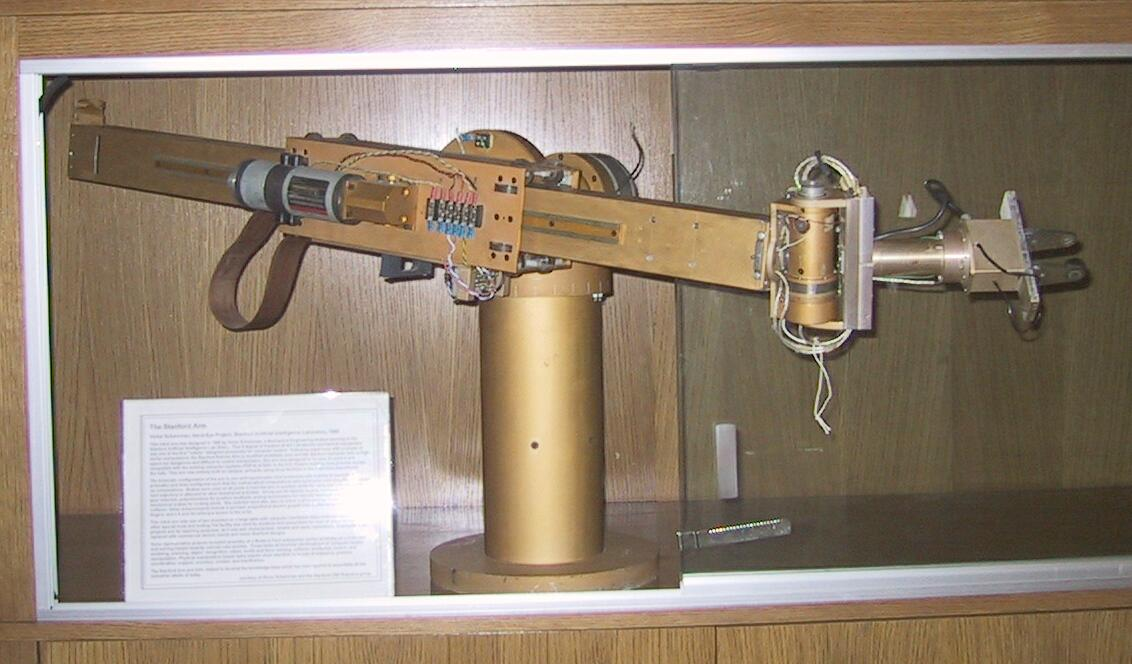
\includegraphics[width=0.50\linewidth ,height=0.4\columnwidth]{figures/StanfordArm.jpg} \,\,
 		&
 		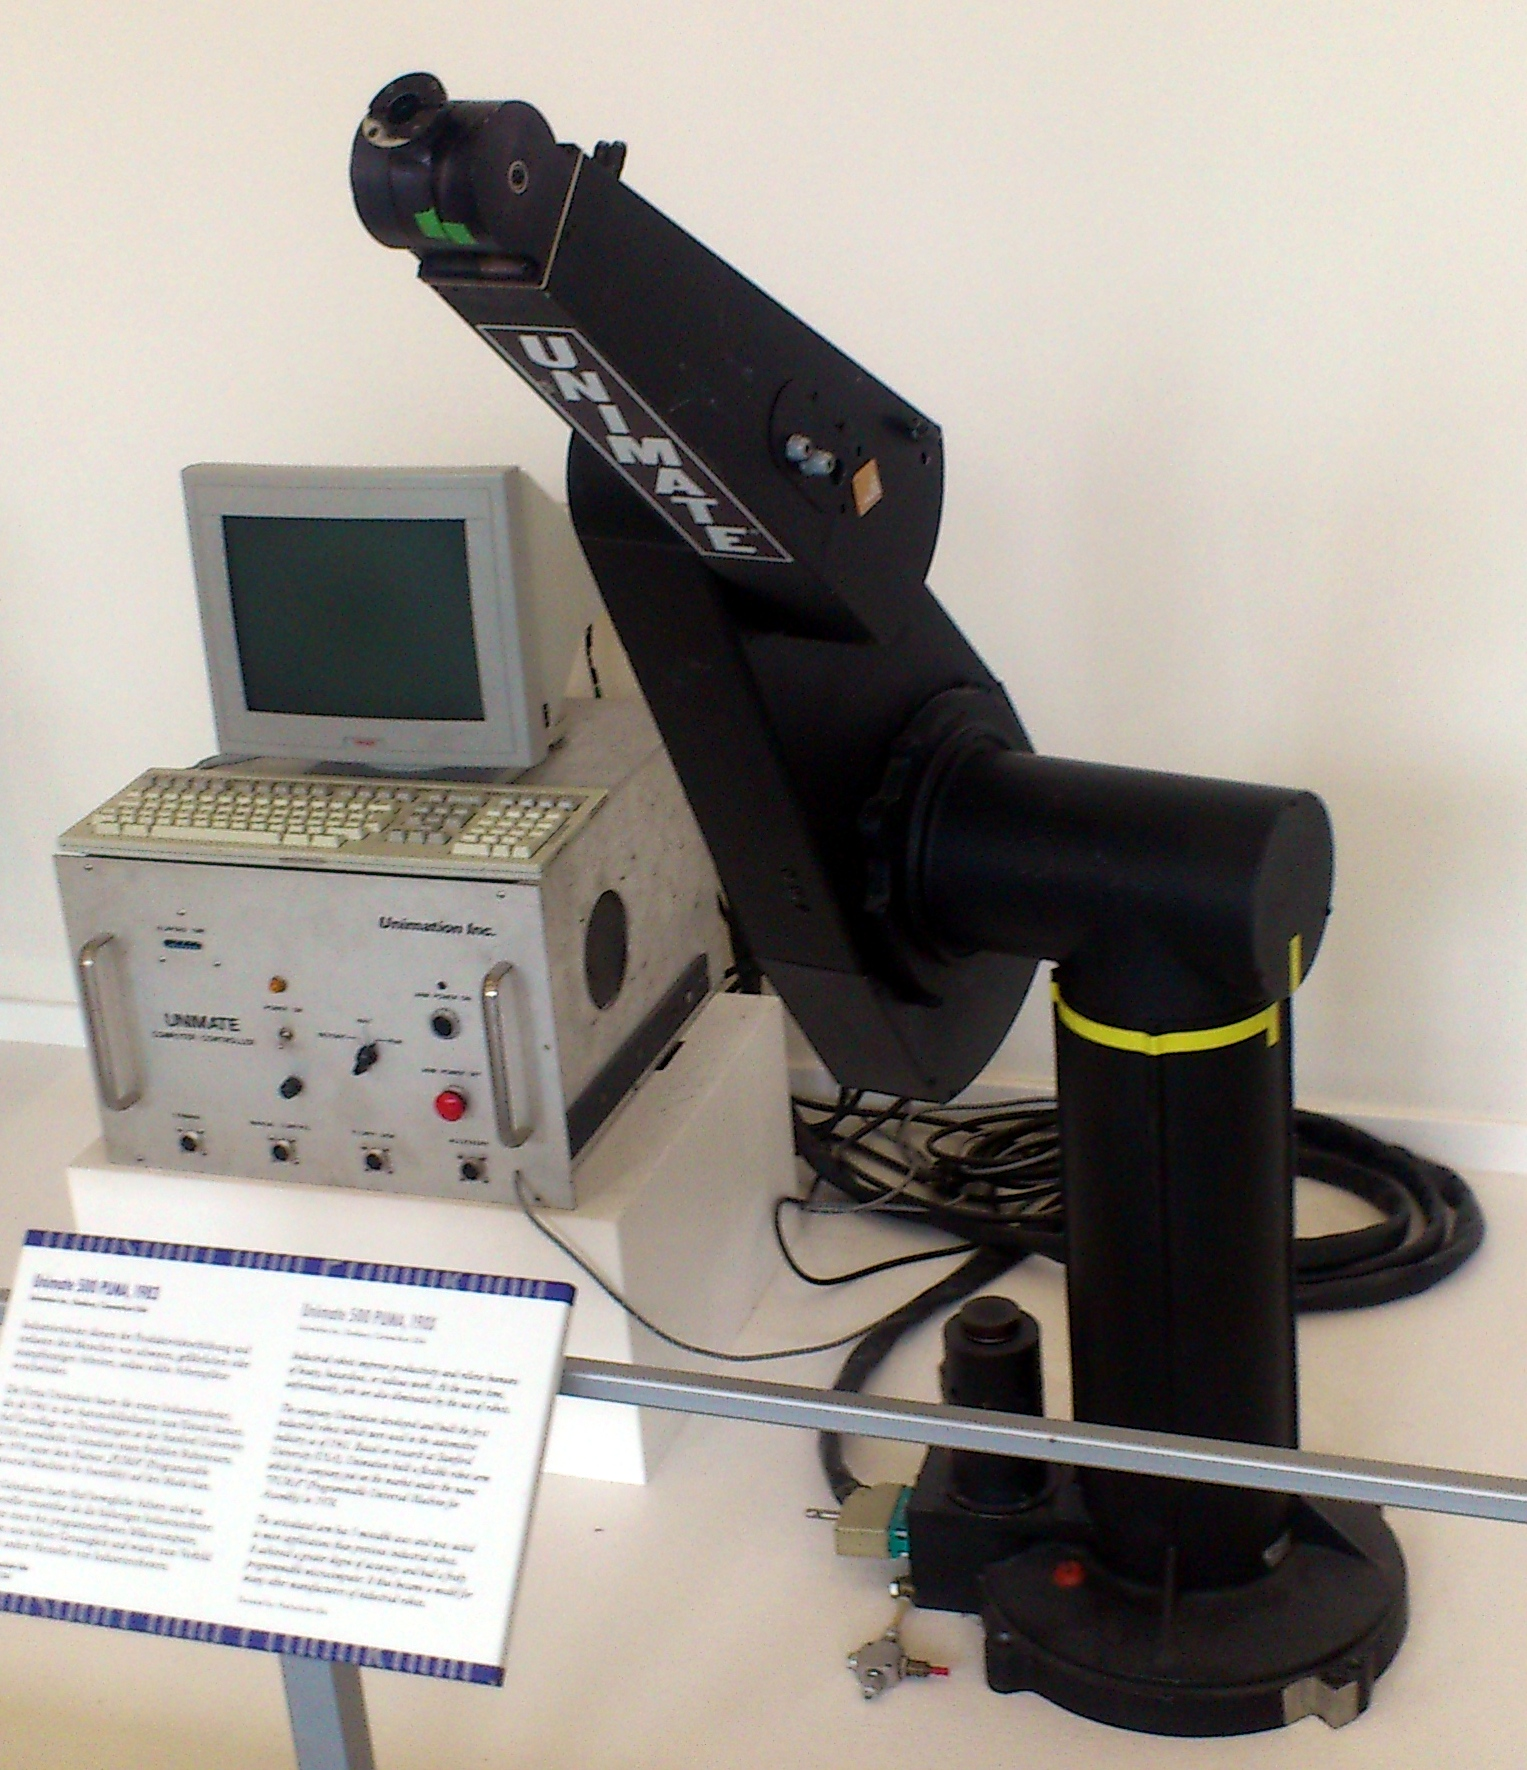
\includegraphics[width=0.48\columnwidth,height=0.4\columnwidth]{figures/PUMA.jpg}
 	\end{tabular}
 	\caption{Early serial kinematic chain robot manipulators. \textit{Left:} The Stanford Arm Serial Manipulator, 1969. \copyright Infolab, Stanford University. \textit{Right:}  The PUMA robot arm. Reprinted from Wikipedia.}
 	\label{fig:robot_arms}
 \end{figure}
 %
A kinematic chain is a form of a \textit{mechanism}. A ``\textit{mechanism can be interpreted as a means of transmitting, controlling, or constraining relative movement}"~\cite{HuntBook1977}. The term \textit{kinematics} is generally used to describe the motion of a rigid body in space. It also applies to the motion of a semi-rigid or a  completely soft robot in space.  The rigid, semi-rigid or completely soft kinematic systems that allow a body to exhibit motion under a/some controlled motion of its freedom in space with respect to a fixed base frame are what we describe in this module.
 %

\begin{figure}[tb!]
	\centering
	\begin{tabular}{@{}c@{}c@{}}
		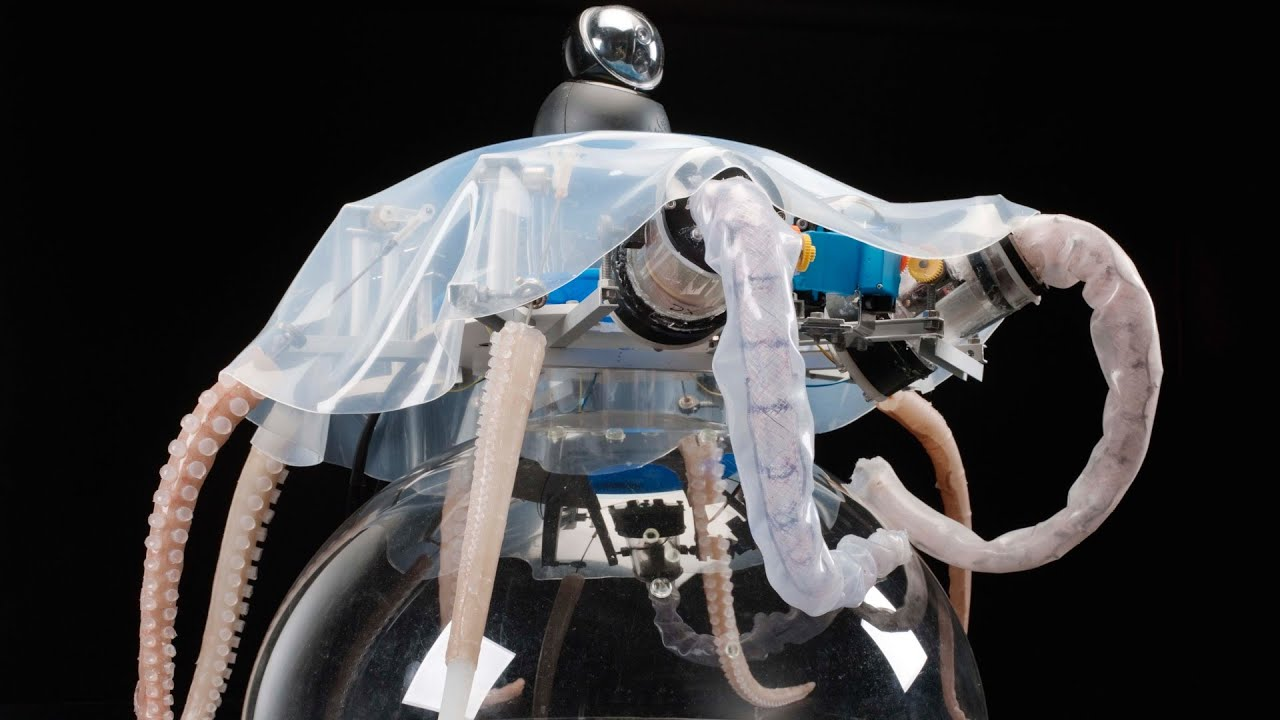
\includegraphics[width=0.50\linewidth ,height=0.4\columnwidth]{figures/octopus.jpg} \,\,
		&
		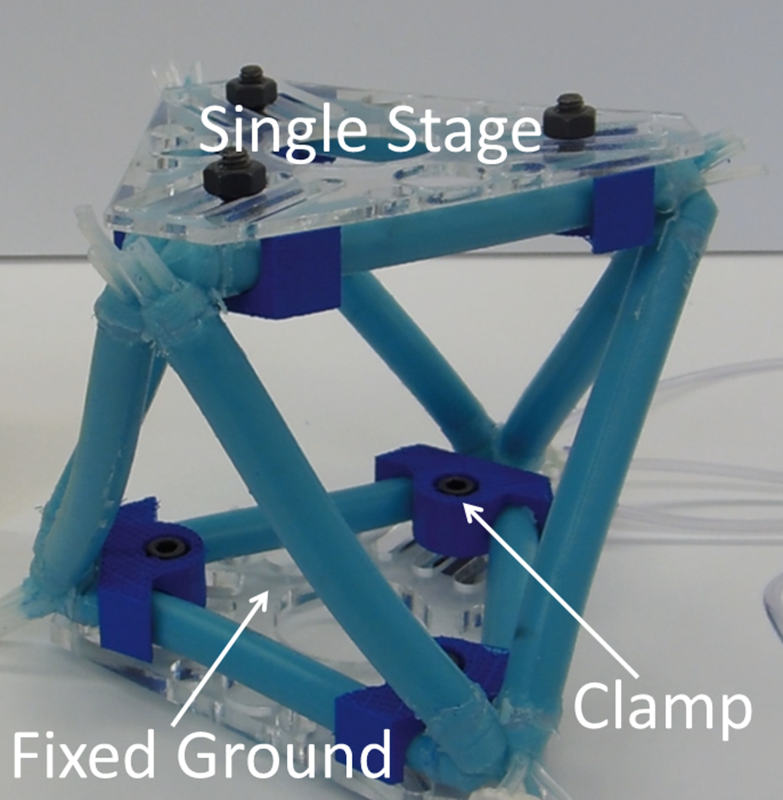
\includegraphics[width=0.48\columnwidth,height=0.4\columnwidth]{figures/soft_parallel.png}
	\end{tabular}
	\caption{Soft Robot Manipulators \textit{Left:} An octopus inspired soft robot. Robots classified under muscular hydrostats. \copyright Cecilia Laschi. \textit{Right:} A soft parallel robot manipulator ~\cite{hopkins2015synthesis}.}
	\label{fig:soft_robots}
\end{figure}

 \section{Robots Components}
 
The joints of a robot can be \textit{revolute} or \textit{prismatic}. Revolute joints allow rotation about a fixed axis between two or more links while prismatic joints allow a linear motion about an \textit{axis} -- which is between two links. Symbolically, the revolute joint is denoted by $R$ while the prismatic joint is denoted by $P$. By this logic, it follows that a robot made up of three links that are connected by a prismatic joint would be characterized as a $PPP$ arm, while a three link arm whose links are all connected by three rotary joints would be denoted as an $RRR$ arm. 
 
 A mathematical way to abstract the interconnection between the links of a robot arm is to denote the axis of rotation or the axis of translation by $z_i$ for the joint that connects link $i$ to link $i+1$. When we characterize the robot's motion, it often helps to work in a so-called \textit{generalized coordinate}. Now consider a rigid body such as a link of a robot arm for example. This link contains myriads of particles, with each particle having its own position and orientation in the world. How can we describe the motion of this rod given its infinitely many particulate matter? For rigid bodies, classical mechanics comes to the rescue. As such, for a revolute joint of a rigid robot manipulator for example, the generalized coordinate is often the \textit{joint angle} $\theta$, while for a prismatic joint it is the link length $d$ -- representing the relative displacement between adjacent links. When the body we speak of is a continuum, the motion of each particle within a link needs to be accounted for. In such scenarios, researchers often work with a so-called a \href{http://web.mit.edu/hyperbook/Patrikalakis-Maekawa-Cho/node25.html}{Frenet-Serret} frame that models  a curve on the soft robot's surface -- with or without torsion. This simplifies the dynamics and kinematics of the system and the specification of these generalized coordinates uniquely determines the position of all the particles (in a material sense for a rigid system) that make up the robot. For more examples on parameterizing soft robots, please look through some of the following references: \cite{Ogunmolu15CASE}, \cite{Hannan2000} \cite{Ogunmolu16CASE}, \cite{Renda2018ICRA}, \cite{ShepherdMultigait}, \cite{Hannan2003}, \cite{Ogunmolu17IROS}, \cite{Laschi15NeuNet}, \cite{Ogunmolu19RALI}, \cite{Renda2014Cosserat}, \cite{Ogunmolu19RALII}, \cite{OgunmoluThesis}.
% 
 
 \section{Robot Spaces, Geometries, and Classifications}
 
 The location of a robot in the world is described by its \textit{configuration}. This configuration specifies the positions of all points of the robot. While the coordinates of these points may be multiple over a continuous range of real numbers, the smallest number of independent variables of these real-valued coordinates needed to represent the robot configuration are the \textit{degrees of freedom} of the system.  In general, a \textit{free rigid body} has six degrees of freedom. The motion of the robot could be about a translation or rotary axis. The $n$-dimensional space that contains all the possible configurations of the robot is the \textit{configuration space} (or \textit{C-space}) of the robot. The configuration of the robot is expressed by a point in its C-space. 
 
 A manipulator with more than 6-\dof is said to be \textit{kinematically redundant}. %In general, the total number of the degrees of freedom of a \textit{rigid body} in space cannot exceed 6-\dof~\cite{Merlet2015}. 
 The set of variables that together with a description of the manipulator's dynamics and future inputs that determines the future transient response of the manipulator is the \textit{state} of the robot, while the set of all possible states is referred to as the \textit{state space}. For a rigid robot manipulator for example, the material and referential description alone is sufficient to describe the dynamics, which are Newtonian in nature. For such systems, the state may be specified by the joint variables $\{q, \dot{q}\}$ signifying the joint angles and joint velocities. For continuum systems, such representations are often inadequate. A popular method is to introduce a Frenet-Serret (you can read more about F-S frames in the link included earlier) frame on the body of the soft robot (SoRo) and characterize the state space based on the three parameters \ie $\{\mathcal{K}, l, \alpha\}$ that characterize the kinematic motion of the body viz., curvature of an arc projected on the SoRo's body, $\mathcal{K}$, the arc's length, $l$, and the angle subtended by a tangent along that arc, $\alpha$.
 
 \section{Characterization of Kinematic Geometry}
 %
 As mentioned earlier, disassociated from the dynamics (\ie forces, torques and such) of a body, that which deals with the displacements, or movements of a body relative to another within a mechanism is termed the \textit{kinematics}. The displacement could be linear, angular -- and in combination with the derivatives with respect to time of such displacements viz., velocities, accelerations, and hyper-accelerations all are part of the kinematics of a body. The other branch of \textit{dynamics}, called \textit{kinetics}, determines the forces, torques, energy, momenta, inertia, equilibrium and dynamic stability of the system and that is treated in a separate module in this course.
 
 \subsection{Kinematic Geometries}
 %
 Kinematic geometry deals only with the \textit{displacements} of a system in the first and simplest segment of kinematics.  In general, the use of time as a variable is shunned upon since the displacements we intend to carry out may be performed as fast as user wishes in their implementation (to be seen in  \autoref{chap:statics}.  For the rest of this subsection, by kinematics, we shall mean the displacement of rigid bodies or ``the solid geometry of relatively moving bodies". 
 
 The majority of robot arms (at least today) have their actuators (or joints) connected in series along an \textit{anthropomorphic} arm, with each joint being either at or associated with a single \dof in the robot arm. 
 %
\begin{figure}[tb!]
	\centering
	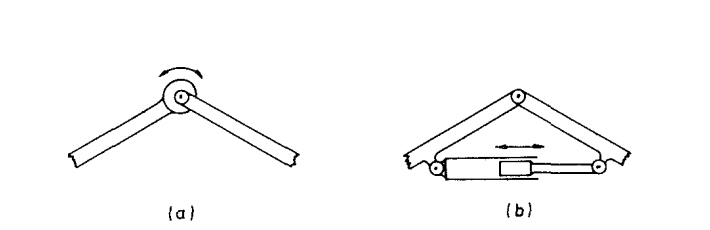
\includegraphics[width=\columnwidth]{figures/arms_hunt.png}
	\caption{Schematic description of in-series-actuated robot arms: (a) rotary joint actuated ``about" the hinge (b) prismatic joint actuated ``across" a hinge. Reprinted from \cite{Hunt1983}.}
	\label{fig:arms_schematic}
\end{figure}
%
\autoref{fig:arms_schematic} describes the two major ways rigid links are actuated today. From a geometric point of view, both types of actuation in \autoref{fig:arms_schematic} serve the same purpose, which is to control the rotation of the joint. However, when we are interested in controlling ``pure translation" such as sliding between links, non-pivoted linear actuators are used on their own. 


\subsection{Open Kinematic Chains}

When the links are serially connected to one another and there is no link that connects the base link to the tool frame, the robot is said to be in-series actuated. Series-jointed links have a major disadvantage, namely that they accumulate errors from shoulder out to end-effector and they suffer from a lack of rigidity. In order to eliminate their inherent load-dependent error, manufacturers typically stiffen them. However, this stiffening process increases the mass of the arm such that greater demand is placed on the actuation system. Some manufacturers employ  a compensated actuation or sophisticated control techniques in order to  overcome the load-dependent errors. 
%
\begin{figure}[t!]
	\centering
	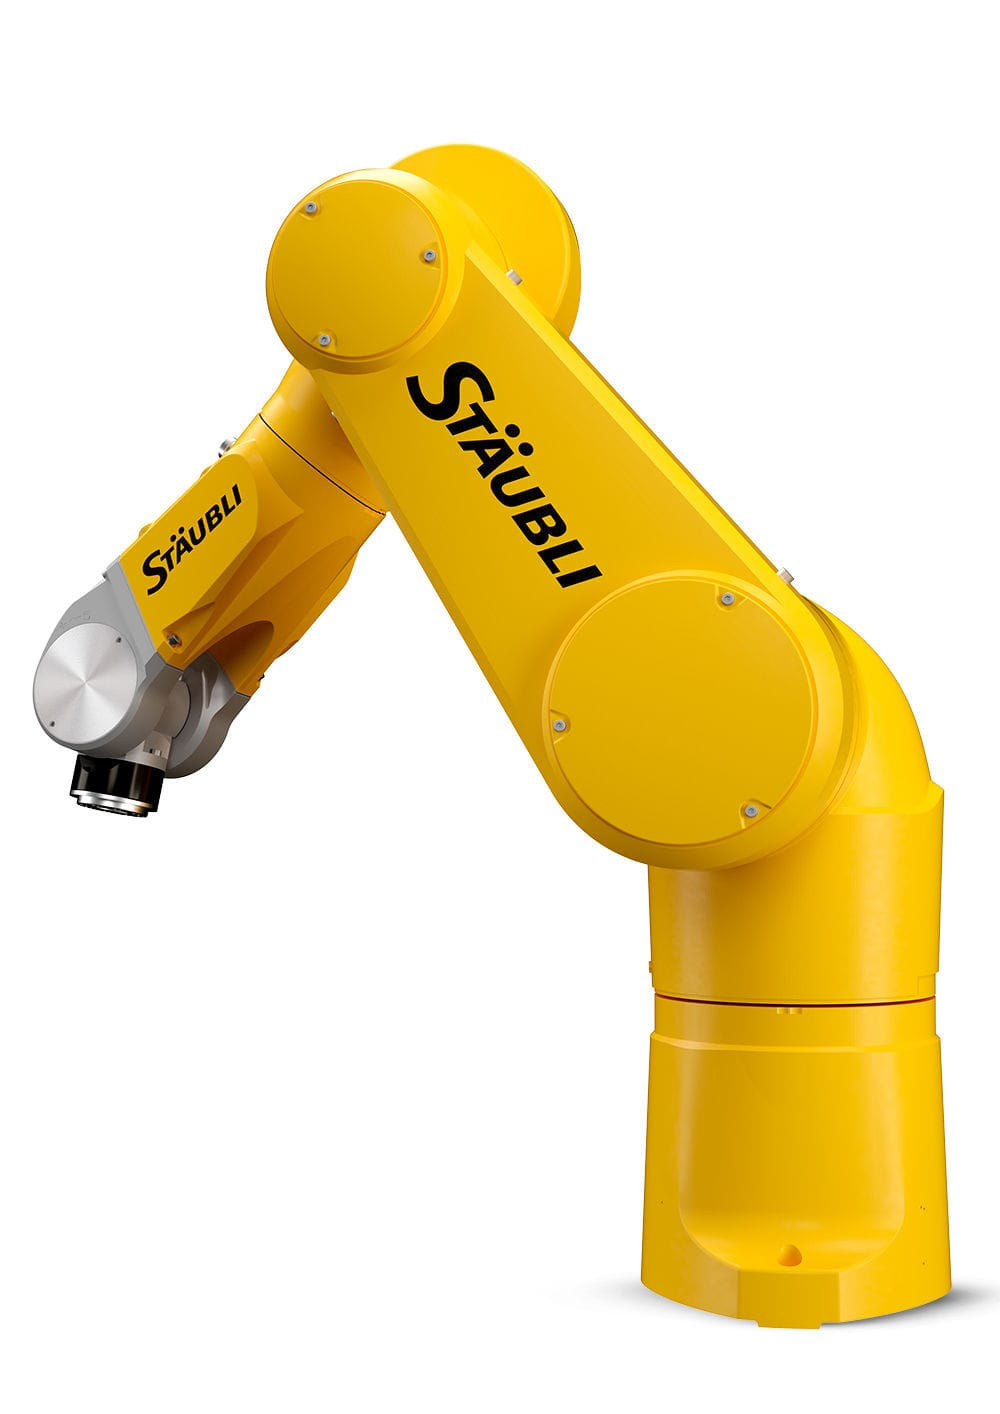
\includegraphics[scale=.1, width=.4\columnwidth]{figures/Staubli.jpg}
	\caption{The Staubli 6-DOF Arm is an example of a Spherical Manipulator. Reprinted from DirectIndustry's Webpage.}
	\label{fig:staubli}
\end{figure}

Examples of in-series actuated mechanisms is the \textit{spherical robot} (see \autoref{fig:scara_bot}), where a succession of the robot segments are linked to the predecessors by revolute joints. By actuating each of the $n$ joints we can control the $n$ degrees of freedom of the end-effector. 
%
\begin{figure}[b!]
	\centering
	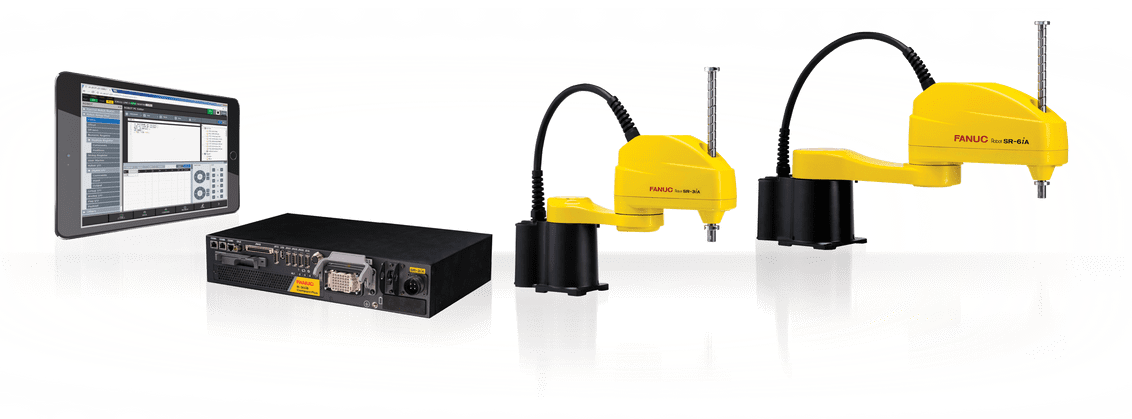
\includegraphics[width=\columnwidth]{figures/Scara.png}
	\caption{The SCARA Arm. \copyright Fanuc America.}
	\label{fig:scara_bot}
\end{figure}
%
The SCARA robot, shown in \autoref{fig:scara_bot} is an example that allows the control of the end-effector based on the geometry of the previously connected links. 

It is ideally desirable to keep the load-to-mass ratio of a robot as minimum as possible whilst preserving positioning accuracy. This is so as to preserve two important properties of the robot: repeatability (\ie the maximum distance between two positions of the end-effector reached for the same desired pose from different starting positions),  and absolute accuracy (\ie distance between the desired and actual position of the end-effector) respectively. Positioning accuracy is a function of the deformation of flexure -- typically not accounted for by the robot's internal sensors -- and the absolute accuracy. The absolute accuracy is a function of the sensors at the manipulator joints, the clearance for the drive, flexure of links, and geometric accuracy of link orientations inter alia. When geometric constraints are violated (take a small error in the perpendicularity between successive links of a spherical arm, for example), large errors are bound to occur in the vertical motions so that such errors must be accounted for during manufacture. The conventional approach to overcoming this currently is for manufacturers to stiffen the robot's links. However, stiffening the links is tantamount to overall heavier mass, which in turn means the manipulator experiences higher inertia, centrifugal and Coriolis forces -- these complicate motion planning for complex trajectories.  

As we close this part of the module, bear in mind that open kinematic chains are governed by inertia and centrifugal forces -- forces that exist on different scales. For example, inertia forces are a function of the square of the link lengths while frictional forces are not affected by the such dimensions. As such, serial robots cannot be scaled down to a micro level as inertia forces would be reduced while frictional forces would remain unchanged. It is not surprising that these attributes listed make serial manipulators exhibit poor positioning accuracy. 

\subsection{Closed-loop Kinematic Chains}
 
 When the number of links connected to a joint (the \textit{connection degree}) is more than 2, we have a closed-loop kinematic chain. Closed-loop kinematic chains resolve the accuracy problems of open-loop chains by mechanically distributing the load on the links: they link the end-effector to the ground by a set of links that support only a fraction of the load. While theoretical works that envisioned parallel mechanisms have been in existence since 1645~\cite{Merlet2015}, the Stewart~\cite{Stewart1965} and Gough~\cite{Gough1957} platforms are the original designs of closed-loop chains on record. 
 %
 \begin{figure}[tbph!]
 	\centering
 	\begin{tabular}{@{}c@{}c@{}}
 		\includegraphics[width=0.50\linewidth ,height=0.4\columnwidth]{../../Papers/PhDThesis/figures/GoughPlatform.png} \,\,
 		&
 		\includegraphics[width=0.48\columnwidth,height=0.4\columnwidth]{../../Papers/PhDThesis/figures/GoughPlatformNow.jpg}
 	\end{tabular}
 	\caption{Stewart-Gough Platforms \textit{Left:} The 1954 Octahedral hexapod of the original Gough platform. \textit{Right:} The retired platform from Dunlop tires in 2000. Picture courtesy of Parallemic.org.}
 	\label{fig:stewart_gough}
 \end{figure}
%
The mechanical arrangement of the links of the platform help with the load-to-mass ratio: the manipulator mass is reduced, and the disturbing effects of the Coriolis forces decreases. Albeit, these manipulators typically have a smaller workspace.
Formally, we define a \textit{generalized parallel manipulator} as a closed-loop kinematic chain mechanism whose end-effector is linked to the base by many independent kinematic chains~\cite{Merlet2015}.
 
 \section{Freedom and Structure in Mechanisms}
 
 Early on, we briefly defined what constitutes the degrees of freedom of a rigid body. We will now systematically analyze how to determine the mobility of a mechanism given its \textit{kinematic pairs}, linkages and freedoms.
 
 \subsection{Freedom, Connectivity and Mobility}
 
 For every \textit{kinematic pair}\footnote{Bonus homework: Research what is a kinematic pair and produce a one-page written report.}, there exists a characteristic number of the degrees of freedom that characterize its mobility.  If a kinematic pair has elements that touch at a single point, we would have five degrees of freedoms -- two of which would be translatory and three rotary. A kinematic pair whose elements always touch along a line or a curve has four or fewer degrees of freedom, or for short, freedom (see \autoref{fig:kinematic pair}).
%
\begin{figure}[tb!]
	\centering
	\emptybox{4cm}
	%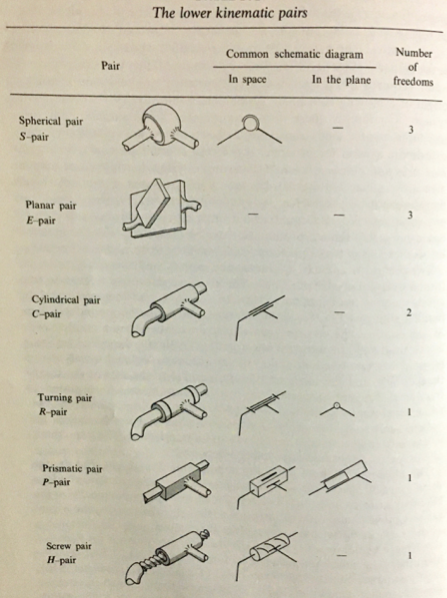
\includegraphics[width=\columnwidth, height=.5\columnwidth]{figures/kinematic_pair.png}
	\caption{Insert Kinematic Pair Table here}
	\label{fig:kinematic pair}
\end{figure}

However, in mechanisms, we are more concerned about the relative motion between objects in the mechanisms that do not directly touch one the other. In such systems, what we do is consider the freedom that is contributed by each of the several kinematic pairs that connect them. For the popular four bar linkage, for example (see ~\cite{MurrayBook}), the four $R$-pairs on the two connectivity-links 2 and 4 complete a \textit{coupling} or \textit{connection} between 1 and 3. This is said to have a connectivity of $1$, typically written as $\mathscr{C}_{13}=1= \mathscr{C}_{31}$. Note that here, all connectivities are the same , and $\mathscr{C}_{ij} = 1$, for $i \neq j$ and $i,j=1,2,3,4$. Now, suppose that the $R$ pairs are replaced by spherical, or for short, $S$ pairs, then we have an additional so-called \textit{spin-freedom} about the $SS$ axis (see figure \autoref{fig:four_bar})
%
\begin{figure}[tb!]
	\centering
	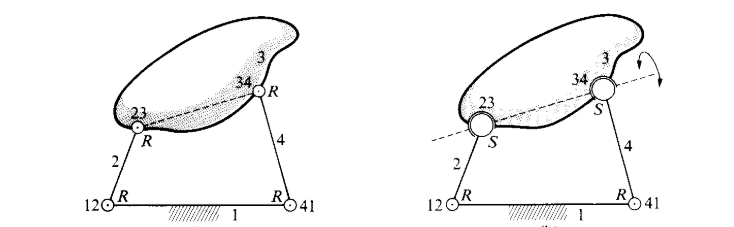
\includegraphics[width=\columnwidth]{figures/four-bar-linkage.png}
	\caption{The planar $RRR$ linkage, (\textit{left}) is modified in (\textit{right}) to allow spatial spin-movement of the coupler 3; the connectivity $\mathscr{C}_{13}=2$). Reprinted from ~\cite{HuntBook1977}.}
	\label{fig:four_bar}
\end{figure}
%
so that $\mathscr{C}_{13}=2$. In any case, $\mathscr{C}_{12}=\mathscr{C}_{13}=\mathscr{C}_{43} = 2$.

Related to the concept of connectivity and more popular in literature is the concept of \textit{relative mobility} or simply \textit{mobility}.  The mobility, $\mathfrak{M}$, is usually referred to as the number of \textit{degrees of freedom} of a mechanism. To specify the independent variables needed to determine all the relative locations of the complete members of a mechanism with respect to one another, we typically use the \textit{mobility criterion}. As such, we would have the kinematic chain of the left inset of \autoref{fig:four_bar} having $\mathfrak{M}=1$ since only an angle between the elements of any of the four kinematic pairs is required so as to prevent all relative movement. However, for the $RSSR$ mechanism on the right of \autoref{fig:four_bar}, the mobility would be $\mathfrak{M}=2$ since member $3$ has a spin-freedom.

\begin{tcolorbox}[title=Determining Degrees of Freedom]
	\textit{Screw Coordinates} are better suited -- from a kinematic standpoint, at any rate -- to determine the general and impartial location of a rigid body.
\end{tcolorbox}

\subsection{Constraints and Freedoms}
%
In rigid body kinematics, it is a given that the freedoms of a \textit{free rigid body} is $6$. But how is this determined? Suppose we have six homogeneous \textit{screw coordinates} (to be introduced shortly) $x_1, x_2, \ldots, x_6$, we find that the body is fixed when values are attached to all six of them. However, the physical constraining system to which the body is subjected is not likely to have for every constraint exactly one corresponding independent screw coordinate For every constraint in the system, there is an influence on each of the six coordinates. For every independent constraint, a freedom of the body is suppressed so that the six independent constraint-equations $f_i(x_1, x_2, \ldots, x_6)=0, \, i = 1, 2, \ldots, 6$ must all be simultaneously satisfied. We define the \textit{condition} as the constraint equation that describes a particular constraint algebraically. As the constraints are progressively relaxed, the corresponding constraint-equations are struck out one after another, so that the body acquires one, two, $\ldots$, degrees of freedom, until the body is completely free with no constraints or equations and we end up with six freedoms. Suppose the number of freedoms is $f$ and the number of \textit{unfreedoms} or constraints is $u$, it turns out that 
%
\begin{equation}
	u + f = 6.
	\label{eq:unfreedom}
\end{equation}

\subsection{The Mobility Criterion}

For $g$ working joints between a total of $n$ bodies, the number of relative degrees of freedom can be identified with the relative mobility of the system of bodies, described as 
%
\begin{align}
	\mathfrak{M} = 6(n-1) - \sum_{i=1}^{g} u_i
	\label{eq:mob_bodies}
\end{align}
%
where the summation term aggregates over all individual unfreedoms. Plugging \eqref{eq:unfreedom} into  \eqref{eq:mob_bodies}, we have 
%
\begin{align}
\mathfrak{M} = 6(n-1) -\sum_{i=1}^g 6 + \sum_{i=1}^{g} f_i
\end{align}
%
or 
%
\begin{align}
\mathfrak{M} = 6(n - g - 1) + \sum_{i=1}^{g} f_i.
\label{eq:mob_cond_gen}
\end{align}

Equation \eqref{eq:mob_cond_gen} is termed the general mobility criterion. It is attributed to Gr\"ubler (1908 and 1917), and independently to Kutzbatch (1929). In this module, we will generally call it the Gr\"ubler-Kutzbach's mobility criterion. When there are independent kinematic chains within the body of concern, it is sometimes more convenient to write \eqref{eq:mob_cond_gen} as 
%
\begin{align}
	\mathfrak{M} = \sum_{i=1}^g f_i - 6c
	\label{eq:mob_loop}
\end{align}
%
with $c$ being the number of independent chains. 

There are exceptions to the Gr\"ubler-Kutzbach's mobility criterion such as when we have planar or spherical mechanisms. Take the four-bar linkage for example. There are four freedoms to the kinematic pairs, yet patently it has a mobility of $\mathfrak{M}=1$, and not $\mathfrak{M}=-2$ as \eqref{eq:mob_loop} would have us so determine it.  This is because for planar and spherical mechanisms, the number of freedoms is not six as in \textit{general} space, but three. Therefore, we write out the special version of \eqref{eq:mob_cond_gen} as 
%
\begin{align}
\mathfrak{M} = 3(n - g - 1) + \sum_{i=1}^{g} f_i.
\label{eq:mob_cond_planar}
\end{align}
%
This special nature of \eqref{eq:mob_cond_planar} arises because the joints' freedoms are not independent in planar motion, because the axes of the turning pairs are all directed parallel to one another, any prismatic pair being perpendicular to them. For spherical motions, the turning axes co-intersect at a single point.

\begin{homework}
	%\newline
	\begin{itemize}
		\item Read up on the common kinematic arrangements in Section 1.3 of Spong and Vidyasagar and produce a 2-page single-spaced summary report. Your report must not contain diagrams but feel free to do as much analysis of the configurations of the various kinematic arrangments that are mentioned.
		%
		\item Using the mobility condition, determine and explain why the SCARA robot of \autoref{fig:scara_bot} has the number degrees of freedom that you find.
		%
		\item For the mobile manipulator we are using in this course, analyze the connectivities and freedoms of the kinematic pairs in the mechanism. In addition, determine the freedom of the overall mechanism and write out the mobility criterion.
		%
		\item With the \textit{{Gr\"ubler-Kutzbach's} mobility condition} that we have learned, analyze the mobility criteria of the mechanism of \autoref{fig:para_mech}. Hint: This mechanism is made up of two chains: chains $A_3\, B_3\, B_1\, A_1$ and $A_2\, B_2\, B_4\, A_4$, and there is a fixed distance between the $U$-joints, $A_2\, A_3$ as well as $A_1, A_4$.
		%
	\end{itemize}
\end{homework}


\begin{figure}[tb!]
	\centering
	\begin{tabular}{@{}c@{}c@{}}
	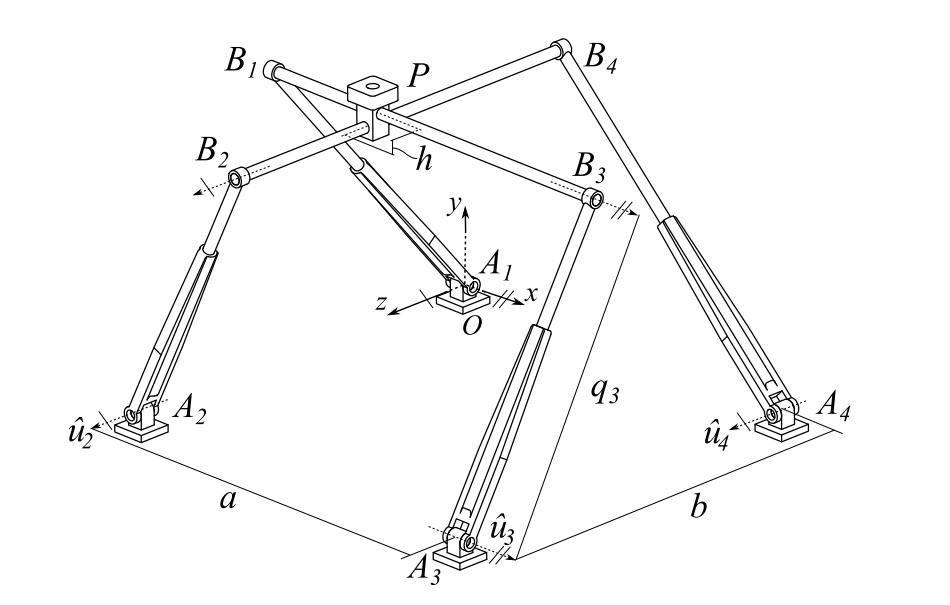
\includegraphics[width=0.50\linewidth ,height=0.4\columnwidth]{figures/parallel_translational.png} \,\,
	&
	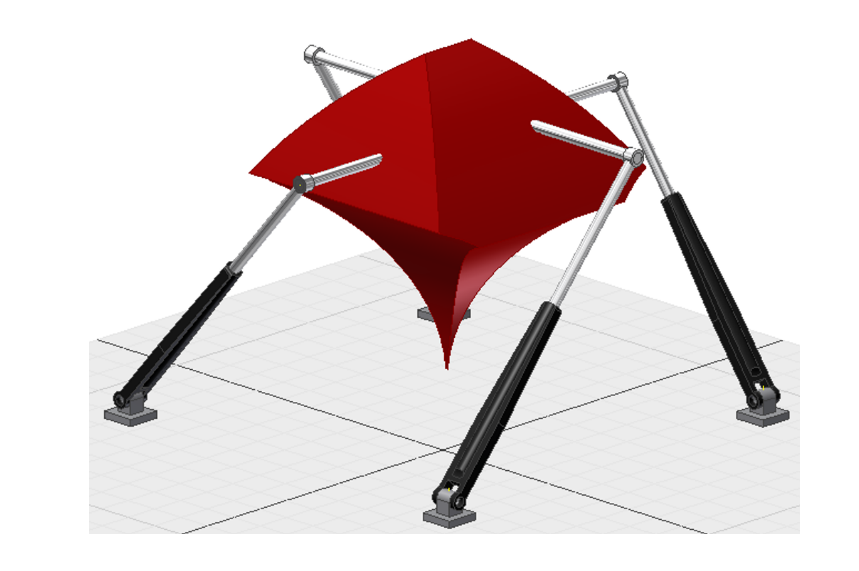
\includegraphics[width=0.48\columnwidth,height=0.4\columnwidth]{figures/parallel_translational_workspace.png}
	\end{tabular}
	\caption{\textit{Left}: A Parallel Planar Robot Mechanism. \textit{Right:} Workspace of the mechanism.}
	\label{fig:para_mech}
\end{figure}
\chapter{Motion of Rigid Bodies}
\label{chap:rbm}

In this chapter, we shall lay the foundations for analyzing the kinematics of a rigid or soft body in general space. Our goal is to present a geometric view of the translational and rotational rigid body motions. We take the classical screw theory approach owing to its simplicity in analyzing the geometry of kinematic motions compared against the common Denavit-Hartenberg (DH) conventions. We leave the treatment of the DH convention as an exercise for the reader. While the materials presented here may appear abstract, the applications are practical and useful. Therefore in reading the materials presented forthwith, it is recommended to the reader to ask what is it to the kinematic geometry of mechanisms that we have labored upon in \autoref{chap:intro}. The recommended texts for this chapter are 

\begin{itemize}
	\item Murray, R. M., Li, Z., \& Sastry, S. S. (1994). A Mathematical Introduction to
Robotic Manipulation . Book (Vol. 29), Chapter 2
	%
	\item A treatise on the theory of screws, Sir R.S. Ball, Chapter 1
	%
	\item Screw theory for robotics, Jose M. Pardos-Gotors, IROS2018 tutorial; (Email the instructor for a copy).
	%
\end{itemize}


\section{Screws}

Simply put, \textit{a screw is a line (called an axis) by which a definite linear magnitude (termed the pitch, $p$) is associated}.
%What follows is based on the thesis of Kenneth Salisbury~\cite{Salisbury}. 
%A \textit{screw} is defined collectively by a straight line in space called an \textit{axis} which has an associated \textit{pitch}, $p$, and a magnitude, $\ell$.  
A screw may be defined by a 6-vector of \textit{screw coordinates}, $\underline{s}=(S_1, S_2, S_3,S_4, S_5, S_6)$ which has the following interpretations in terms of the Pl\"ucker line coordinates of the axis
%
\begin{subequations}
	\begin{align}
	L &= S_1, \quad M = S_2, \quad N=S_3,   \label{eq:plucker_line} \\ 
	%
	P &= S_4 - pS_1, \quad Q = S_4 - pS_2, \quad R = S_6 - pS_3
	\label{eq:plucker_mom}
	\end{align}
\end{subequations}
%
where $L, M, N$ are proportional to the direction cosines of the line forming the axis while $P, Q, R$ are proportional to the moment of the line about the origin of the reference frame. If we scale the Plucker coordinates by $(L^2 + M^2 + N^2)^{1/2}$, the first three would represent the direction cosines of the line while the last three would represent the moments. We have the moment of the line as the cross product of a vector from the reference frame's origin to any point on the line with the unit vector in the line direction. Thus, we have the pitch of the screw defined as 
%
\begin{align}
	p = \dfrac{S_1\,S_4+S_2S_5+S_3S_6}{S_1^2+S_2^2+S_3^2}
\end{align}
%
whose magnitude is 
%
\begin{align}
	\|\ell \|^2 = S_1^2+S_2^2+S_3^2
\end{align}
%
for a finite pitch, otherwise, it is
%
\begin{align}
\|\ell \|^2 = S_4^2+S_5^2+S_6^2
\end{align}
%
for an infinite pitch. Note that  for infinitesimal screws, scalar multiplication and vector addition are valid so that two screws, $\underline{s}_1$ and $\underline{s}_2$ are considered linearly dependent if there exists non-zero scalars, $c_1$ and $c_2$ \ie $c_1\underline{s}_1+c_2\underline{s}_2=0$.


\subsection{Motion screws: Twist's Pitch, Axis, and Magnitude}
%
The unique line about which a body in space rotates or translates for an infinitesimal motion or velocity of the body is called the \textit{twist axis}. Formally, we say \textit{a body receives a twist about a screw when it is uniformly rotated about the screw, while it is translated uniformly parallel to the screw, through a distance equal to the product of the pitch and the circular measure of the angle of rotation}~\cite{Ball}. 

Similar to the screw, the \textit{twist} is characterized by a six-vector of coordinates, $\underline{t}=(T_1, T_2, T_3, T_4, T_5, T_6)$ so that the components of the angular velocity of the body are denoted by $\underline{w}=(T_1, T_2, T_3)$ while the components of the linear velocity of a fixed point in the body lying at the origin of the coordinate system is $\underline{v}\equiv(T_4, T_5, T_6)$. 

An important thing to note is that the a twist is characterized by the attributes \textit{pitch, magnitude and an axis}.  Hence, we have the Pl\"ucker coordinates of the \textit{twist axis} given as
%
\begin{definition}[Twist Axis]
	
	\begin{subequations}
		\begin{align}
		L &= T_1,\quad M=T_2, \quad N=T_3 \\
		%
		P &= T_4 - pT_1, \quad Q=T_5-pT_2, \quad R = T_6 - pT_3.
		\end{align}
	\end{subequations}
\end{definition}
%
\begin{definition}[Pitch of a Twist]
	The pitch of the twist, $\twistcoord = \left(\begin{array}{cc}
	\omega & v
	\end{array}\right)^T$ is 
	%
	\begin{align}
	p = \ifelse{\dfrac{T_1T_4+T_2T_5+T_3T_6}{T_1^2+T_2^2+T_3^2} = \dfrac{\underline{w}^T\cdot \underline
			{v}}{\underline{w}\cdot \underline{w} }}{\underline{\omega} \neq 0}{\infty} .
	\label{eq:twist_pitch}
	\end{align}
\end{definition}
%
\begin{definition}[Magnitude of a Twist]
	The magnitude of the twist, $\twistcoord = \left(\begin{array}{cc}
	\omega & v
	\end{array}\right)^T$ is 
	%
	\begin{align}
	\|\twistcoord \| = \ifelse{\|\underline{\omega}\|}{\underline{\omega}\neq 0}{\|\underline{v}\|} .
	\label{eq:twist_mag}
	\end{align}
\end{definition}


In screw theory, it is typical to concern ourselves only with the small displacements of a system's motion. Whenever a body admits an indefinitely small movement of a continuous nature, it is capable of executing that kind of movement denoted by a twist about a screw. When the body receives twists in several succession, the position that is finally attained is called the \textit{resultant twist}.

\noindent 
\begin{homework}
	What is the geometric meaning of \eqref{eq:twist_pitch} on a twist axis to you. Define \textit{pure rotation} and a \textit{pure translation} in terms of \eqref{eq:twist_pitch}\footnote{Figure out how they correspond to zero pitch and infinite pitch twists.}. 
\end{homework} 

\subsection{Dynamics Screws: Twist's Pitch, Axis, and Magnitude}
%
For a set of forces and moments applied to a rigid body, there is a \textit{wrench axis}, a unique line, which has associated with it a pitch, $p$, and a magnitude. We may consider the set of forces and moments that act on the body to be a single force along  the wrench axis and a a moment about exerted about the axis. This force-moment pair is termed a \textit{wrench}, and it is characterized by the 6-vector $\underline{w} = (W_1, W_2, W_3, W_4, W_5, W_6)$. We consider the first three components of $\underline{w}$ to be the net force components, $\underline{f}$, exerted on the body and $\underline{m}=\{W_4, W_5, W_6\}$ to be the components of the net moment resolved at the origin of the reference frame. We define the Pl\"ucker coordinates of the \textit{wrench axis} as 
%
\begin{subequations}
	\begin{align}
	L &= W_1, \quad M=W_2, \quad N = W_3 \\
	P&= W_4-pW_1, \quad Q = W_5 - pW_2, \quad R=W_6 - pW_3
	\end{align}
\end{subequations}
%
with pitch defined as
%
\begin{align}
	p = \dfrac{W_1 W_4 + W_2 W_5 + W_3 W_6}{W_1^2 + W_2^2+W_3^2} = \dfrac{\underline{f} \cdot \underline{m}}{\underline{f} \cdot \underline{f}}.
	\label{eq:wrench_pitch}
\end{align}
%
Equation \eqref{eq:wrench_pitch} signifies that the pitch of the wrench is the ratio of the magnitude of the applied moment about a point to the magnitude of the applied force along a wrench axis. A \textit{zero pitch wrench}  would therefore correspond to pure force while an infinite pitch wrench would be a pure moment. We define the magnitude of the wrench as $\|\underline{f}\| = \sqrt{W_1^2 + W_2^2 + W_3^2}$ when we have a finite pitch. If the pitch in infinite, the magnitude is $\|\underline{m}\| = \sqrt{W_4^2 + W_5^2 + W_6^2}$.

\noindent 
\begin{homework}
	A unit screw, twist or wrench is one where the magnitude of the screw, twist or wrench is $1$.  
	
	(1). What is the geometric meaning of a unit screw to you? %Often with twist and wrenches we wish to associate a magnitude other than 1 so that there are $\infty^6$ different twists and wrenches if we consider their magnitudes as well. With this interpretation we can think of a unit screw as defining only an axis and a pitch. Then we can think of a given magnitude as defining a twist (if its units are rotation/time) or a wrench (if its units are force) acting along the screw. In both cases the pitch is expressed in length units. These six-spaces of (infinitesial) twists or wrenches can be considered to be vector spaces in tha t they are closed under vector addition and scalar multiplication.
	(2) Consult the identified reference materials and explain what a reciprocal screw is in no more than five sentences.
\end{homework}


\subsection{Screw Motions}

A \textit{screw motion} is a rotation about the axis, $l$ by an amount $\alpha = \ell$ followed by a translation by an amount $h\alpha$ that is parallel to the axis $l$. A pure translation occurs when $h=\infty$ so that the screw motion is composed of a \textit{pure translation} along the axis of the screw by a distance $\ell$. 



\section{Rodrigues' Formula}
%
The matrix exponential
%
\begin{align}
	e^{\hat{\omega}t} = I + \hat{\omega}t + \dfrac{(\hat{\omega}t)^2}{2!} + \dfrac{(\hat{\omega}t)^3}{3!} + \cdots
\end{align}
%
is instrumental in defining the rotation about an axis, $\omega$: 
%
\begin{align}
	R(\omega, \theta) = e^{\hat{\omega} \theta}.
\end{align}
%
Thus, for a matrix $\hat{\omega}$ in the Lie algebra ${so}(3)$, a unit vector $\|\omega\| = 1$, and a real number $\theta \in \bb{R}$, we write the exponential of $\hat{\omega} \theta$ as
%
\begin{align}
e^{\hat{\omega}\theta} = I + \theta \hat{\omega} + \dfrac{\theta^2}{2!}\hat{\omega}^2 + \dfrac{\theta^3}{3!}\hat{\omega}^3 + \cdots
\end{align}

\noindent 
\begin{homework}
	Given a matrix $\hat{m} \in so(3)$, suppose that the following relation holds,
	%
	\begin{align}
	\hat{m}^2 = m m^T - \|m\|^2 \identity \\
	%
	\hat{m}^3 = - \|m\|^2 \hat{m}
	\end{align}
	%
	with the fact that higher powers of $\hat{m}$ can be recursively found. Therefore, utilizing this lemma with $m =\omega \theta$, $\|\omega\| = 1$, show that 
	%
	\begin{align}
	e^{\hat{\omega}\theta}  = \identity + \hat{\omega} \sin \theta + \hat{\omega}^2(1 - \cos \theta).
	\label{eq:rodrigues}
	\end{align}
\end{homework} 
%
Equation \eqref{eq:rodrigues} is \textit{Rodrigues' formula}.


\section{The Matrix Exponential, The Lie Group and Lie Algebra}
%
For any matrix 
%
\begin{align}
\homo = \begin{bmatrix}
\rot & \disp \\
0 & 1
\end{bmatrix} \in SE(3) \text{ such that } \rot \in SO(3), \disp \in \bb{R}^3, \text{ and } \rot\rot^T = \identity
\end{align}
%
there exists a matrix 
%
\begin{align}
N = \begin{bmatrix}
\skew & x \\
0 & o
\end{bmatrix} \text{ such that } \skew = -\skew^T
\end{align}
%
such that $\exp(N) = \homo$ since we can write
%
\begin{align}
\begin{bmatrix}
\rot & \disp \\
0 & 1
\end{bmatrix}  
%
&=  \begin{bmatrix}
\identity & \disp \\
0 & 1
\end{bmatrix}
%
\begin{bmatrix}
\rot & 0 \\
0 & 1
\end{bmatrix}  =  \begin{bmatrix}
\identity & \disp \\
0 & 1
\end{bmatrix} 
%
\exp 
\begin{bmatrix}
\skew & 0 \\
0 & 0
\end{bmatrix}.
\label{eq:eulers_theorem}
\end{align}
%
We see that the exponential map is surjective onto $\bb{E}(3)$. $SE(3)$ is Lie Group whose isomorphism is the \textit{lie algebra} $\mathfrak{se(3)}$. 
Generally, \textit{we define the Lie Group \textit{SE(n)} on the configuration of a rigid body that consists of the pair $(p_{ij},\rot_{ij})$ to be the product space of $\bb{R}^n$ with \textit{SO(n}, called the \textbf{special Euclidean group}} \ie
%
\begin{align}
SE(n) = \{(p, R): p \in \bb{R}^n, \rot \in SO(n)\} = \bb{R}^n \times SO(n)
\label{eq:special_euclid3}
\end{align}

%
An element of $\mathfrak{se(3)}$\footnote{We typically write the Lie algebra in lowercase with the math frak style.} is the \textit{twist} earlier introduced, which is the infinitesimal generator of the Euclidean group. Formally, we define $\xi = (\omega, v) \in \bb{R}^6$ as the twist coordinates of $\hat{\xi}$. Equation \eqref{eq:eulers_theorem} is basically a re-statement of \textit{Euler's theorem, that is that a rigid body transformation is basically a rotation about a line passing through a preassigned fixed point}. 
Note that $\skew$ is the anti-symmetric matrix or skew-symmetric matrix with the following special property
%
\begin{align}
\skew(\overrightarrow{\omega}) = \hat{\omega} = \left(\begin{array}{ccc}
0 & -\omega_z & \omega_y \\
%
\omega_z & 0 & -\omega_x \\
%
-\omega_y & \omega_x & 0
\end{array}\right)
\end{align}
%
that is $\omega_x, \omega_y, \omega_z$ are the component of the vector $\overrightarrow{\omega}$ such that 
\[
s_{ij} = \begin{cases}
0, \quad \text{if } i = j \\
-s_{ji} \quad \text{ if } i \neq j.
\end{cases}
\]
%
It is a common convention in robotics texts to denote the skew symmetric matrix by $\hat{\omega}$ and we will adopt that convention for the rest of these notes. 
%
\begin{figure}[tb!]
	\centering
	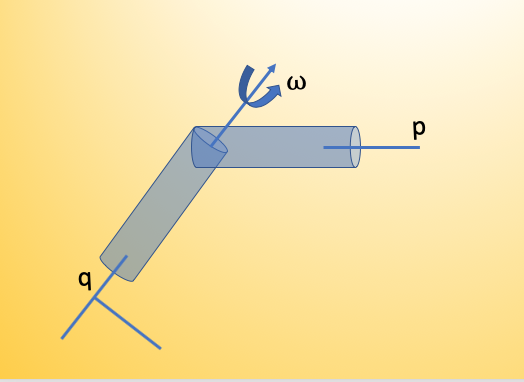
\includegraphics[width=.6\columnwidth]{figures/revolute.png}
	\caption{Illustration of rotation of interconnecting link of two spherical links.}
	\label{fig:revolute_point}
\end{figure}
%
In particular, we define the \textit{homogeneous coordinates} for a point $q \in \bb{R}^3$ that is rotating about an axis $\overrightarrow{\omega} \in \bb{R}^3$ such that $\|\overrightarrow{\omega}\| = 1$ (see \autoref{fig:revolute_point}) as 
%
\begin{align}
\hat{\xi} = \homo^{-1} \dot{\homo} = \left(\begin{array}{cc}
\hat{\omega} & v \\
%
0 & 0
\end{array}\right) \in \mathfrak{se}(3)
\label{eq:twist_defo}
\end{align}
%
where $v = -\omega \times q$. Equation \eqref{eq:twist_defo} is the object's velocity in the body frame; essentially the \textit{Lie algebra element} and we can obtain the twist coordinates from it via the so-called \textit{wedge operator} 
%
\begin{align}
\left(\begin{array}{c}
\hat{\omega} 
\\ 
v 
\end{array}\right)^{\wedge} = \left(\begin{array}{cc}
\hat{\omega} & v \\
%
0 & 0
\end{array}\right).
\end{align}
%
If the link of \autoref{fig:revolute_point} moves at a unit velocity, we can write the velocity at the tip point as 
%
\begin{align}
\dot{p} = \omega \times (p(t) - q(t)) 
\end{align}
%
where $p(t), q(t)$ are the paths traced out by points $p$ and $q$ respectively during the motion.
%

We define the exponential for  the matrix $A\in SO(n)$, which is a component of the solution to the ordinary differential equation, $\dot{x}(t) = A x(t)$ where $x(t) \in \bb{R}^n$ as 
%
\begin{tcolorbox}[title=The Matrix Exponential]
\begin{align}
e^{At} = \identity +  At + \dfrac{A^2t^2}{2!} + \dfrac{A^3 t^3}{3!} + \ldots 
\label{eq:matrix_exponential}
\end{align} 
\end{tcolorbox}
%

For the matrix exponential  of \eqref{eq:matrix_exponential}, we would like to write the equation in a closed-form expression since we are interested in definite solutions for our forward kinematics problems. For suppose that some matrix $D \in \bb{R}^{n\times n}$ and $P\in \bb{R}^{n\times n}$ are available, then we find that 
%
\begin{align}
e^{At} &= \identity + (PDP^{-1})t  + (PDP^{-1})(PDP^{-1})\dfrac{t^2}{2!}  + \ldots \nonumber \\
& = P\left(\identity  Dt + \dfrac{(Dt)^2}{2!} + \ldots \right)P^{-1} \\
& = P e^{Dt}P^{-1}.
\end{align}
%
\begin{definition}[Exponential Map Properties]
	%
	We note the following properties of the matrix exponential:
	
	\begin{inparaenum}
		\noindent(1) $d(e^{At}) = Ae^{At} = e^{At} A$.\\
		%
		(2) For $A=PDP^{-1}$ for some diagonal $D\in \bb{R}^{n\times n}$ and an invertible $P\in \bb{R}^{n\times n}, \,e^{At}=P e^{Dt}P^{-1}$.\\
		%
		(3) For $AB = BA$, we have $e^Ae^B = e^{A+B}$. \\
		%
		(4) $(e^A)^{-1} = e^{-A}$
		%
	\end{inparaenum}
	\label{def:exp_map}
\end{definition}
%

For the mapping from the twist map in the Lie algebra to the Lie group notation, we have the following:
%
\begin{tcolorbox}[title=Exponential map from $\mathfrak{se}(3)$ to $SE(3)$]
	\begin{align}
	e^{\hat{\xi \theta}} = \left(\begin{array}{cc}
	e^{\hat{\omega \theta}} & (\identity - e^{\hat{\omega} \theta}) (w \times v) + \omega \omega^T v \theta\\
	%
	0 & \identity
	\end{array}\right) \in SE(3)
	\end{align}
\end{tcolorbox}
%



\subsection{The Lie Group Notations}
\begin{figure}[tbph]
	\centering
	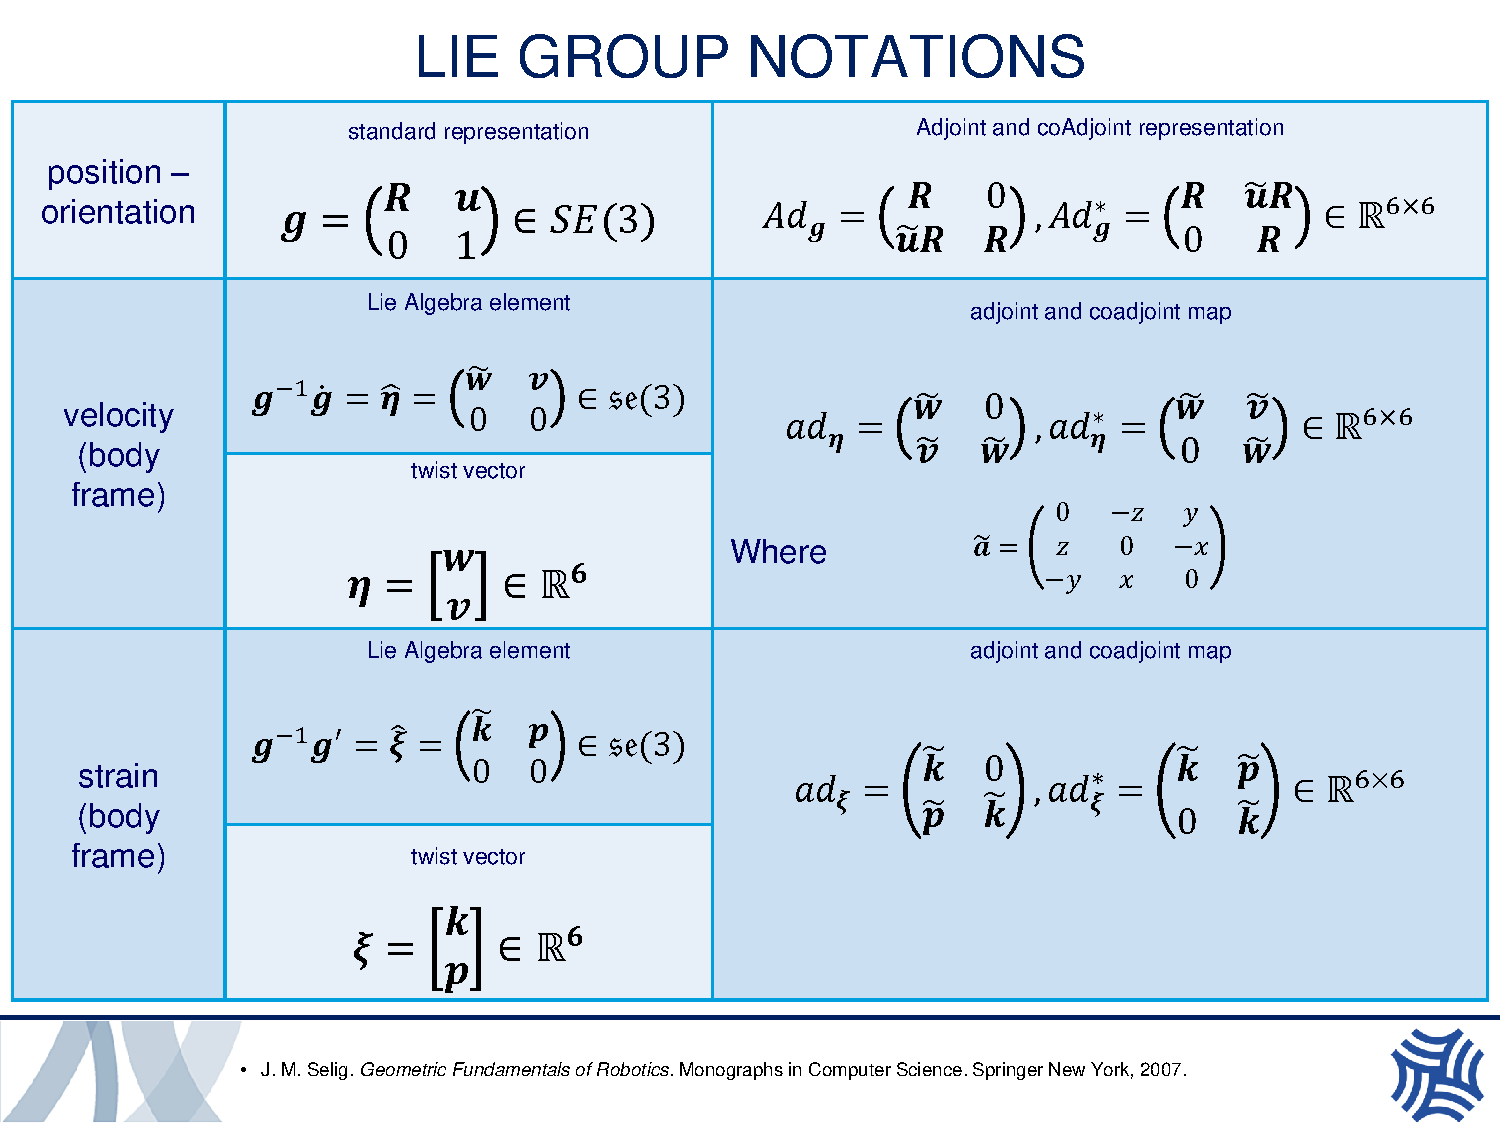
\includegraphics[width=\columnwidth]{figures/lienotations.pdf}
	\caption{Lie Group and their Notations. Reprinted with permission from Federico Renda. IROS 2018, Screw Theory Tutorial.}
	\label{fig:lienotations}
\end{figure}

\subsection{Exponential Map and Kinematic Chains}
\label{subsec:matexp}

Now consider a robot manipulator of the form shown in \autoref{fig:staubli}. The reader may imagine that there are right-handed triads of orthogonal vectors at the tip of each link of the chain so that the Euclidean transformation that describes the position and orientation of the $(i+1)'th$ link with the $i'th$ link is 
%
\begin{align}
\left(\begin{array}{cc}
\rot_i & \disp_i \\
0 & 1
\end{array}\right) \text{ exp } \left(\begin{array}{cc}
\skew_i & 0 \\
0 & 0
\end{array}\right)  \theta_i =  \homo_i \text{ exp } (\hat{\omega_i} \theta_i)
\end{align}
%
and we may imagine the triad that is fixed at the end-effector to be related to the triad at the base of the robot by the following relation
%
\begin{align}
H(\theta_1, \theta_2, \cdots, \theta_n) = \rot_1\,e^{\theta_1 \hat{\omega}_1}\,
%
\rot_2\,e^{\theta_2 \hat{\omega}_2},\, \cdots, 
%
\rot_n\,e^{\theta_n \hat{\omega}_n}\,	
\end{align}
%
and since $P exp(M) P^{-1} = exp(PMP^{-1})$, we can write the \textit{forward kinematic map}, $g_{st}: Q \rightarrow SE(3)$ as 
%
\begin{figure}[t!]
	\centering
	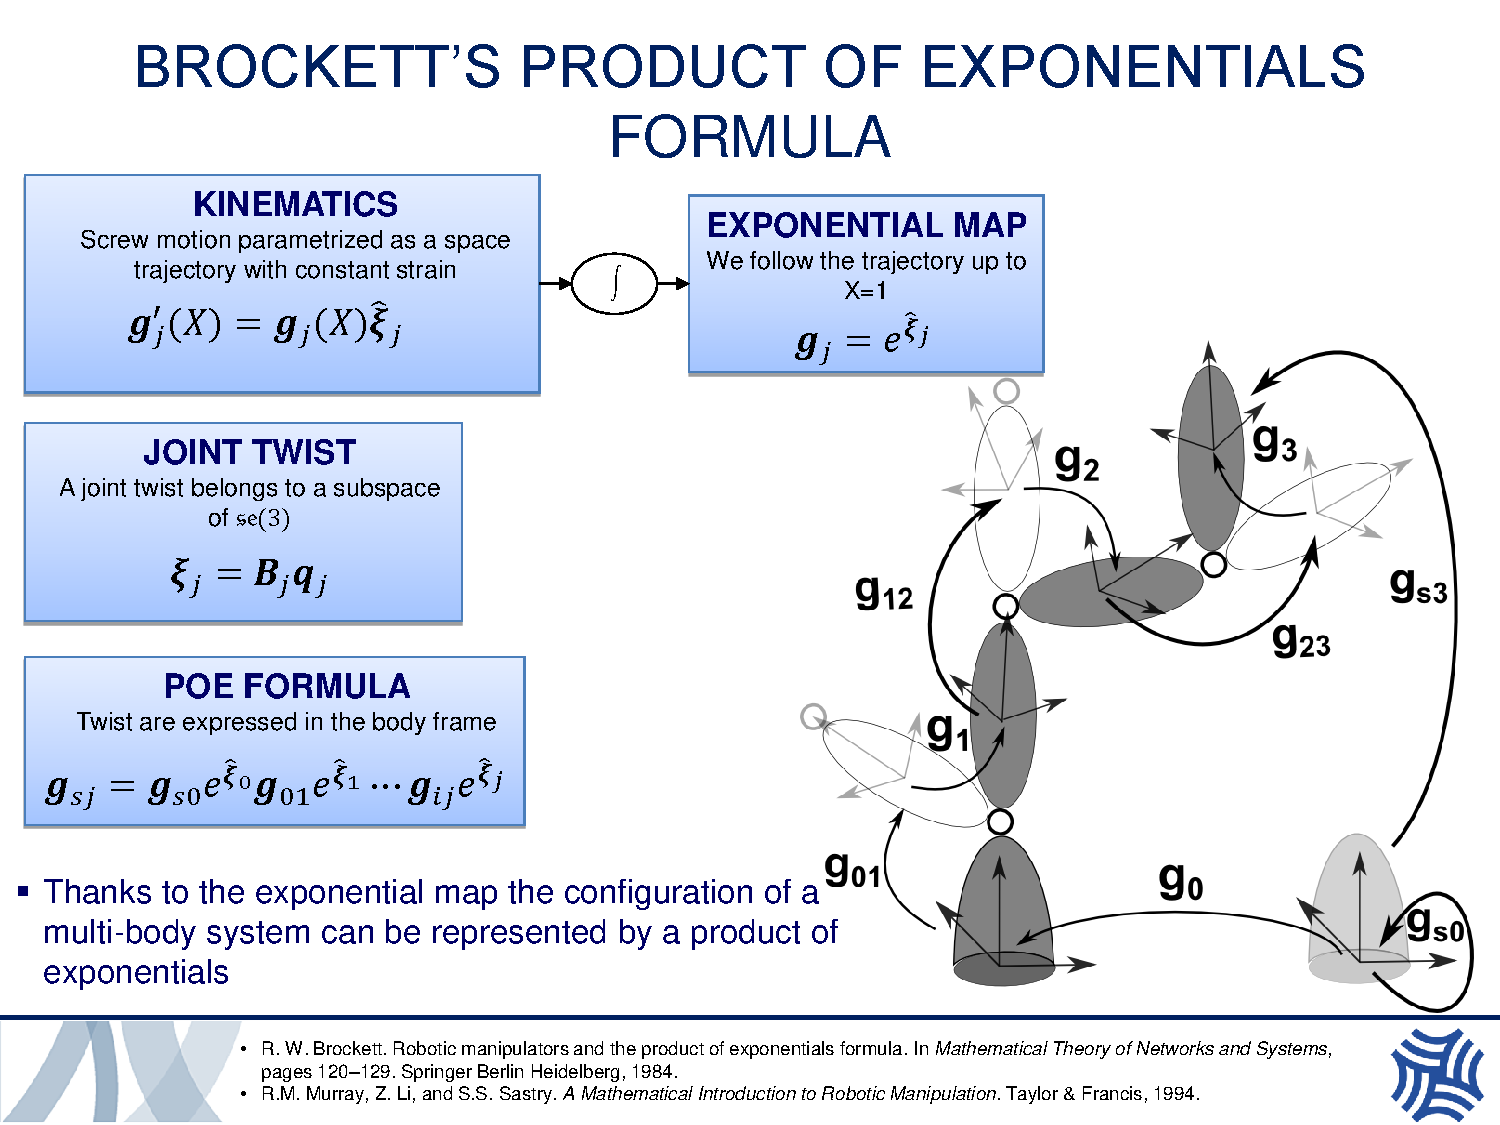
\includegraphics[width=\columnwidth]{figures/brockettpoe.pdf}
	\caption{An illustration of the exponential map for a multi-body rigid system. Reprinted with permission from Federico Renda. IROS 2018, Screw Theory Tutorial.}
	\label{fig:brockettpoe}
\end{figure}
%
\begin{align}
g_{st}(\theta) = e^{\theta_1 \hat{\omega}_1}\,
%
\,e^{\theta_2 \hat{\omega}_2}\, \cdots, 
%
\,e^{\theta_n \hat{\omega}_n}\,g_{st}(0)
\end{align}
%
using the identity repeatedly.
%
\section{Rigid Body Transformations}

A rigid body motion is one that preserves the  distance between points. In classical mechanics, we are concerned about the material description of a rigid body whereby we consider all the particles that make up the rigid body as a whole rather than treat them as a continuum as it is typical in continuum mechanics.  Therefore by this logic, \textit{a rigid body is a collection of particles by which the distance between any two particles remain fixed, irrespective of the motions of the body or forces exerted on that body~\cite{MurrayBook}}. 

Suppose we have two points $a$ and $b$ on a rigid body, we must have
%
\begin{align}
\|a(t_f) - b(t_f)\| = \|a(t_i) - b(t_i)\|
\end{align}
%
where $t_i$ and $t_f$ are two instants of time that the two points \ie $a$ and $b$ are observed on the rigid body. We thus see that distance is preserved irrespective of observer placement in rigid body transformations. For continuum-based systems such as soft robots, this is not so and we often need to come up with clever mechanisms of characterizing the motion of its particles. 

\noindent \textbf{Definition}: A mapping $g: \bb{R}^3\rightarrow\bb{R}^3$ is a \textit{rigid body transformation} if it satisfies the following properties:
\begin{itemize}
	\item Length is preserved \ie $\|g(a) - g(b)\| = \|a-b\|$ for all point $a, b \in \bb{R}^3$.
	%
	\item The cross product for all vectors is preserved \ie $g(p \times q) = g(p) \times g(q)$ where $p, q \in \bb{R}^3$ .
\end{itemize}
%
This means that the inner product is preserved so that we have, 
\begin{align}
p^Tq = g(p)^T \times g(q).
\end{align}
%
It follows that orthogonal vectors are transformed to orthogonal vectors and since cross product is naturally preserved, rigid body transformations map orthonormal coordinate frames to orthonormal coordinate frames. Note that it is possible to have rotation of particles despite the two strong forms presented above. To track the location of a rigid body in space, it therefore follows that we need to keep track of the motion of any one point as well as the rotation of the rigid body about this point. Therefore, the \textit{configuration} of the rigid body is found by attaching a Cartesian coordinate frame to a point on the rigid body and keeping track of the motion of the body coordinate frame with respect to a fixed frame. To ease representation, we typically require that all coordinate frames be \textit{right-handed}: given three Cartesian orthonormal vectors $\bm{x}, \bm{y}, \bm{z} \in \bb{R}^3$ which characterize the motion of a coordinate frame, they must satisfy $\bm{z} = \bm{x} \times \bm{y}$.


Going by the definitions of twist in the foregoing, it follows that a twist is to a rigid body what a vector is to a point. They both express the relation needed to transfer an object from one given position to another. When a body twists at an instant, the screw about which it twists is referred to as the \textit{instantaneous screw}.

\subsection{Translation in $\bb{R}^3$}

%
For the two coordinate frames shown in  \autoref{fig:2_coords}, say we choose the $o_0x_0 y_0$ frame as the reference and the $o_1x_1y_1$ as the moving coordinate frame, the way we would characterize the translation motion of the the point $q$ would be to represent its translation from the reference frame by the Cartesian displacement along $x$ and $y$ so that we have 
\begin{figure}
	\centering
	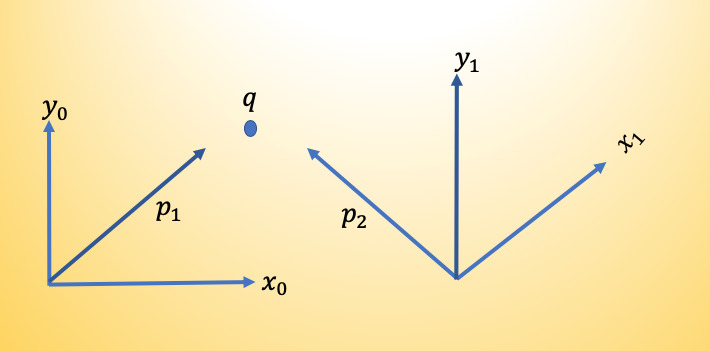
\includegraphics[width=.8\columnwidth]{figures/trans_coords.jpg}
	\caption{A point $q$ in space with respect to two coordinate frames.}
	\label{fig:2_coords}
\end{figure}
%
\begin{align}
q^0 = \left( \begin{array}{c}
q^0_x \\ q_y^0
\end{array}
\right), \quad
%
q^1 = \left( \begin{array}{c}
q^1_x \\ q_y^1
\end{array}
\right)
\end{align}
%
where the superscript denotes the reference frame and the subscript denotes the coordinate of the point $q$ along an axis in either Cartesian frame. The origin of the two frames are both points in space; therefore, the we can assign the coordinates that denote the position of the origin of one coordinate frame with respect to another as 
%
\begin{align}
o^0_1 = \left( \begin{array}{c}
o^0_x \\ o^0_y
\end{array}
\right), \quad
%
o^1_0 = \left( \begin{array}{c}
o^1_x \\ o^1_y
\end{array}
\right).
\end{align}
%
For vectors such as twists or wrenches, we use a similar notation as those used for points. Thus if $p_1, p_2$ are two vectors that are invariant with respect to the choice of coordinate frames, we would have
%
\begin{align}
p^0_1 = \left( \begin{array}{c}
o^0_x \\  o^0_y
\end{array}
\right)^T,
%
\quad p^1_1 = R(-\theta) q^0, 
%
\quad p^0_2 = R(\theta) q^0, \quad p^1_2 = \left( \begin{array}{c}
o^1_x \\  o^1_y
\end{array}
\right)^T
\end{align}
%
where $\theta$ is the angle that coordinate frame $1$ makes with respect to coordinate frame $0$. In robotics, the standard way to apply a rotation is counterclockwise. This is the reason we negate the angle of rotation when finding the vector $p_1$ in frame $1$. We will introduce the definition of the rotation matrix $R$ shortly. Performing frame transformations is a fundamental step to getting a robot work as envisioned. We must ensure that all coordinate vectors are defined with respect to the same coordinate frame. We say two vectors are ``equal" when they have the same magnitude and direction. Therefore, for vectors that are not constrained to be located at the same point in space, we require that they defined with respect to frames whose coordinates are parallel, given that absolute locations are not consequential, but the magnitude and direction of the vector.

\subsection{Rotations in $\bb{R}^3$}
%
We would like to establish a convention  that all coordinate frames will be right-handed. Our goal is to establish the orientation of an object by specifying the local coordinate on the body; we then describe the body's \textit{relative orientation} between a coordinate frame attached to the body and a fixed or an inertial coordinate frame. 
%
\begin{figure}[tb!]
	\centering
	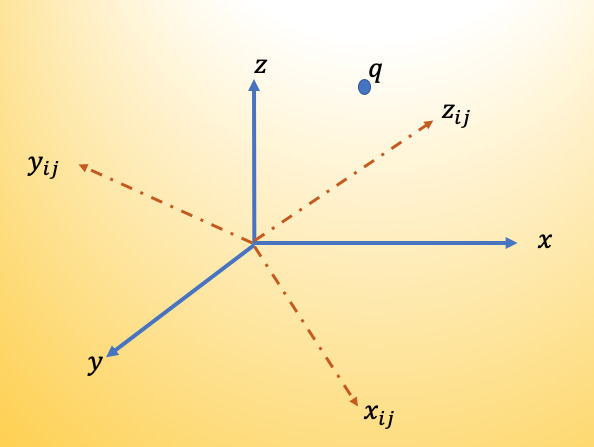
\includegraphics[width=\columnwidth]{figures/rotation_illus.jpg}
	\caption{An illustration of the relative orientation of a rigid object $q$ between an inertial frame $I$ and a body frame $J$.}
	\label{fig:rotation_illus}
\end{figure}
%
Suppose that we have two frames $I$ and $J$, where $I$ is the inertial frame, while $J$ is the body frame as shown in \autoref{fig:rotation_illus}. Let $\bm{x}_{ij}, \bm{y}_{ij},\bm{z}_{ij} \in \bb{R}^3$ be the coordinates of the principal axes of $J$ relative to $I$ so that we have the following matrix as a result of composing the respective coordinate vectors
%
\begin{align}
R_{ij} = \begin{bmatrix}
\bm{x}_{ij} \quad  \bm{y}_{ij} \quad \bm{z}_{ij}
\end{bmatrix} = \begin{bmatrix}
r_{11} &  r_{12} & r_{13} \\
r_{21} & r_{22} &  r_{23} \\
r_{31} & r_{32} &  r_{33}
\end{bmatrix}.
\label{eq:rotation_compoz}
\end{align}
%
The resulting matrix in \eqref{eq:rotation_compoz} is the \textit{rotation matrix}. This matrix can be rewritten by noting that the components of a vector are the projections of that vector onto the unit directions of its reference frame. Thus, the components if $R_{ij}$ in \eqref{eq:rotation_compoz} can be written as the dot product of a pair of unit vectors:
%
\begin{align}
R_{ij} = \begin{bmatrix}
\bm{x}_j \cdot \bm{x}_i & \bm{y}_j \cdot \bm{x}_i & \bm{z}_j \cdot \bm{x}_i \\
%
\bm{x}_j \cdot \bm{y}_i & \bm{y}_j \cdot \bm{y}_i & \bm{z}_j \cdot \bm{y}_i \\
%
\bm{x}_j \cdot \bm{z}_i & \bm{y}_j \cdot \bm{z}_i & \bm{z}_j \cdot \bm{z}_i 
\end{bmatrix}.
\label{eq:direction_cosines}
\end{align}
%
The components of the rotation matrix \eqref{eq:rotation_compoz} are sometimes called direction cosines since the dot product of two unit  vectors give the cosine of the angle between them as shown in \eqref{eq:direction_cosines}. If we examine the rows of \eqref{eq:direction_cosines}, we see that the rows of $R_{ij}$ are the unit vectors coordinates of $I$  in the frame $J$ so that we have 
%
\begin{align}
R_{ij} = R_{ji}^T
\end{align}
%
which is to say that the inverse of the rotation matrix is equal to its transpose. 
Noting that $\|\bm{r}\|^2 = x_i^2 + y_j^2+z_i^2 = 1$,  $r_i \cdot r_j = 0$ when $i \neq j$, and $r_i \cdot r_i = 0$, this can be thus verified as 
%
\begin{align}
R_{ij}^T \cdot R_{ji} & = 
\begin{bmatrix}
\bm{x}_j \cdot \bm{x}_i & \bm{x}_j \cdot \bm{y}_i  & \bm{x}_j \cdot \bm{z}_i \\
%
\bm{y}_j \cdot \bm{x}_i & \bm{y}_j \cdot \bm{y}_i & \bm{y}_j \cdot \bm{z}_i \\
%
\bm{z}_j \cdot \bm{x}_i & \bm{z}_j \cdot \bm{y}_i  & \bm{z}_j \cdot \bm{z}_i 
\end{bmatrix}
\cdot 
\begin{bmatrix}
\bm{x}_j \cdot \bm{x}_i & \bm{y}_j \cdot \bm{x}_i & \bm{z}_j \cdot \bm{x}_i \\
%
\bm{x}_j \cdot \bm{y}_i & \bm{y}_j \cdot \bm{y}_i & \bm{z}_j \cdot \bm{y}_i \\
%
\bm{x}_j \cdot \bm{z}_i & \bm{y}_j \cdot \bm{z}_i & \bm{z}_j \cdot \bm{z}_i 
\end{bmatrix} \\
%
& = 
\begin{bmatrix}
\bm{x}_j \cdot \bm{x}_j \cdot \|\bm{r}\|^2 & \bm{x}_j \cdot \bm{y}_j \cdot \|\bm{r}\|^2 & \bm{x}_j \cdot \bm{z}_j  \cdot \|\bm{r}\|^2  \\
%
\bm{y}_j \cdot \bm{x}_j  \cdot \|\bm{r}\|^2  & \bm{y}_j \cdot \bm{y}_j  \cdot \|\bm{r}\|^2  & \bm{y}_j \cdot \bm{z}_j  \cdot \|\bm{r}\|^2  \\
%
\bm{z}_j \cdot \bm{x}_j  \cdot \|\bm{r}\|^2  & \bm{z}_j \cdot \bm{y}_i  \cdot \|\bm{r}\|^2  & \bm{z}_j \cdot \bm{z}_j  \cdot \|\bm{r}\|^2  
\end{bmatrix}
%
= 
\left(\begin{array}{ccc}
1 & 0 & 0 \\
%
0 & 1 & 0  \\
%
0 & 0 & 1 
\end{array}\right) \\
%
& = \bm{I}_3
\end{align}
%
where $\bm{I}_3$ is the $3 \times 3$ identity matrix.
%

\noindent 
\begin{homework}
	Verify that $R_{ij} = R_{ji}^{-1} \equiv R_{ji}^T$. Furthermore, verify that the determinant of the rotation matrix is $\pm1$ \ie $det R = \pm1$.
\end{homework}

The determinant of the $R$ matrix is written as 
%
\begin{align}
\text{det }  R = r_1^T \left(r_2 \times r_3\right).
\end{align}
%
For right-handed coordinate frames, we have that $r_2 \times r_3 = r_1$ so that $r_1^Tr_1 = 1$ for a coordinate frame that aligns with the right-hand orthonormal frame representation. This special property that a $3 \times 3$ matrix satisfies $r_2 \times r_3 = r_1$ and that $\text{det }  R = r_1^Tr_1 = 1$ is called the special orthogonal property, denoted \textit{SO(3)}. Special orthogonal means $\text{det } R = + 1$. The set of all SO matrices in $\bb{R}^{n\times n}$ is defined by 
%
\begin{align}
SO(n) = \{R\in \bb{R}^{n\times n}: RR^T = \bm{I}, \text{det } R = + 1\}.
\end{align}

\subsection{Rotation Matrices as Transformations}
%
Suppose we are tasked with transforming a point $q$ from one coordinate frame  $J$ to a frame $I$ based on  \autoref{fig:rotation_illus}. Suppose that $q_j = (x_j, y_j, z_j)$ are the coordinates of $q$ with respect to the frame $J$. We may reason that $x_j, y_j, z_j \in \bb{R}^3$ are the projections of $q$ onto the coordinate axes of $J$, which in turn, have coordinates $\bm{x}_{ij}, \bm{y}_{ij},\bm{z}_{ij} \in \bb{R}^3$ with respect to coordinate frame $I$; then it follows that the coordinates of $q$ relative to frame $I$ is
%
\begin{align}
q_i = \bm{x}_{ij} x_j + \bm{y}_{ij} y_j + \bm{z}_{ij} z_j.
\end{align}
%
which in vectorized form is 
%
\begin{align}
q_i & = \left(\begin{array}{ccc}
\bm{x}_{ij} &  \bm{y}_{ij} & \bm{z}_{ij}
\end{array}\right)
%
\left(\begin{array}{c}
x_j \\ y_j \\ z_j
\end{array} \right) 
& = R_{ij}q_j
\end{align}
%
where the last part of the above equation follows from \eqref{eq:direction_cosines}.

Just as a rotation matrix can act on points to transform them in the world, so can rotation matrices act on vectors. Say we have another point $p_j$ on the frame $J$ in \autoref{fig:rotation_illus}, then the vector that connects a point $q_j$ in the frame $J$ to $p_j$ is $v_j = q_j - p_j$ so that the action of the rotation matrix on $v_j$ is
%
\begin{align}
R_{ij}(v_j) := R_{ij} q_j - R_{ij} p_j = q_i - p_i = v_i.
\end{align}


\subsection{Planar Rotations}
%
We now revisit the relative orientation between two coordinate frames as shown in \autoref{fig:rotation_illus}. Suppose now that the angle of rotation between the two coordinate frames is $\theta$ as shown in \autoref{fig:planar_rot}, it follows that 
%
\begin{figure}[tb!]
	\centering
	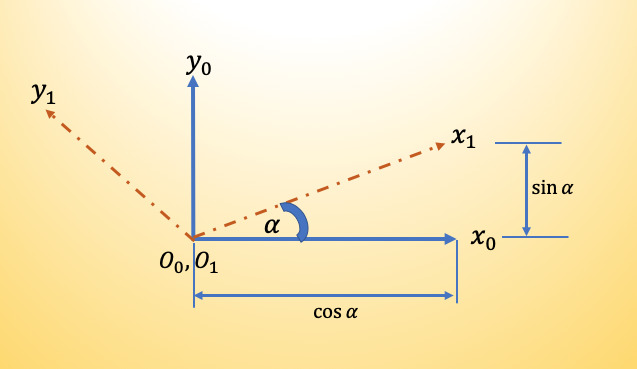
\includegraphics[width=.75\columnwidth]{figures/planar_rot.jpg}
	\caption{Illustration of rotation between two frames in a plane.}
	\label{fig:planar_rot}
\end{figure}
%
the composition of the rotation allows us to write 
%
\begin{align}
R_1^0 = \left(\begin{array}{cc}
x_1^0 \,\,| & y_1^0
\end{array}\right)
\end{align}
%
whereupon $x_1^0$ and $y_1^0$ have the usual meanings as before and are expressed as 
%
\begin{align}
x_1^0 = \left(\begin{array}{cc}
\cos \alpha \\ \sin \alpha
\end{array}\right) \text{ and }
%
y_1^0 = \left(\begin{array}{cc}
-\sin \alpha \\ \cos \alpha
\end{array}\right)
\end{align}
%
so that composing the rotation matrix, we have
%
\begin{align}
R = \left(\begin{array}{cc}
\cos \alpha & -\sin \alpha \\ \sin \alpha &  \cos \alpha
\end{array}\right)
\end{align}
%
While you might find the above approach rather daunting, an easier geometric way to visualize the transformation of matrices is to recall that the columns of the rotation matrix are the direction cosines of the coordinate axes of $o_1x_1y_1$ relative to the coordinates of $o_0x_0y_0$ \cf \eqref{eq:direction_cosines}. For a planar rotation, we could extract the first $2\times 2$ block of \eqref{eq:direction_cosines} so that 
%
\begin{align}
R_1^0 = \begin{bmatrix}
\bm{x}_0 \cdot \bm{x}_1 & \bm{y}_1 \cdot \bm{x}_0 \\
%
\bm{x}_0 \cdot \bm{y}_1 & \bm{y}_1 \cdot \bm{y}_0
\end{bmatrix} 
\end{align}
%
And since the dot product of two vectors is basically the cosine of the angles between them, we have
%
\begin{align}
R_1^0 =  \begin{bmatrix}
cos \alpha &  -cos(\pi/2 - \alpha) \\
%
cos(\pi/2 - \alpha) & cos \alpha
\end{bmatrix} 
%
=  \begin{bmatrix}
cos \alpha &   - \sin \alpha  \\
%
\sin \alpha  & cos \alpha
\end{bmatrix} 
\end{align}
%
Note the way the negative signs have entered the matrix due to the counterclockwise direction of rotation that we have chosen so as to preserve the positiveness of the determinant of $R$. In particular, the projection of $y_1$ on $x_0$ is negative because of our right-handed frame.

\noindent 
\begin{homework}
	Compose the rotation matrix in three dimensions where all axes of the inertial frame are rotated by an angle $\beta$ around each of the $x_0$, $y_0$ and $z_0$ axes respectively using the foregoing logic. In addition, for each transformation, verify that (1) $R_{e, \beta} = I$ where $e$ is the axes about which we are rotating and $\beta$ is the angle of rotation, (2) the composition of rotations about the angles $\beta$ and $\alpha$ in a successive manner implies that $R_{z, \beta}, R_{z, \alpha} = R_{z, \beta + \alpha}$, and (3) ${(R_{z, \beta})}^{-1} = R_{z, -\beta}$. Bonus points will be awarded for cool 3D visualizations.
\end{homework} 

\begin{figure}[tb!]
	\centering
	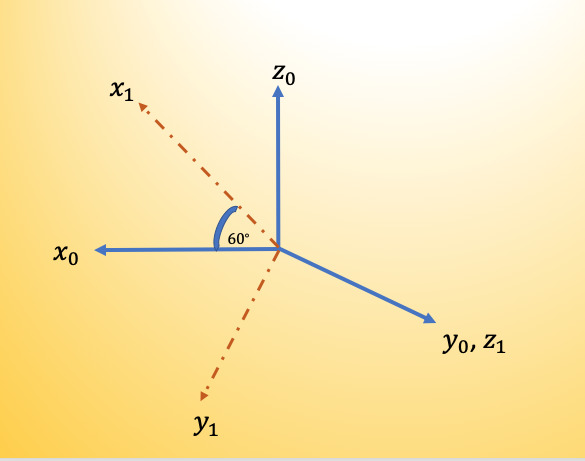
\includegraphics[width=.8\columnwidth]{figures/two_frames.jpg}
	\caption{Relative orientation between two frames.}
	\label{fig:two_frames}
\end{figure}


\noindent 
\begin{homework}
	For the two frames shown in \autoref{fig:two_frames}, determine the rotation matrix between them. In addition, explain the difference between rotating about a \textit{current frame} and rotating about a \textit{fixed frame}\footnote{See sections 2.4.1 and 2.4.2 of Spong's book.}. In particular, when is it necessary to carry out a \textit{pre-multiplication} and when is it necessary to carry out a \textit{post-multiplication} when transforming points or vectors about coordinate frames?
\end{homework}

\begin{tcolorbox}[title=Order of rotations]
	%
	A rotation about a fixed axis necessarily means a \textbf{pre-multiplication} while a rotation about a current axis necessitates a \textit{post-multiplication}.
\end{tcolorbox}


\subsection{Composition of Rotations}
%
Rotations matrices have this desirable property that they can be composed together to form transform a point between successive frames. Take for example a frame $K$ whose orientation relative to frame $J$ is $R_{jk}$, and frame $J$ whose orientation relative to frame $I$ is $R_{ij}$, we can write out the orientation of frame $K$ relative to $I$ as 
%
\begin{align}
R_{ik} = R_{ij} R_{jk}.
\label{eq:current_frame_rotation}
\end{align}
%
The rotation described above would be equivalent to rotating frame $J$ relative to frame $I$ according to $R_{ij}$, then aligning frame $J$  to $K$, we rotate $K$ relative to $I$ according to $R_{jk}$. The resulting frame $K$ has orientation with respect to $I$ given by $R_{ij} R_{jk}$. This frame relative to which rotation occurs is termed the \textit{current frame}.

\noindent 
\begin{homework}
	For the robot manipulator we are using in this class, suppose that you have the following point in the base frame of the robot, $q_o = [-2, 3, 1]$. Furthermore, suppose that the joint angles for all six joints are respectively $\{-90, 60, 30, 45, 90, 125 \}$, transform the point $q_0$ in the base frame to a coordinate frame on the sixth joint.
\end{homework}

%
\begin{tcolorbox}[title=Properties of Rigid Body Rotation Matrices]
	\textit{Rigid body} rotations preserve
	\begin{itemize}
		\item distance: $\|Rq - Rp\| = \|q-p\|$ for all $q, p \in R^3$
		%
		\item orientations: $R(i \times j) = Ri \times Rj$ for all $i, j \in \bb{R}^3$.
	\end{itemize}
\end{tcolorbox}

What follows is adapted from Figure 2.5 from Spong and Vidyasagar's book. It is meant to illustrate the rotation applied to a point from one frame to another.
%
\begin{figure}[tb!]
	\centering
	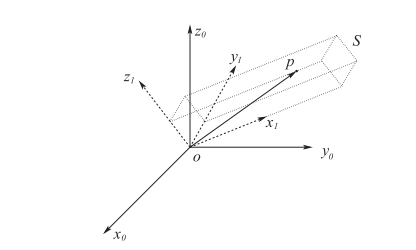
\includegraphics[width=.8\columnwidth]{figures/point_transform.png}
	\caption{Coordinate frames on a body. Reprinted from \cite{SpongBook}}.
	\label{fig:point_transform}
\end{figure}

For consider \autoref{fig:point_transform} whereupon the rigid body $S$ has a coordinate frame $o_1x_1y_1$ attached. For the coordinates of the point p with respect to frame $o_1x_1y_1$ or $p^1$, we are tasked with finding the coordinates of $p$ relative to a fixed reference frame $o_0x_0y_0$. We note that $p^1 = [u, v, w]^T$ satisfies 
%
\begin{align}
p = ux_1 + v y_1 + w z_1.
\label{eq:point_transform1}
\end{align}
%
Matter-of-factly, the coordinates of $p^0$ can be obtained based on the projection trick we introduced earlier by projecting $p$ onto the coordinate axes of $o_0x_0y_0z_0$ so that we have 
%
\begin{align}
p^0 = \left(\begin{array}{c}
p \cdot x_0 \\ p \cdot y_0 \\ p \cdot z_0
\end{array}\right)
\label{eq:point_transform2}
\end{align}
%
so that substituting \eqref{eq:point_transform1} into \eqref{eq:point_transform2}, we have
%
\begin{align}
p^0 = \left(\begin{array}{c}
(ux_1 + v y_1 + w z_1) \cdot x_0 \\ (ux_1 + v y_1 + w z_1) \cdot y_0 \\ (ux_1 + v y_1 + w z_1)  \cdot z_0
\end{array}\right)
%
= \left(\begin{array}{ccc}
x_1 \cdot x_0 & y_1 \cdot x_0 & z_1 \cdot x_0 \\
%
x_1 \cdot y_0 &  y_1 \cdot y_0 &  z_1 \cdot y_0\\ 
%
x_1  \cdot z_0 &  z_1  \cdot z_0 &  z_1  \cdot z_0
\end{array}\right) \left(\begin{array}{c}
u \\ v \\ w
\end{array}\right)
\label{eq:point_transform3}
\end{align}
%
which upon inspection turns out to be a multiplication of the rotation matrix that transforms point $p^1$ to point $p^0$ \ie
%
\begin{align}
p^0 = R_1^0 p^1,
\end{align}
%
implying that the rotation matrix not only serves to represent the relative orientation of coordinate frames with respect to one another but to transform coordinates of a point from one frame to another.

Finally, we define a similarity transformation \textit{as the matrix representation of a general linear transformation that is transformed from one frame to another}. So if $I$ is the matrix representation of a linear transformation in a frame $o_0x_0y_0z_0$ and $J$ is the equivalent transformation in $o_1x_1y_1z_1$ then $I$ and $J$ are related by 
%
\begin{align}
J = (R_1^0)^{-1}AR_1^0
\end{align}
%
where $R_1^0$ is the coordinate transformation between frames $o_1x_1y_1z_1$ and $o_0x_0y_0z_0$.

\noindent \textbf{Lab Exercise}: Carry out a similarity transformation in the elbow frame ($o_1x_1y_1z_1$) of the manipulator with respect to the shoulder frame ($o_0x_0y_0z_0$) when the two frames are related by the rotation 
%
\begin{align}
R = 	\left(\begin{array}{ccc}
1 & 0 & 0 \\
%
0 & -1 & 0 \\
%
0 & 0 & 0
\end{array}\right)
\end{align}
%

Consider the composition of rotations of \autoref{fig:compoz} where we first rotate by an angle $\theta$ about the $x$ axis and then rotate about an angle $\psi$ about the $z$ axis. The rotation matrix can be composed as 
%
\begin{figure}[tb!]
	\centering
	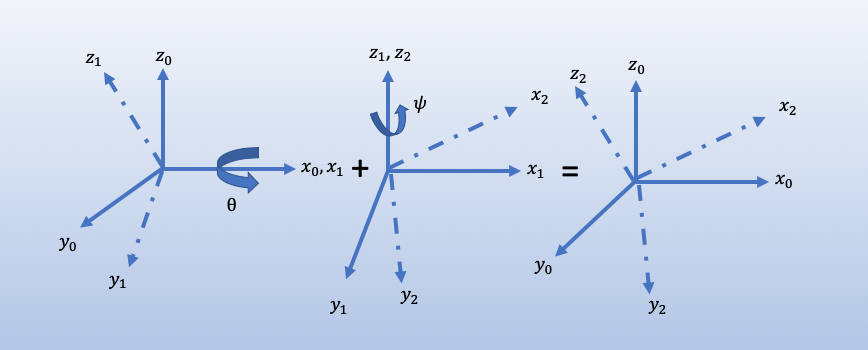
\includegraphics[width=\columnwidth]{figures/compoz.png}
	\caption{Illustration of composition of rotations about a \textbf{current axis}.}
	\label{fig:compoz}
\end{figure}
%
\begin{align}
R &= R_{x, \theta} R_{z, \psi} 
%
&= \left(\begin{array}{ccc}
1 & 0 & 0 \\
0 & c_\theta & -s_\theta \\
0 & s_\theta & c_\theta
\end{array}\right) 
%
\cdot
%
\left(\begin{array}{ccc}
c_\psi & -s_\psi & 0 \\
s_\psi & c_\psi & 0 \\
0 & 0 & 1
\end{array}\right)
%
&= \left(\begin{array}{ccc}
c_\psi & -s_\psi & 0 \\
0 & c_\theta c_\psi &  -s_\theta \\
s_\theta s_\psi & s_\theta c_\psi & c_\theta 
\end{array}\right)
\end{align}
%
Notice how the order of multiplication is carried out, owing to the axis about which we are making the transformation. 

\noindent 
\begin{homework}
	Carry out the transformation above in reverse order. What do you notice?
\end{homework} 


\section{Parameterization of Rotations $\in SO(3)$}
%
\subsection{Axis-Angle Parameterizations}
The exponential coordinates are the \textit{canonical} coordinates of the rotation group. A rigid body has at most three rotational degrees of freedom so that we need at most three variables to denote its orientation in the world. For the matrix 
%
\begin{align}
	R = \begin{bmatrix}
	r_{11} & r_{12} & r_{13} \\
	%
	r_{21} & r_{22} & r_{23} \\
	%
	r_{31} & r_{32} & r_{33} \\
	\end{bmatrix}
\end{align}
%
so that equating the foregoing with the exponential map for a rotation about $\theta$ around an axis $\omega$ as yields
%
\begin{align}
	e^{\hat{\omega}\theta}  &= \identity + \hat{\omega} \sin \theta + \hat{\omega}^2(1 - \cos \theta) \\%
	%
	& = \begin{bmatrix}
	\omega_y^2 v_\theta + c_\theta  & \omega_x\omega_y v_\theta - \omega_z s_\theta & \omega_x \omega_z v_\theta + \omega_y \, s_\theta \\
	 %
	\omega_x \omega_y v_\theta + \omega_z s_\theta  & \omega_y^2 v_\theta+ c_\theta & \omega_y \omega_z v_\theta - \omega_x s_\theta \\
	%
	\omega_x \omega_z v_\theta - \omega_y s_\theta  & \omega_y \omega_z v_\theta + \omega_x s_\theta & \omega_z^2 v_\theta + c_\theta
	\end{bmatrix},
	\label{eq:axis_angle}
\end{align}
%
where we have used $v_\theta = 1 - \cos \theta$. Therefore, we have
%
\begin{align}
	trace(R) = r_{11}  + r_{22}  + r_{33} = 1 + 2 c_\theta
\end{align}
%
Inspecting the matrix of \eqref{eq:axis_angle}, we have the angle of rotation in terms of the three components of the rotation matrix as 
%
\begin{align}
	\theta = \cos^{-1}\left(\dfrac{trace(R) -1}{2}\right)
	\label{eq:angle_part}
\end{align}
% 
where $\theta$ is defined under the constraint, $-2\pi n \le \theta \le 2 \pi n$  owing to the special property of $R$.\footnote{Since $R$ preserves lengths and $\text{ det } R = + 1$, the eigenvalues of R have a unit magnitude and occur in complex conjugate pairs. This implies $-1 \le trace(R) \le 3$}. 

\noindent 
\begin{homework}
	Verify by equating the off-diagonal terms that 
	%
	\begin{align}
	\omega = \frac{1}{2 \sin \theta} \left(
	\begin{array}{c}
	r_{32} - r_{23} \\
	%
	r_{13} - r_{31} \\
	%
	r_{21} - r_{12}
	\end{array} \right)
	\label{eq:axis_part}
	\end{align}
	%
	\noindent suppose $\theta \neq 0$. 
	Equation \eqref{eq:angle_part} together with \eqref{eq:axis_part} are what we call the \textit{axis-angle representation}.
\end{homework} 
%

\subsection{Euler Angles}
%
The \textit{Euler Angles} are particularly useful for specifying the orientation of a a coordinate frame $J$ with respect to $I$. To do this, we start as follows (see \autoref{fig:zyz} for reference):
%
\begin{figure}[tb!]
	\centering
	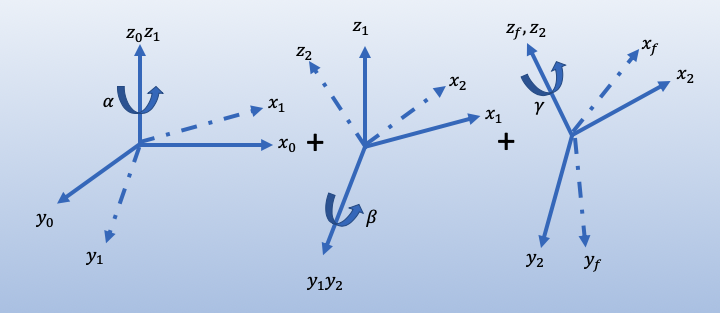
\includegraphics[width=.8\columnwidth]{figures/zyz.png}
	\caption{An illustration of the ZYZ rotation angles}
	\label{fig:zyz}
\end{figure}
\begin{itemize}
	\item we orientate frame $J$ with frame $I$ so that the two frames are coincident by rotating by the $z$ axis about an angle $\alpha$;
	%
	\item we then rotate about the \textit{new} y-axis of $J$ by an angle $\beta$;
	%
	\item lastly, we rotate about the new z-axis of rge frame $J$ by an angle $\gamma$ 
\end{itemize}
%
so that altogether, we have a rotation $R_{ij}(\alpha, \beta, \gamma)$ given as 
%
\begin{align}
	R_{ij}(\alpha, \beta, \gamma) &= R_z(\alpha) R_y(\beta) R_z(\gamma) \\
	%
	& = \begin{bmatrix}
	c_\alpha & -s_\alpha & 0 \\
	%
	s_\alpha & c_\alpha & 0 \\
	%
	0 & 0 & 1
	\end{bmatrix}
	%
	\begin{bmatrix}
	c_\theta  & 0 & s_\theta\\
	%
	0  & 1 & 0 \\
	%
	-s_\theta  & 0 & c_\theta 
	\end{bmatrix} \nonumber \\
	%
	&= \begin{bmatrix}
	c_\alpha c_\beta c_\gamma - s_\alpha s_\gamma & -c_\alpha c_\beta s_\gamma - s_\alpha c_\gamma & c_\alpha s_\beta \\
	%
	s_\alpha c_\beta c_\gamma + c_\alpha s_\gamma & -s_\alpha c_\beta s_\gamma + c_\alpha c_\gamma  & s_\alpha s_\beta \\
	%
	-s_\beta c_\gamma & s_\beta s_\gamma & c_\beta
	\end{bmatrix} 
	\label{eq:zyz}
\end{align}
%
where as before the abbreviations $c_\alpha, s_\alpha$ are abbreviations for $\cos \alpha$ and $\sin \alpha$. Euler angles arise when we need to recover the $\alpha, \beta, \gamma$ angles from \eqref{eq:zyz}. Suppose that $r_{13}$ and $r_{23}$ are both  $\neq 0$, we find that $c_\beta \neq \pm 1$ and thus with the knowledge that $\sin \beta >0$ given \eqref{eq:euler_a}, we find that , 
%
\begin{subequations}
\begin{align}
\beta &= \arctan 2(r_{33}, \sqrt{1 - r_{33}^2})  \label{eq:euler_a}\\
\alpha &= \arctan 2(r_{23}/\sin \beta, r_{13}/\sin \beta) \label{eq:euler_b} \\
\gamma &= \arctan 2 (r_{32}/\sin \beta, -r_{31}/\sin \beta)
\end{align}
\label{eq:euler}
\end{subequations}
%
where $\arctan2(y, x)$ computes $\tan^{-1}(y/x)$, determining the quadrant of the angle based on the sign of $x$ and $y$.
%
When $\sin \beta < 0$, we find that 
%
\begin{subequations}
	\begin{align}
	\beta &=  \arctan2(r_{33}, -\sqrt{1 - r_{33}^2})  \label{eq:euler_neg_a}\\
	\alpha &= \arctan 2(-r_{23}/\sin \beta, -r_{13}/\sin \beta) \label{eq:euler_neg_b} \\
	\gamma &= \arctan 2 (-r_{32}/\sin \beta, r_{31}/\sin \beta)
	\end{align}
	\label{eq:euler_neg}
\end{subequations}
%
implying that \textit{the Euler angles are not unique} owing to the sign of the angle about which the $y$ axis rotates. 

\noindent 
\begin{homework}
	What happens when $r_{13} = r_{23} = 0$? Can you write out the rotation matrix as well as the euler angles for this situation?
\end{homework}

In the scenario that results from homework viii, there will be infinitely many solution owing to the fact that only $\alpha + \beta$ only can be determined. This infinite solutions occur wehn $\rot = \identity$ and an example scenario of when this occurs is when $(\alpha, 0, -\alpha)$.

Using the $ZYZ$ angles are not the only way of parameterizing the rotation matrix. We could permute the order of rotation or rotate successively about different axis. Examples include $ZYX$ axes rotations (or Fick angles) and the $YZX$ axes parameterization or Helmholtz angles. In general robotics speak, note that the \textit{$ZYX$  angles are otherwise referred to as the yaw, pitch and roll angles, wherein the rotation matrix $\rot_{ij}$ is defined by rotating about the $x-$axis in the body frame (roll), then the $y-$axis in the body frame (pitch), and finally the $z-$axis in the body frame (yaw). } An advantage of the Fick angle  and Helmholtz angle parameterization is that they avoid singularity at $\rot = \identity$ though they do contain singularities at other configurations.

\subsection{Quaternions}
%
Rather than use rotation matrices to represent orientations, a more effective approach of representing orientations are \textit{quaternions}. Intead of locally parameterizing the \textit{SO(3)} Lie group, quaternions, unlike rotation matrices, globally parameterize the \textit{SO(3)} Lie Group. Formally, we represent a quaternion as follows:
%
\begin{align}
	Q = q_0 + q_x \bm{i} + q_y \bm{j} + q_z \bm{k} , \quad {q_i}_{\{i = 0, \cdots, 3\}} \in \bb{R}
\end{align}
%
where $q_0$ is the scalar component of $Q$ and $\bm{q} = (q_x, q_y, q_z)$ is the vector component.

The \textit{unit quaternions} are the subset of all $Q \in \bb{Q}$ such that $\|Q\| = 1$; for a rotation matrix $R = \text{exp}(\hat{\omega}\theta)$, we have the unit quaternion as 
%
\begin{align}
	Q = \left(\cos(\theta/2), \omega \sin \left(\theta/2\right) \right),
\end{align}
%
where $\omega \in \bb{R}^3$ is the axis of orientation and $\theta \in \bb{R}$ is the angle of rotation.

\begin{tcolorbox}[title=Summary of Parameterizations]
	Rotation matrices can be parameterized in one of many ways depending on our use case. The common examples of parameterizations are 
	%
	\begin{inparaenum}[\itshape (1)\upshape] \newline
		\item Axis-Angle representation; \newline
		\item Euler  angles ($ZYZ$) representation; \newline
		\item Fick  angles (\ie $ZYX$ or yaw, pitch and roll)  representation; \newline
		\item Helmholtz angles (or $YZX$) angles representation; and \newline
		\item Quaternions.
	\end{inparaenum}
	
\end{tcolorbox}

\section{Homogeneous Coordinates}
%
For a point $q \in \bb{R}^3$, we represent the \textit{homogeneous coordinates} of point $q$ as 
%
\begin{align}
	\bar{q} = \left(\begin{array}{cccc}
	q_x &  q_y & q_z & 1
	\end{array}\right)^T
\end{align}
%
whose origin has the following coordinates
%
\begin{align}
\bar{O} = \left(\begin{array}{cccc}
0 &  0 & 0 & 1
\end{array}\right)^T.
\end{align}
%
For vectors, it would suffice for us to write
%
\begin{align}
	\bar{v} =  \left(\begin{array}{cccc}
	v_x &  v_y & v_z & 0
	\end{array}\right)^T
\end{align}
%
where the last element is zero because a vector is the difference of two points.
%
\begin{tcolorbox}[title=Vectors and Points]
	\begin{itemize}
		\item The sum or difference of two vectors results in a vector
		%
		\item The difference between two points is a vector
		%
		\item The sum of two points do not exist
	\end{itemize}
\end{tcolorbox}
%
We now define the homogeneous transformation of a point $q_j$ in frame $J$ with respect to a coordinate frame $I$ with $p_{ij}$ being the distance between $q_i, \text{ and } q_j$,  and $R_{ij}$ being the rotation matrix that transforms points in frame $J$ to points in frame $I$. We write 
%
\begin{align}
	q_i = p_{ij} + R_{ij} q_j
\end{align}
%
or more appropriately
%
\begin{align}
\left(\begin{array}{c}
q_i \\ 1
\end{array}\right) = \left(\begin{array}{cc}
R_{ij} & p_{ij} \\
%
0 & 1
\end{array}\right) \left(\begin{array}{c}
q_j \\ 1
\end{array}\right) 
\end{align} 
%
which implies that $\bar{q} = \bar{\homo}_{ij} \bar{q}_j$. We say $\bar{g}_{ij}$ is the \textit{homogeneous representation of $\homo_{ij} \in SE(3)$}. 

Similar to rotation matrices, rigid body transformation matrices can be composed to form new rigid body transformations. So, suppose we have the $g_{jk}$ which is the transformation of a body $K$ relative to body $J$ and $g_{ij}$ which is the transformation of body $J$ relative to body $I$, then we can find the configuration of $K$ relative to $I$ as follows
%
\begin{align}
	\bar{g}_{ik} = \bar{g}_{ij} \bar{g}_{jk} 
	&= \left(\begin{array}{cc}
	R_{ij} & p_{ij} \\
	%
	0 & 1
	\end{array}\right)
	%
	\left(\begin{array}{cc}
	R_{jk} & p_{jk} \\
	%
	0 & 1
	\end{array}\right) \\
	%
	&= \left(\begin{array}{cc}
	R_{ij} R_{jk} & R_{ij} p_{jk} + p_{ij}\\
	%
	0 & 1
	\end{array}\right).
	\label{eq:transform_compoz}
\end{align}
%
Since \eqref{eq:transform_compoz} is a form of \eqref{eq:special_euclid3}, we conclude that the composition of rigid body transformations and $I_{4\times 4}$ is in the special Euclidean group as well. In addition, 
%
\begin{align}
	\homo^{-1} = \left(R^Tp, R^T\right).
	\label{eq:compact_transform}
\end{align}

\section{Rigid Body Velocities}
%
We are concerned with the velocity of a rigid body with motion described by a time-parameterized curve $\homo(t) \in SE(3)$. For a start, we will consider the trajectory motion of an object frame $J$ whose origin is at a frame $I$ and it is rotating relative to the fixed frame $I$. We call frame $I$ the \textit{spatial frame} and the frame $J$, the \textit{body frame}. 

\subsection{Rotational Velocities}
%
For a point $q$ whose coordinates $q_j$ are fixed in the body frame, a path in spatial coordinates is followed given by 
%
\begin{align}
	q_i(t) = R_{ij}(t) q_j.
	\label{eq:body_spatial}
\end{align}
%
The velocity in spatial coordinates is 
%
\begin{align}
	v_{q_i}(t) = \frac{\partial}{\partial t} q_i(t) = \dot{R}_{ij}(t) q_j.
\end{align}
%
We see that $\dot{R}_{ij}$ maps the body coordinates, $q_j$ to the spatial velocity of $q$. We would like to develop a more compact representation of the orientation of the point $q$ relative to the spatial frame $I$ by exploiting the special structure of $\dot{R}_{ij}$.  Thus, we write 
%
\begin{align}
	v_{q_i}(t) = \dot{R}_{ij}(t) R_{ij}^{-1}(t) R_{ij}(t) q_j.
	\label{eq:angular_vel}
\end{align}
%
We define the \textit{instantaneous spatial angular velocity} $\hat{\omega}^s_{ij} \in \bb{R}^3$ as seen in the spatial frame $I$ as 
%
\begin{align}
	\hat{\omega}^s_{ij}(t) =	\dot{R}_{ij}(t) R_{ij}^{-1}(t) %\in so(3)
\end{align}
%
and we define the \textit{instantaneous body angular velocity}  as seen in the body frame $J$ as
%
\begin{align}
\hat{\omega}^b_{ij}(t) = R_{ij}^{-1}(t) \dot{R}_{ij}(t) %\in so(3) %\hat{\omega}^s_{ij} R_{ij}(t)
\end{align}
%
We define the body angular velocity  as viewed from the instantaneous body frame $J$ as 
%
\begin{align}
\hat{\omega}^b_{q_b} = R^{-1}_{ij} \hat{\omega}^s_{ij} R_{ij}, \text{ or }  \hat{\omega}^b_{ij} = R^{-1}_{ij} \hat{\omega}^s_{ij},
\end{align}
%
so that the body angular velocity can be recovered from the spatial angular velocity by rotating the angular velocity vector into the instantaneous body frame. Thus, \eqref{eq:angular_vel} becomes 
%
\begin{align}
v_{q_i}(t) = \hat{\omega}^s_{ij}(t) R_{ij}(t) q_j = \hat{\omega}^s_{ij}(t) \times q_i(t)
\label{eq:angular_vel_compact}
\end{align}
%
Similarly, the velocity in the frame $J$ can be derived from \eqref{eq:body_spatial} as
%
\begin{subequations}
	\begin{align}
	q_j &= R_{ij}^{-1}(t) q_i(t) \\
	v_{q_j}(t) &= \dot{R}_{ij}^T(t) \, v_{q_i}(t) = \omega_{ij}^b(t) \times q_j.
	\end{align}
\end{subequations}
%
Thus we have the compact description of the rigid body particles' velocities in both the body and spatial angular frames as $\omega_{ij}^b$ and $\omega_{ij}^s$.

\noindent 
\begin{homework}
	Consider the motion of a point body about the $x$ axis of an orthogonal triad with respect to a certain spatial frame located at $O(0,0,0)$. Determine the body and spatial velocities of the point with respect to the origin, $O$.
\end{homework}

\subsection{Rigid Body Velocity}
%
We shall denote the rigid body motion of a frame $J$ attached to a body so that is it fixed relative to a frame $I$ by ${\homo}_{ij}(t)$. We write the velocity in the spatial frame as $	\dot{\homo}_{ij} \homo_{ij}^{-1} $ which is symbolically $\left(\dot{p}_{ij}, \dot{R}_{ij}\right) \cdot \left({R}_{ij}^T, -{R}_{ij}^Tp_{ij}\right)$ following the notation we introduced in \eqref{eq:compact_transform}. This has an isomorphism of a twist and it is given by 
%
\begin{tcolorbox}[title=Twist in Spatial Frame]
	\begin{align}
	\eta_{ij}^s = \dot{\homo}_{ij} \homo_{ij}^{-1} 
	&= \begin{bmatrix}
	{\omega}_{ij}^s & {v}_{ij}^s \\
	%
	0 & 0
	\end{bmatrix} = 
	\begin{bmatrix}
	\dot{\rot}_{ij} \rot_{ij}^T  & -\dot{\rot}_{ij} \rot_{ij}^T  p_{ij} + \dot{p}_{ij}\\
	%
	0 & 0
	\end{bmatrix} \in \mathfrak{se(3)} 
	\label{eq:twist_spatial}
	\end{align}
\end{tcolorbox}
%
whereupon the twist coordinates $\xi^s \in \bb{R}^6$ in the body frame can be recovered as 
%
\begin{align}
	\left(
	\begin{array}{c}
	{v}_{ij}^s  \\ {\omega}_{ij}^s 
	\end{array}
	\right) = \left(
	\begin{array}{c}
	-\dot{\rot}_{ij} \rot_{ij}^T  p_{ij} + \dot{p}_{ij} \\ 	(\dot{\rot}_{ij} \rot_{ij}^T)^{\vee}
	\end{array}
	\right) 
\end{align}
%
Similarly, in body coordinates, we find that the twist is given by 
%
\begin{tcolorbox}[title=Twist in Body Frame]
	\begin{align}
	\eta_{ij}^b = \homo_{ij}^{-1} \dot{\homo}_{ij} 
	&= \begin{bmatrix}
	{\omega}_{ij}^b & {v}_{ij}^b \\
	%
	0 & 0
	\end{bmatrix} = 
	\begin{bmatrix}
	\dot{\rot}_{ij} \rot_{ij}^T  & \rot_{ij}^T  p_{ij} \dot{p}_{ij}\\
	%
	0 & 0
	\end{bmatrix} \in \mathfrak{se(3)} 
	\label{eq:twist_body}
	\end{align}
\end{tcolorbox}
%
whereupon the twist coordinates $\xi^b \in \bb{R}^6$ in the body frame can be recovered as 
%
\begin{align}
\left(
\begin{array}{c}
{v}_{ij}^b  \\ {\omega}_{ij}^b 
\end{array}
\right) = \left(
\begin{array}{c}
-\dot{\rot}_{ij}^T \dot{p}_{ij} \\ 	(\rot_{ij}^T \, \dot{\rot}_{ij})^{\vee}
\end{array}
\right) 
\end{align}
%
Furthermore, we have that 
%
\begin{align}
	\eta_{ij}^s = 
	\left(
	\begin{array}{cc}
	-\dot{\rot}_{ij} & \hat{p}_{ij} {\rot}_{ij} \\ 	0 & \rot_{ij}
	\end{array}
	\right) 
	%
	\left(
	\begin{array}{c}
	{v}_{ij}^b  \\ {\omega}_{ij}^b 
	\end{array}
	\right).
	\label{eq:twist_equiv}
\end{align}
%

\noindent 
\begin{homework}
	Confirm equations \eqref{eq:twist_spatial}, \eqref{eq:twist_body} and \eqref{eq:twist_equiv}.
\end{homework}


The matrix which transforms from the body coordinate frame to the spatial velocity frame is the so-called \textit{adjoint transformation} of $\homo$ (\cf \autoref{fig:lienotations}), defined as 
%
\begin{align}
	Ad_\homo  = \left(\begin{array}{cc}
	R & \hat{p} R \\
	%
	0 & R
	\end{array}\right)
\end{align}
%
and whose inverse is given by 
%
\begin{align}
	Ad_\homo^{-1}  = \left(\begin{array}{cc}
R^T & -(R^Tp)^\wedge R^T \\
%
0 & R^T
\end{array}\right) 
%
= \left(\begin{array}{cc}
R^T & -R^T \hat{p} \\
%
0 & R^T
\end{array}\right) = Ad_{\homo^{-1}}
\end{align}

%\subsection{Lab Exercise in ROS}
%
%Here, we will use the \textsc{geometry\_msgs} package which. The idea is to introduce you to the way the theory we have been working upon all along translate into practice. It is assumed that you already have any pf \textsc{ros kinetic or up to ros bouncy} installed on a ubuntu computer. 
%\todo{To be further developed.}
\chapter{Manipulator Kinematics}  
\label{chap:manip}

 
Recommended Text Readings: 
\begin{itemize}
 \item \cite[Chapter 3]{MurrayBook}
 %
 \item \cite{Brockett1990}
 %
 \item \cite[Chapter 4]{LynchBook}
\end{itemize}

At issue in this chapter is characterizing the \textit{motion} of a robot based on the position and orientation of the links of the robot (in the case of rigid bodies). We will leave discussion of the forward or differential kinematics of soft robots to a future discussion but we will briefly discuss it in class. First off, based on the first chapter of ~\cite{Hunt1983}'s Kinematic Geometry of Mechanisms, we recollect that there are six primitive types of joints constructed from the so-called \textit{lower pairs} of mechanisms, which all exercise a subgroup of \textit{SE(3)} when they are actuated.


\section{Forward kinematics}
%
Formally, we define the \textit{forward kinematics of a robot as a means of finding the configuration of the end-effector when we are given only the relative configurations of each pair of adjacent links of the robot}. For an open-loop kinematic chain, these adjacent links are the joint angles while for a parallel robot, they are the link lengths of the robot's legs. A similar definition applies to a semi-rigid multi-dof soft robot, whereupon we are tasked with finding the orientation of the tool frame given a characterization of the \textit{deformation} of the adjoining soft or semi-rigid links of the soft robot's body. 
%
\begin{figure}[tb!]
	\centering
	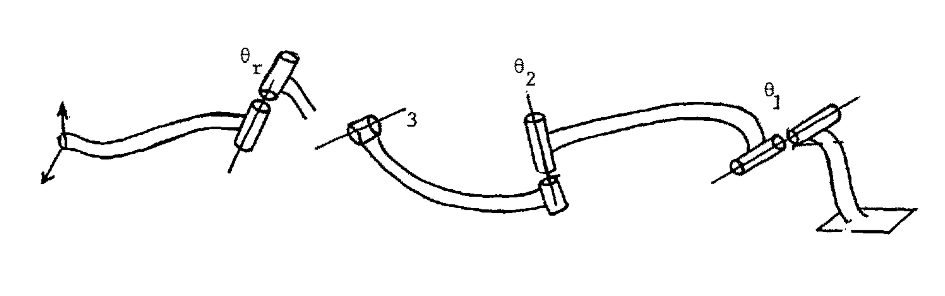
\includegraphics[width=.8\columnwidth]{figures/manip.png}
	\caption{An open kinematic chain. Reprinted from \cite{Brockett1990}.}
	\label{fig:manip}
\end{figure}
%
\begin{figure}[tb!]
	\centering
	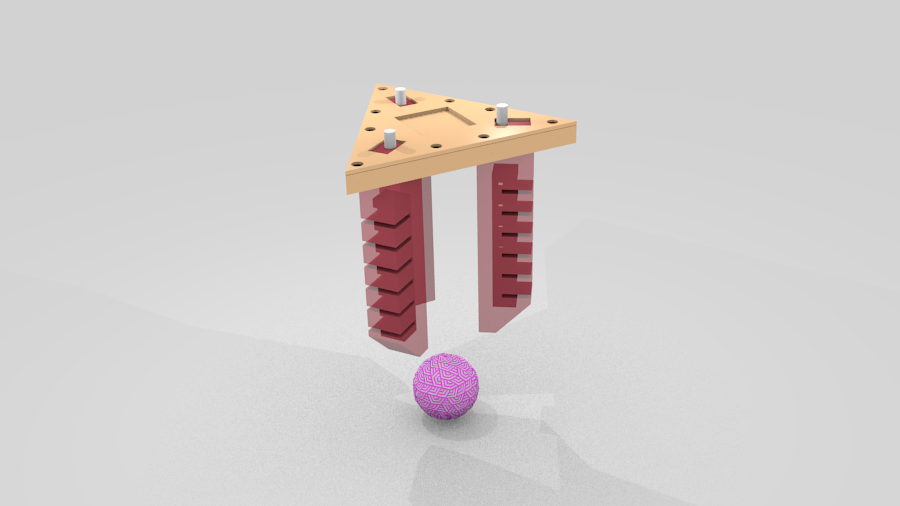
\includegraphics[width=.8\columnwidth]{figures/pneunets.png}
	\caption{The Pneunets Soft Robot}
	\label{fig:pneunets}
\end{figure}
%

\subsection{Screw Axes and  Base Frame}

For consider the kinematic chain of \autoref{fig:manip}. Suppose that we fix a right-handed triad of orthogonal vectors at the tip of each member of the chain, the\textit{ joint space} $Q$ of the robot is the set of all possible values of the joint variables of the robot, which happens to also be the C-space of the robot given that the joint angles completely determine the locations of every link in the robot. 
Similarly, for the soft robot of \autoref{fig:pneunets}, we construct the forward kinematics in a similar fashion; only this time, we do not parameterize the robot links with the joint angles but with the appropriate representation of the deformation of the each pneunet link: an example of a common parameterization approach is to use differential kinematics for arc on the soft robot's body~\cite{Hannan2003}.
%%

For the arm of \autoref{fig:manip}, we may consider that every joint applies a screw motion to all links that protrude from the robot. We take each joint to be displaced by some angle $\theta_i$ so that the end-effector undergoes a displacement of the form $e^{\hat{\xi}_i \theta_i}\homo_i$. The cumulative effect of the robot links on the end-effector is given as (following the notation of \autoref{fig:lienotations}),
%
\begin{align}
\homo_{st}(\theta_1, \ldots, \theta_l) = e^{\hat{\xi}_1 \theta_1}\,e^{\hat{\xi}_2 \theta_2}  \, \ldots e^{\hat{\xi}_l \theta_l} \homo_{st}(0)
\label{eq:fwd_kine}
\end{align}
%
\textit{where $S$ denotes the spatial frame, typically located at the base or shoulder of the robot and $T$ denotes the tool frame, typically situated at the robot's end-effector}. For the system of \eqref{eq:fwd_kine}, we say $\xi_i$ is the twist coordinate of the $i'th$ joint. The equation is the result of moving $\theta_{i+1}$ first before $\theta_i$ while keeping $\theta_i$ fixed. On the other hand, if we reverse the order of the rotations, that would correspond to moving the $i'th$ axis and then rotating the $(i+1)'th$ axis about the new axis, \ie,
%
\begin{align}
	\xi_{i+1}^\prime = \text{Ad}_{e^{\hat{\xi}_i \theta_i}} \xi_{i+1}.
\end{align}
%
We note that the the twist for a revolute joint takes the following form
%
\begin{align}
	\xi_i = \left(\begin{array}{c}
	-\omega \times q_i \\ q_i
	\end{array}\right)
\end{align}
%
where $\omega_i \in \bb{R}3$, is the unit vector in the direction of the twist axis and $q_i \in \bb{R}^3$ is a point along that axis. For a prismatic joint, we have $\xi_i = (v_i, 0)^T$ where $v_i$ is a unit vector along the direction of translation.

\begin{figure}
	\centering
	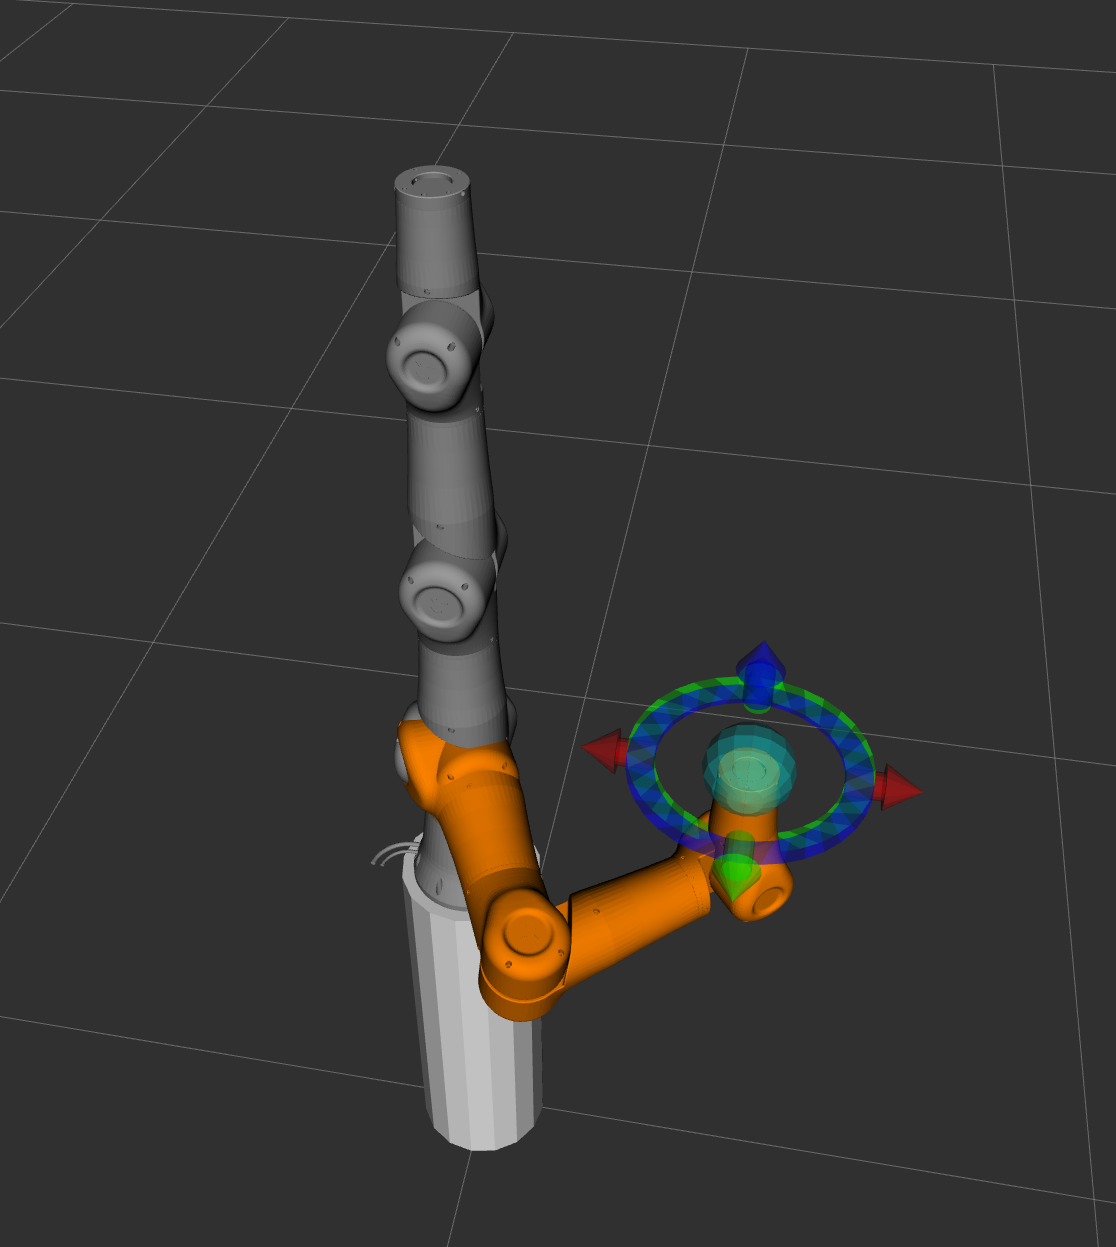
\includegraphics[width=\columnwidth]{figures/torobo7.png}
	\caption{Forward Kinematic Planning for The Torobo 7 Arm}
	\label{fig:torobo7}
\end{figure}
%
\begin{example}
	Consider the Tokyo Robotics (Torobo) arm of \autoref{fig:torobo7}, which is made up of seven joints (six actually, but for now we will assume there is a planar wrist at the end-effector for grasping). The Cartesian coordinates triad are as shown in the orange-colored configuration wherin the blue axis is z, the red axis is $y$-axis and the green axis denotes the $x$-axis. We will take the home position of the robot to be when all joint angles have their angles as $\theta_i = 0$ (this corresponds to the gray pose in the figure). The target pose of the arm is the orange-linked arm shown. The forward kinematics problem would be that given all the six joint angles, and link lengths, find the end-effector pose. We will be leveraging Brockett's product of exponential formula in solving this problem.
	
	For now, suppose the spatial frame is at the base of the robot and the tool frame is on the end-effector. We will for the moment assume that the end-effector is posed at an angle $\theta_7= 0$ as well in the reference frame (colored in gray). The transformation from the base frame to the tool frame is at $\theta = 0$ so that we have from \eqref{eq:fwd_kine}
	%
	\begin{subequations}
		\begin{align}
		&g_{st}(\theta_1,\theta_2,\theta_3,\theta_4,\theta_4, \theta_5, \theta_6, \theta_7) =	e^{\hat{\xi}_1 0}\,e^{\hat{\xi}_2 0},  \, \ldots, e^{\hat{\xi}_l 0} \homo_{st}(0)   \\
		%
		g_{st}(\bm{\theta}) & = g_{st}(0) = \left(\begin{array}{cc}
		\rot(\theta=0) & d \\
		0 & 1
		\end{array} 
		\right) = \left(
		\begin{array}{cc}
		\identity & \left(\begin{array}{c}
		0 
		\\
		%
		0
		\\
		%
		\sum_{i=1}^{i=6} l_i
		\end{array}\right)  \\
		0 & 1
		\end{array} \right).
		\end{align}
	\end{subequations}
\label{ex:torobo7}
\end{example}

\subsection{Screw Axes in Tool Frame}
%
Now, consider again \eqref{eq:fwd_kine}, and recall the properties of the exponential map as given in Def. \autoref{def:exp_map}, we can write 
%
\begin{subequations}
	\begin{align}
	e^{\homo^{-1}P\homo} &= \homo^{-1} e^{P} \homo \\
	\homo \, e^{\homo^{-1}P\homo} &= \homo \, \homo^{-1} e^{P} \homo = e^{P} \homo 
	\end{align}
	\label{eq:mat_exp_reorder}
\end{subequations}
%
Reordering \eqref{eq:fwd_kine} by repeatedly applying \eqref{eq:mat_exp_reorder}, we find that
%
\begin{subequations}
	\begin{align}
	\homo_{st}(\theta_1, \ldots, \theta_l) &= e^{\hat{\xi}_1 \theta_1}\,e^{\hat{\xi}_2 \theta_2}  \, \ldots e^{\hat{\xi}_l \theta_l} \homo_{st}(0) \\
	%
	&= e^{\hat{\xi}_1 \theta_1}\,e^{\hat{\xi}_2 \theta_2}  \, \ldots \homo e^{\homo^{-1} \twistmap_l \homo \theta_l}  \\
	%
	&= e^{\hat{\xi}_1 \theta_1}\,e^{\hat{\xi}_2 \theta_2}  \, \ldots \homo e^{\homo^{-1} \twistmap_{l-1}\homo\theta_{l-1}} e^{\homo^{-1} \twistmap_{l} \homo \theta_l}  \\
	%
	&= e^{\hat{\xi}_1 \theta_1}\,\homo e^{\homo^{-1} \twistmap_{2}\homo\theta_{2}}   \, \ldots e^{\homo^{-1} \twistmap_{l-1}\homo\theta_{l-1}} e^{\homo^{-1} \twistmap_{l} \homo \theta_l}   \\
	%
	&= \homo e^{\homo^{-1} \twistmap_{1}\homo\theta_{1}}  \, e^{\homo^{-1} \twistmap_{2}\homo\theta_{2}}   \, \ldots e^{\homo^{-1} \twistmap_{l-1}\homo\theta_{l-1}} e^{\homo^{-1} \twistmap_{l} \homo \theta_l}  
	\end{align}
	\label{eq:fwd_kine_rev}	
\end{subequations}
%
or 
%
\begin{tcolorbox}[title=Exponential Map in Tool Frame]
	\begin{align}
		\homo_{st}(\theta_1, \ldots, \theta_l) &= \homo e^{\hat{\bodyform}_1\theta_{1}}  \, e^{\hat{\bodyform}_2 \theta_{2}}   \, \ldots e^{\hat{\bodyform}_{l-1} \theta_{l-1}} e^{\hat{\bodyform}_{l} \theta_l} 
	\end{align}
	where $\hat{\bodyform}_i = \homo^{-i} \twistmap_{i}\homo^{i}$ is referred to as the \textbf{body form} of the POE formula. The expression in \eqref{eq:fwd_kine} is notably called the \textbf{space form} of the POE formula.
\end{tcolorbox}

\section{Manipulator parameterization with twists}
%
In the example of \autoref{ex:torobo7}, we can construct the twists for the revolute joints as 
%
\begin{align}
	\omega_1 = \omega_2 = \ldots = \omega_7 = \left(\begin{array}{c}
	0 \\ 0 \\ 1
	\end{array}\right)
\end{align}
%
so that we can choose axis points 
%
\begin{align}
	q_1 &= \left(\begin{array}{c}
	0 \\ 0 \\ l_0
	\end{array}\right) \, 
	%
	q_2 = \left(\begin{array}{c}
	0 \\ 0 \\ l_1
	\end{array}\right) \, 
	%
	q_3 = \left(\begin{array}{c}
	0 \\ 0 \\ l_1 + l_2
	\end{array}\right) \, 
	%
	q_4 = \left(\begin{array}{c}
	0 \\ 0 \\ l_1 + l_2 + l_3
	\end{array}\right) \, 
	%
%	q_4 = \left(\begin{array}{c}
%	0 \\ 0 \\ \sum_{i=1}^{i=4} l_i
%	\end{array}\right) 
	\\
	%	
	q_5 &= \left(\begin{array}{c}
	0 \\ 0 \\  \sum_{i=1}^{i=4} l_i
	\end{array}\right) \, 
	%
	q_6 = \left(\begin{array}{c}
	0 \\ 0 \\  \sum_{i=1}^{i=5} l_i
	\end{array}\right) \, 
	%
	q_7 = \left(\begin{array}{c}
	0 \\ 0 \\  \sum_{i=1}^{i=6} l_i
	\end{array}\right).
\end{align}
%
It follows that we may write the twist as 
%
\begin{subequations}
	\begin{align}
	\xi_1 &= \left(\begin{array}{c}
	0 \\ 0 \\ 0 \\ 0\\ 0 \\ 0 
	\end{array}\right) \, 
	%
	\xi_2 = \left(\begin{array}{c}
	0 \\ 0 \\ 0 \\ 0\\ 0 \\ l_1
	\end{array}\right) \, 
	%
	\xi_3 = \left(\begin{array}{c}
	0 \\ 0 \\ 0 \\ 0 \\ 0 \\ l_1 + l_2
	\end{array}\right) \, 
	%
	\xi_4 = \left(\begin{array}{c}
	0 \\ 0 \\0 \\ 0 \\  l_1 + l_2 + l_3
	\end{array}\right) \, \\
	%\end{align}
	%%
	%\begin{align}
	\xi_5 &= \left(\begin{array}{c}
	0 \\ 0 \\ 0 \\ 0 \\ 0 \\ \sum_{i=1}^{i=4} l_i
	\end{array}\right) \, 
	%
	\xi_6 = \left(\begin{array}{c}
	0 \\ 0 \\  0 \\ 0 \\ 0 \\ \sum_{i=1}^{i=5} l_i
	\end{array}\right) \, 
	%
	\xi_7 = \left(\begin{array}{c}
	0 \\ 0 \\   0 \\ 0 \\ 0 \\ \sum_{i=1}^{i=6} l_i
	\end{array}\right)
	\end{align}
\end{subequations}
%
where the screw axes in the base frame are as given in \autoref{tab:torobo_screw_space_form}
%
\begin{table}[tbph!]
	\caption{Table of Screw Axes for the Torobo Arm.}
	\centering
	\begin{tabular}{|c|c|c|| c|c|c|}
		\hline \rule[-2ex]{0pt}{5.5ex}  
		$i$ & $\omega_i$ & $v_i$ & $i$ & $\omega_i$ & $v_i$\\
		\hline \rule[-2ex]{0pt}{5.5ex}  
		1  & (0, 0, 0) & (0, 0, 0) & 4  & (0, 0, $l_1+l_2+l_3$) & (0, 0, 0) \\	
		\hline \rule[-2ex]{0pt}{5.5ex}  
		2  & (0, 0, $l_1$) & (0, 0, 0) & 5  & (0, 0, $l_1+l_2+l_3+l_4$) & (0, 0, 0)  \\
		\hline \rule[-2ex]{0pt}{5.5ex}  
		3  & (0, 0, $l_1+l_2$) & (0, 0, 0) & 6  & (0, 0, $l_1+l_2+l_3+l_4+l_5$) & (0, 0, 0)  \\
		\hline \rule[-2ex]{0pt}{5.5ex}  
		7  & (0, 0, $l_1+l_2+l_3+l_4+l_5+l_6$) & (0, 0, 0)  & 7  & (0, 0, $l_1+l_2+l_3+l_4+l_5+l_6$) & (0, 0, 0) \\
		\hline
	\end{tabular}
\label{tab:torobo_screw_space_form}
\end{table}
%
We may now write the various exponents as 
%
\begin{subequations}
	\begin{align} 
	e^{\hat{\xi}_1 \theta_1} &= \left(\begin{array}{cccc}
	\cos \theta_1 & -\sin \theta_1 & 0 & 0 \\
	\sin \theta_1 & \cos \theta_1 & 0 & 0 \\
	0 & 0 & 1 & 0 \\
	0 & 0 & 0 & 1
	\end{array}\right), \quad
	%	
	e^{\hat{\xi}_2 \theta_2} = \left(\begin{array}{cccc}
	\cos \theta_2 & -\sin \theta_2 & 0 & l_1 \sin\theta_2 \\
	\sin \theta_2 & \cos \theta_2 & 0 & l_1 (1-\cos \theta_2) \\
	0 & 0 & 1 & 0 \\
	0 & 0 & 0 & 1
	\end{array}\right) \\
	%
	e^{\hat{\xi}_3 \theta_3} &= \left(\begin{array}{cccc}
	\cos \theta_3 & -\sin \theta_3 & 0 & (l_1 + l_2)\sin\theta_3  \\
	\sin \theta_3 & \cos \theta_3 & 0 & (l_1 + l_2) (1-\cos \theta_3)\\
	0 & 0 & 1 & 0 \\
	0 & 0 & 0 & 1
	\end{array}\right), \quad
	%	
	\nonumber \\
	& \ldots \quad \ldots\quad \ldots\quad \ldots
	\nonumber \\
	%
	e^{\hat{\xi}_7 \theta_7} &= \left(\begin{array}{cccc}
	1 & 0 & 0 & 0 \\
	0 & 1 & 0 & 0 \\
	0 & 0 & 1 & \theta_7 \\
	0 & 0 & 0 & 1
	\end{array}\right)
	\end{align}  
\end{subequations}
%
whereupon we find that the rotation and translation are 
%
\begin{align}
	R(\theta) = \left(\begin{array}{ccc}
	\cos(\theta_1+\ldots + \theta_7) & \sin(\theta_1+\ldots + \theta_7) &0 \\
	\sin(\theta_1+\ldots + \theta_7) & \cos(\theta_1+\ldots + \theta_7) &0 \\
	0 & 0 & 1
	\end{array}\right), 
	\nonumber \\
	d(\theta) = \left(\begin{array}{c}
	-l_1 \sin(\theta_1) - l_2 \sin(\theta_1+ \theta_2) \ldots - l_7\sin(\theta_1+  \ldots + \theta_7) \\
	%
	l_1 \cos(\theta_1) + l_2 \cos(\theta_1+ \theta_2) \ldots - l_7\cos(\theta_1 + \ldots + \theta_7) \\
	%
	l_0  \theta_7
	\end{array}\right) 
\end{align}

\begin{homework}
	Now consider the orange robot configuration of \autoref{fig:torobo7}. Suppose that the joint angles from the base out to the tool frame is given as $\{0, 0, -90, 90, 0, 0, 0\}$ . Determine the position and orientation of the end effector. 
\end{homework}

\section{The Universal Robot Description Format}
%
When we program robots, it is often helpful to write the transformation from one frame to another in a very modular file format. Typically for industrial arms, there are multiple frames that enable the software engineer to effectively carry out transformations. Hardcoding these transformations as we see in the Torobo example is an exercise in tediousness. Thankfully, the Open Robotics Foundation maintains the \textit{Robot Operating System}, popularly referred to as ROS, which allows us to describe the interrelationship among the various links and joints of the robot to the end that transformation is simplified for the user. This file format is referred to as \textit{Universal Robot Description Format}. They let the computer understand the nature of the robot. 

Note that the URDF format provided by Open Robotics is only valid for open kinematic chains and wheeled robots. The engine used in writing the ROS and gazebo frameworks are not optimized for parallel manipulators and soft materials as yet. In addition, Gazebo, uses a pseudo-URDF file called \textsc{SDF}. 

\begin{homework}
	For this homework, you are asked to get familiar with the URDF Tutorials \href{http://wiki.ros.org/urdf}{here}: http://wiki.ros.org/urdf. In particular, go through the PR2 composition in the tutorial given. The knowledge gained from this tutorial will be helpful as we go forward in this class.
\end{homework}

\section{Velocity Kinematics}

Suppose we represent the set of all joint angles of an open kinematic chain robot arm as $\bm{\theta} = \{\theta_1 \times \theta_2 \ldots \theta_l\} \in \ren$. Suppose further that the velocity of the end-effector is governed by the following first-order differential equation:
%
\begin{align}
	\homo(t) = \homo_{st}(\bm{\theta}(t)), \, \bm{\theta} \in \ren.
\end{align}
%
It follows that the end-effector velocity is 
%
\begin{align}
	\dot{\homo}(t) = \sum_{i=1}^{n} \dfrac{\partial \homo_{st}(\bm{\theta})}{\partial \theta_i} \dfrac{d \theta_i(t)}{d t} =  \sum_{i=1}^{n} \dfrac{\partial \homo_{st}(\bm{\theta})}{\partial \theta_i} \dot{\theta}_i, \quad i = 1, \ldots, n
	\label{eq:jacob_gen}
\end{align}
%
or written more succinctly,
%
\[
	\dot{\homo}(t) = \jacob_{st}(\bm{\theta})\dot{\bm{\theta}}
\]
%
where $\jacob(\theta) \in \bb{R}^{n\times n}$ is referred to as the \textbf{Jacobian}. We see from the structure of the derived Jacobian that the Jacobian is only naturally expressed when the forward map of the robot is of the form $\homo: \ren \rightarrow \bb{R}^p$ so that the derivative of the map with respect to the joint angles is naturally meaningful. Not so when we have the forward map as $g: \ren \rightarrow SE(3)$. Here, the Jacobian would not naturally expressible  since $\homo$ is a matrix-valued function. You start seeing why screw theory helps simplify the geometry of robotics. If we were to choose a local coordinates in the Lie Group $SE(3)$, the description would only be valid locally so that the natural geometric structure of the rigid body motion would be eliminated.

\section{Singularities in Rigid Bodies and The Manipulability Ellipsoid}
%
For consider the two link planar arm of \autoref{fig:planar_rot}.  We illustrate the geometry of that planar arm more clearly in \autoref{fig:planar_manip} whose forward kinematics is
%
\begin{figure}[tb!]
	\centering
	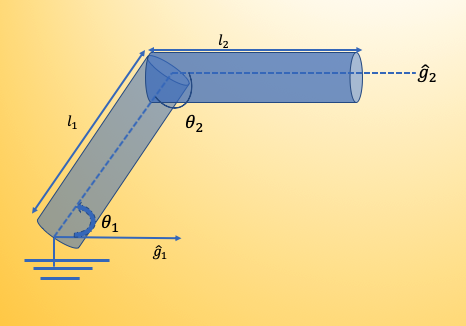
\includegraphics[width=.7\columnwidth]{figures/planar_manip.png}
	\caption{An illustration of the geometric configuration of the planar arm}
	\label{fig:planar_manip}
\end{figure}
%
\begin{subequations}
	\begin{align}
	\homo_1 = l_1 \cos \theta_1 + l_2 \nonumber \\
	%
	\homo_2 = l_1 \sin \theta_1 + l_2 \sin(\theta_1+\theta_2)
	\end{align}
\end{subequations}
% 
and whose first order time derivative yields,
%
\begin{subequations}
	\begin{align}
	\dot{\homo}_1 = -l_1 \dot{\theta}_1 \sin \theta_1  \nonumber \\
	%
	\dot{\homo}_2 = l_1 \dot{\theta}_1 \cos \theta_1 + l_2 (\dot{\theta}_1+\dot{\theta}_2) \cos(\theta_1+\theta_2).
	\end{align}
\end{subequations}
%
Vectorizing, we have
%
\begin{align}
	\left(\begin{array}{c}
		\dot{\homo}_1 \\
		%
		\dot{\homo}_2
	\end{array}\right) = \left(\begin{array}{cc}
	-l_1  \sin \theta_1 & 0 \\
	%
	 l_1  \cos \theta_1 + l_2  \cos(\theta_1+\theta_2) &  l_2 \dot{\theta}_2 \cos(\theta_1+\theta_2)
	\end{array}\right)
	%
	\left(\begin{array}{c}
	\dot{\theta}_1 \\
	%
	\dot{\theta}_2
	\end{array}\right)
\end{align}
% 
so that the velocity of the tip point of the 2R robot arm can be written as 
%
\begin{align}
	v_{tip} = J_1(\theta)\dot{\theta}_1 + J_2(\theta)\dot{\theta}_2.
\end{align}
%
We can always guarantee a tip point velocity as long as the columns of the manipulator Jacobian are not collinear. When collinearity occurs, the robot ends up in a \textit{singular configuration} and the Jacobian loses rank (more on this later on). Formally, we say a manipulator is in a singular configuration when the tip of the robot is unable to move arbitrarily in specific directions.

\subsection{The Manipulability Ellipsoid}
%
We now formally introduce the manipulability ellipsoid of the robot arm. When you start designing robot mechanisms, you would need to understand how arbitrarily changing the position and orientation of the end-effector at the tip of the robot arm is a function of the joint velocities and their positions. 
\begin{definition}
	The quantitative index that defines the set of all end-effector velocities that are realizable by joint velocities under a magnitude constraint (\eg a Euclidean norm  $<=1$) such that \textit{those end-effector velocities are \textbf{large and spherical} as much as possible} is the \textbf{manipulability measure} of the robot.
\end{definition}

The manipulability measures the performance of the arm's kinematics (motions) in order for us to optimize the size of the robot. To illustrate the intuitive mesaning of the manipulability measure, play with the cdf file located on the wolfram cloud at this \href{https://demonstrations.wolfram.com/ManipulabilityEllipsoidOfARobotArm/}{web address}. What happens, when you set all the angles of the robot to zero or $180^\circ$? Notice that the manipulability becomes $0$. Coincidentally, we find that this is a situation that occurs when the robot is at a singularity and the manipulability ellipsoid is at its lowest coverage within the manipulator workspace.

\begin{homework}
	Explain what happens when you adjust the parameters of the robot as follows 
	%
	\begin{itemize}
		\item Keep $\theta_1 = \theta_3 = 0$ and vary $\theta_2$. What do you notice about the size of the ellipsoid? How does it affect the mannipulability measure? 
		%
		\item Keep $\theta_2 = \theta_3 = 0$ and set $\theta_1$ at $\pi/2$. What happens to the shape of the ellipsoid? Report the manipulability measure.
		%
		\item Keep any  two the joints at $180^\circ$ and make the other joint $0^\circ$. What do you notice?
	\end{itemize}
\end{homework}

From the \href{http://scriptedonachip.com/downloads/Videos/manipulability.mp4}{video} of the ellipsoids, we notice that the closer the ellipsoids are in area to a circle, the more the freedom we obtain in being able to move the tip in arbitrary directions.  So we define the \textit{manipulability measure} as 
%
\begin{align}
	\sqrt{\dot{q}_1^2(t)+\dot{q}_2^2(t)+\ldots + \dot{q}_l^2(t)} \le 1
\end{align}
%
which is to say the the bound on the Euclidean norm of all joint angle velocities such that it is less than unity and we define the manipulability ellipsoid as 
%
\begin{align}
	\{ v(t) J^{-T} \cdot J^{-1} \cdot v(t) \le 1, v(t): Rank(J) \}
 \end{align}

\section{The Manipulator Jacobian}

Here, we are concerned with the magnitudes of the joint velocities when the  $\dot{\theta}_i = 1$ and all other joint velocities are $0$. This determines the twist, which we treated in \autoref{chap:rbm}. Particularly, we separate the treatments of the spatial manipulator Jacobian (\ie the the Jacobian where each column of $J$ is a screw axes in the base or a fixed spatial frame, $s$) and the body manipulator Jacobian (\ie the Jacobian where each column of $J$ is a screw axes in the the end-effector frame, $b$).

\subsection{Spatial Jacobian}
%
Consider the general Jacobian of \eqref{eq:jacob_gen}, suppose now that $g_{st} \rightarrow SE(3)$ is a forward kinematic map for the manipulator and the joints traverse a path $\theta(t) \in Q$, so that the end-effector follows a path $\homo_{st}(\theta(t)) \in SE(3)$. The instanteneous spatial velocity of the end-effector would be the set 
%
\begin{align}
	\hat{\eta}^s_{st} = \dot{\homo}_{st}(\theta) \homost^{-1}(\theta)
	\label{eq:spatial_jacob}
\end{align}
%
Applying the chain rule as before (\cf \eqref{eq:jacob_gen}), we have 
%
\begin{align}
	\hat{\eta}^s_{st}  = \sum_{i=1}^{n} \left(\dfrac{\partial \homo_{st}({\theta})}{\partial \theta_i} \dot{\theta}_i \right) \homost^{-1}(\theta) =  \sum_{i=1}^{n} \left( \dfrac{\partial \homo_{st}({\theta})}{\partial \theta_i} \homost^{-1}(\theta) \right) \dot{\theta}_i.
\end{align}
%
In twist coordinates, we write the above as 
%
\begin{align}
		\hat{\eta}^s_{st}  = J_{st}^s(\theta) \dot(\theta)
\end{align}
%
where
%
\[
	J_{st}^s = \left[\left(\dfrac{\partial \homo_{st}({\theta})}{\partial \theta_1} \homost^{-1}\right)^\vee 
							\ldots
						    \left(\dfrac{\partial \homo_{st}({\theta})}{\partial \theta_l} \homost^{-1}\right)^\vee 
							\right]
\]
%
and the $i'th$ joint twist transformed by $e^{\twistmap_1 \theta_1} \ldots e^{\twistmap_{i-1}\theta_{i-1}}$ from the $i'th$ joint in the reference configuration to the current configuration of the manipulator is
%
\[
	\left(\dfrac{\partial \homo_{st}({\theta})}{\partial \theta_1} \homost^{-1}\right)^\vee = \text{Ad}_{\left(e^{\twistmap_1 \theta_1}\ldots e^{\twistmap_{l-1} \theta_{l-1}}\right)}\twistmap_l :\equiv \twistcoord^\prime.
\]
%
It therefore follows that 
%
\begin{align}
	J_{st}^s(\theta) = \left[\twistcoord_1, \twistcoord_2^\prime  \ldots \twistcoord^\prime_l \right]
\end{align}
%
We thus see that the \textit{i'th column of the Jacobian corresponds to the i'th joint twist, transformed to the current manipulator configuration.}

\subsection{The Body Jacobian}
%
In body coordinates, we rewrite \eqref{eq:spatial_jacob} as 
%
\begin{align}
\hat{\eta}^b_{st} = J^b_{st}(\theta)\dot{\theta}
\label{eq:body_jacob}
\end{align}
%
so that 
%
\begin{subequations}
	\begin{align}
	J_{st}^b(\theta) =  \left[\twistcoord_1^\star, \twistcoord_2^\star  \ldots \twistcoord^\star_{l-1} \twistcoord^\star_{l} \right] \\
	%
	\twistcoord_i^\star = \text{Ad}^{-1}_{\left(e^{\twistmap_1 \theta_1}\ldots e^{\twistmap_{l} \theta_{l}}\homost(0)\right)}\twistmap_i
	\end{align}
\end{subequations}
%
where the $\homost(0)$ term allows us the freedom to choose the base frame in order to simplify our calculations (\eg choose $\homost(0) = I$.

Before we close this section, we note the following relations between the two Jacobians:
%
\begin{align}
	J_{st}^s(\theta) = Ad_{\homost(\theta}J_{st}^b(\theta).
\end{align}
%
These spatial and body manipulator Jacobians are useful in finding the instanteneous velocity of the tip point in the end-effector frame. Suppose we let $q^b$ be this tip point in body coordinates, we can find the velocity $v^b$ in the tool frame (body coordinates) as 
%
\begin{align}
	v^b_q = \hat{\eta}_{st}^b q^b = \left(J_{st}^b(\theta) \dot{\theta}\right)^\wedge q^b.
\end{align}
%
The logic above applies in spatial coordinates (\ie the base frame), whereupon we have
%
\begin{align}
v^s_q = \hat{\eta}_{st}^s q^s = \left(J_{st}^s(\theta) \dot{\theta}\right)^\wedge q^s
\end{align}

Notice from \eqref{eq:spatial_jacob} that 
%
\begin{align}
	\dot{\theta}(t) = \left(J_{st}^s(\theta)^{-1} \eta_{st}^s (t) \right)
\end{align}
%
implying that we do not need the inverse kinematics of the manipulator of the robot if we want to move an arm from one end-effector pose to another since we know the relationship between the joint velocities and the end-effector velocity.

\begin{homework}
	Explain how you would go about implementing the last part of the above statement for the planar robot arm of \autoref{fig:planar_manip}.
\end{homework}

\section{Inverse kinematics}
%
We formally define the inverse kinematics problem as follows: given a desired configuration for the end-effector, $\homo_d$, find the joint angles necessary for achieving that configuration. Mathematically, we can think of this as being given a forward kinematic map $\homost: Q \rightarrow SE(3)$, and $\homo_d$, find the desired joint angles by solving 
%
\begin{align}
	\homost(\theta) = \homo_d
\end{align}
%
for some $\theta \in Q$. It is noteworthy to here point out that the IK problem mat have multiple solutions,, a unique solution or no solution at all. It is typical to use numerical optimization approaches to solve these problems in practice. In ROS, there are different IK libraries that are available such as the ones from \textsc{KDL} or 

\begin{example}
	Consider the two-link planar arm of \autoref{fig:ik_ex}. This example is taken from \cite{MurrayBook}. We know the forward kinematics to be 
	%
	\begin{align}
		x = l_1 \cos \theta_1 + l_2 \cos(\theta_1 + \theta_2) \nonumber \\
		%
		y = l_1 \sin \theta_1 + l_2 \sin(\theta_1 + \theta_2).
	\end{align}
	%
	In order to solve for $\theta_1$ and $\theta_2$ given $x$ and $y$, we use polar coordinates to parameterize the geometry (see the right inset). We see that 
	%
	\begin{subequations}
		\begin{align}
			r &= \sqrt{x^2 + y^2} \\
			\theta_2 &= \pi \pm \alpha \\
			\alpha &= \cos^{-1} \frac{l_1^2 + l_2^2- r^2}{2 l_1 l_2}.
		\end{align}
	\end{subequations}
	%
	That is, $\theta_2$ could take on two possible values when $\alpha \neq 0$. The second value of $\theta_2$ is shown by the dashed line, called the ``flipped' solution''. We find $\theta_1$ by solving
	%
	\begin{align}
	\theta_1 = a\tan2(y,x) \pm \beta, \quad \beta = \cos^{-1}\left(\frac{r^2 + l_1^2 - l_2^2}{2 l_1l_2}\right)
	\end{align}
	%
	with the condition that the sign of $\alpha$ must correspond to the one used for $\beta$.
	%
\end{example}


\begin{figure}[tb!]
	\centering
	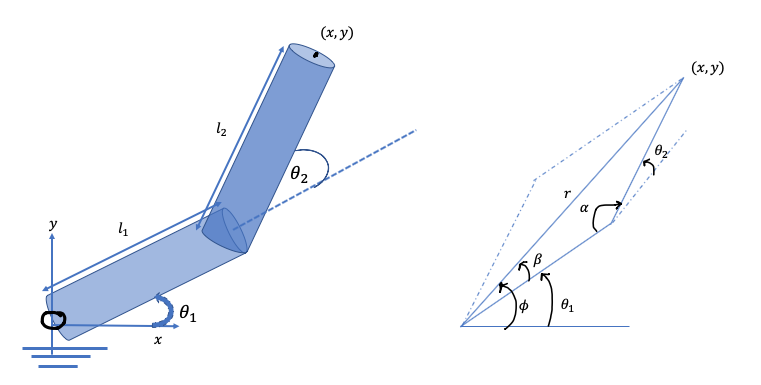
\includegraphics[width=.8\columnwidth]{figures/ik_ex.png}
	\caption{Inverse Kinematics of a two-link planar manipulator}
	\label{fig:ik_ex}
\end{figure}
%\chapter{Statics and Velocity Kinematics}
\label{chap:statics}

\section{Singularities in Configurations}

\section{The antisymmetric matrix}

\section{Derivation of Rotation Matrices}

\section{The Manipulator Jacobian: Derivation}

\section{Relating the Spatial to Body Jacobian}

\section{Velocities of the tip and tool frames}

\section{Decoupling singularities}

\section{The principle of virtual work}

\section{Manipulability}
%\chapter{Robot Dynamics and Control}
%
At issue in this chapter are the motions of various components of a robot given the forces, torques and momentum that act upon it. In rigid body dynamics, we typically represent these dynamics using nonlinear, second-order differential equations which are a function of the kinematics and kinetics of the robot.  While in principle, we can individually sum the forces and torques acting on an object, in practice, it is easier working with the system's \textit{Lagrangian, a summation of all the mechanical energies of the system}, as this tends to be less prone to error than summing together the Coriolis, centrifugal and inertial forces acting on the robot's links. 

The control problem for robot manipulators requires us knowing the dynamics of the robot. This is sometimes called the \textit{inverse dynamics problem} of a robot manipulator, \ie given the mass matrix, Coriolis forces and torques for all the individual robot joints, find the control law that yields a desired motion in space. Assuming that the model we have found is perfect, the control law is very simple. In practice, a feedback control (and sometimes coupled with a robust control) law needs to be derived to correct unmodeled uncertainties and improve trajectory following~\cite{Ogunmolu18IROS}.

There are two methods of controlling a rigid robot: \textit{joint space control} and \textit{workspace control}. In joint space control, a manipulation or navigation task is converted to a desired trajectory for the joints of a robot. We then find a control law to apply actuator torques to the joints of the robot in order to follow a given trajectory. In workspace control, the dynamics and control problem is changed into the task space of the robot so that trajectory commands are given in the coordinates of the end-effector.

\section{Lagrangian for Mechanical Systems }
%
For a system of $n$ particles obeying Newton's second law of motion, the time rate of change of the particle's momentum is the external force applied on the particle. Suppose $F_i$ is the applied force on the $i^{th}$ particle, $m_i$ is the particle's mass, and $r_i$ is the position, it follows from Newton's law that 
%
\begin{align}
	F_i = m_i r_i \quad r_i \in \bb{R}^3, i = 1, \ldots, n.
	\label{eq:RBD_Newton}
\end{align}
%
We are interested in the material description of the body where the overall degrees of freedom is constrained by the coupling between the individual robots. In the \textit{material description}, we are interested with the body-points as it is treated in analytical dynamics, where it is typical to work with first, second, $\ldots$, $n^{th}$ masses. As such, we write out the constraints which govern the particle's positions as the following holonomic constraint\footnote{
%
If time enters the relation in the equation explicitly, then we have a rheonomic constraint, otherwise, the constraint is called sclerenomic constraint. A particle suspended from a tight rope in 3D space would be an example of a rheonomic constraint with the equation, $(x_1-1)^2  + (x_2 - b)^2 + (x_3-c)^2 - r^2 = 0$, while a particle on a carousel would be a sclerenomically-constrained system. Such a system would be described by the following equation, $x_1 = a \cos(\omega t + \phi); x_2 = a \sin (\omega t + \phi).$}. These are the constraints of position in a system.  
%
\begin{align}
g_i(r_1, \ldots, r_n) = 0, \quad j = 1, \ldots, k.
\label{eq:holonomic}
\end{align} 
%
In general, holonomic constraints are systems whose \dofs can be written in an algebraic relationship where the positions are a direct function of velocities. 

Constraints act on a system of particles through the application of \textit{constraint forces} such that they are forces that are normal to smooth surfaces in $\bb{R}^n$. Suppose we have the basis for the constraint forces (not necessarily orthonormal) as $\Gamma_1, \ldots, \Gamma_k \in \bb{R}^3n$ and $\lambda_j$ are the respective scaling factors for the $j^{th}$ basis elements, then we can write Newton's second law that governs the system of equations as 
%
\begin{align}
	F = \begin{bmatrix}
	m_1 \, I &  & 0 \\
	%
	& \ddots & \\
	%
	0 & & m_n \, I
	\end{bmatrix}
	%
	\begin{bmatrix}
	\ddot{r}_1  \\ \vdots \\ \ddot{r}_n
	\end{bmatrix} +  \sum_{j=1}^{k} \Gamma_j \lambda_j
\end{align}
%
where $\Gamma_j$ for the holonomic constraints of \eqref{eq:holonomic} can be taken as the gradients of $g_j$, essentially the level sets of $g_j(r) = 0$. 
%
While simple, this approach does not scale well to the configuration of the sort of rigid bodies we deal with in robotics. A better approach is to use a smaller set of variables that parameterizes the configuration of the system. For a system of $n$ particles with $k$ constraints, we find a set of $m = 3n -k$ variables $q_1, \ldots , q_m$ and smooth functions $f_1, \ldots, f_n$ such that 
%
\begin{align}
	r_i = f_i(q_1, \ldots, q_m), \quad i = 1, \ldots, n \\
	%
	g_j(r_1, \ldots, r_n) = 0, \quad j = 1, \ldots, k
\end{align}
%
where $q_i$'s are the generalized coordinates of the system, which in the case of robot manipulators is almost always the joint angles.  The forces expressed along the coordinates of the generalized coordinates of position are referred to as \textit{generalized forces}. 

\section{Euler-Lagrange Equations}
%
For a kinetic energy $T$ and a potential energy $V$, the \textit{Lagrangian, $L$}, of the system in generalized coordinates is the difference between the kinetic and potential energy, \ie
%
\begin{align}
L(q, \dot{q}) = T(q, \dot{q}) - V(q).
\label{eq:lagrange}
\end{align}
%
In general, we write the kinetic energy in the form, 
%
\begin{align}
	T(\theta) = \frac{1}{2} \sum_{i = 1}^{n} \sum_{j = 1}^{n}  m_{ij}(\theta) \dot{\theta}_i \dot{\theta}_j = \frac{1}{2} \dot{\theta}^T M(\theta) \dot{\theta}
\end{align}
% 
with $m_{ij}$ being the ($i, j$)th element of the mass matrix $M(\theta)$. 
%
The equations of motion for a rigid body articulated system is of the form
%
\begin{align}
\dfrac{d}{dt}\dfrac{\partial L}{\partial \dot{q}_i} - \dfrac{\partial L}{\partial q_i} = \torque_i, \quad i = 1, \ldots, m
\label{eq:lagrange_compo}
\end{align}
%
where $\torque_i$ is the torque acting on the $i^{th}$ generalized coordinate. Hence, we can explicitly write the dynamics as 
%
\begin{align}
\sum_{j=1}^{n} m_{ij}(\theta) \ddot{\theta}_j + \sum_{j = 1}^{n} \sum_{k = 1}^{n} \Gamma_{ijk}(\theta) \dot{\theta}_j \dot{\theta}_k + \dfrac{\partial V}{\partial \theta_i } = 	\torque_i, \quad i = 1, \ldots, n
\end{align} 
%
with $\Gamma_{ijk}(\theta) $ being the so-called \textbf{Christoffel symbols of the first kind}, defined as, 
%
\begin{align}
	\Gamma_{ijk}(\theta)  = \frac{1}{2}\left(\dfrac{\partial m_{ij}}{\partial \theta_k} + \dfrac{\partial m_{ik}}{\partial \theta_k} - \dfrac{\partial m_{jk}}{\partial \theta_i}.
	\right)
\end{align}
%
Essentially, the Christoffel symbols determine the Coriolis and centripetal terms in the matrix $\coriolis(\theta, \dot{\theta}$ as we shall see shortly and they are by-products of the mass matrix $\massinertia(\theta)$. 
%
Written in matrix form equation, we can write the Euler-Lagrange equation of \eqref{eq:lagrange_compo} as
%
\begin{align}
\dfrac{d}{dt}\dfrac{\partial L}{\partial \dot{q}} - \dfrac{\partial L}{\partial q} = \torque.
\label{eq:lagrange_deri}
\end{align}
%
Equation \eqref{eq:lagrange_deri} is elegant because it reduces the number of coordinates we need to work with from $n$ to $m$ (the number of generalized coordinates) for a system. It can be rewritten as 
% 
\begin{align}
M(\theta) \ddot{\theta} + C(\theta, \dot{\theta}) + N(\theta) = \torque,
\label{eq:lagrange_mat}
\end{align}
%
where we see that the Coriolis and centripetal terms enter the torque equation as quadratic factors for the velocity terms, \ie
%
\begin{align}
	M(\theta) \ddot{\theta} + \dot{\theta}^T \Gamma(\theta) \dot{\theta} + N(\theta) = \torque
\end{align}
%
with $\Gamma_i(\theta)$ being an $n\times n$ matrix with the $(j,k)$the entry as $\Gamma_{ijk}$ and the Coriolis matrix has the $(j,k)$ entry as 
%
\begin{align}
	C_{ij}(\theta, \dot{\theta}) = \sum_{k=1}^{n} \Gamma_{ijk}(\theta) \dot{\theta}_k.
\end{align}
%
Thus for a given robotic mechanical system, finding the dynamics is tantamount to deriving the kinetic and potential energies for the system based on that particular system characteristics. In the next two subsections, we will treat two examples -- a simple pendulum system and the dynamics of a mecanum wheel robot. 

\section{Dynamics of a spherical Pendulum}
%
We now consider the double pendulum of \autoref{fig:double-pendulum} with masses $m_1$ and $m_2$. We would like to find the overall torque of the system based on the Euler-Lagrange system of equations we just derived.
%
\begin{figure}[tb!]
	\centering
	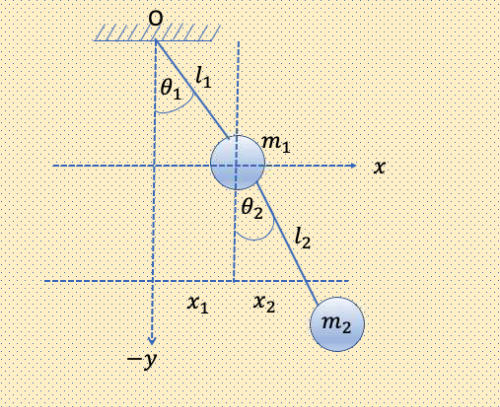
\includegraphics[width=.8\columnwidth]{figures/double-pendulum.png}
	\caption{The double pendulum with configuration is decribed by the angles $\theta_1$ and $\theta_2$.}
	\label{fig:double-pendulum}
\end{figure}
%
First, we write out the position vector of the masses as follows,
%
\begin{align}
	r(\theta_1, \theta_2) = \left(\begin{array}{c|c}
	l_1 \sin \theta_1 & l_1 \sin \theta_1  + l_2 \sin \theta_2
	\\
	-l_1 \cos \theta_1 & -l_1 \cos \theta_1  - l_2 \cos \theta_2
	\end{array}\right)
\end{align}
%
whose time derivative and second time derivative are respectively
%
\begin{align}
	\dot{r} = \left(\begin{array}{c|c}
	\dot{\theta}_1 l_1 \cos \theta_1 & \dot{\theta}_1 l_1 \cos \theta_1  + \dot{\theta}_2 l_2 \cos \theta_2
	\\
	\dot{\theta}_1 l_1 \sin \theta_1 & \dot{\theta}_1 l_1 \sin \theta_1  + \dot{\theta}_2 l_2 \sin \theta_2
	\end{array}\right)
\end{align}
%
and
%
\begin{align}
\ddot{r} = \left(\begin{array}{c|c}
\ddot{\theta}_1 l_1 \cos \theta_1 - \dot{\theta}_1^2 l_1 \sin \theta  & \ddot{\theta}_1 l_1 \cos \theta_1 - \dot{\theta}_1^2 l_1 \sin \theta  + \ddot{\theta}_2 l_2 \cos \theta_1 - \dot{\theta}_2^2 l_2 \sin \theta
\\
\ddot{\theta} l_1  \sin \theta_2 + \dot{\theta}_1^2 l_1 \cos \theta_1  & 
\dot{\theta}_1^2 l_1 \cos \theta_1  + \dot{\theta}_2^2 l_2 \cos \theta_2  + \ddot{\theta}l_1 \sin \theta_1 + \ddot{\theta}_2 l_2 \sin \theta_2 
\end{array}\right)
\end{align}
%
with the associated co-kinetic~\cite{Stramigioli2001} and potential energies
%
\begin{align}
	T = \frac{1}{2} m \|\dot{r}\|^2 = \frac{m_1}{2}l_1^2 \dot{\theta}_1^2 + \frac{m_2}{2}\left(l_1^2 \dot{\theta}_1^2 + l_2^2 \dot{\theta}_2^2 + 2 l_1 l_2 \dot{\theta}_1 \dot{\theta}_2 \cos(\theta_1 - \theta_2) \right)
\end{align}
%
and
%
\begin{align}
	V = g(m_1 \, y_1 + m_2\, y_2) = -m_1gl_1 \cos \theta_1 - m_2 g \left(l_1 \cos \theta_1 + l_2 \cos \theta_2\right)
\end{align}
%
where $g$ in this case denotes the gravitational acceleration.
%
We thus have the Lagrangian of the system as 
%
\begin{align}
	L & = T - V \nonumber \\
	  & = \frac{1}{2}(m_1 + m_2)l_1^2 \dot{\theta}_1^2 + \frac{1}{2}m_2 l_2^2 \dot{\theta}_2^2 + m_2l_1 l_2 \dot{\theta}_1 \dot{\theta}_2 \cos(\theta_1 - \theta_2) + (m_1 + m_2) g l_1 \cos \theta_1 + m_2 g l_2 \cos \theta_2 
\end{align}
%
Now writing the derivatives of the canonical momenta, we have
%
\begin{align}
\dfrac{\partial L}{\partial \dot{r}} &=  (m_1+m_2)l_1^2 \dot{\theta}_1 + m_2 l_2^2 \dot{\theta}_2 + m_2 l_1 l_2 \dot{\theta}_2 \cos(\theta_1 - \theta_2) + m_2 l_1 l_2 (\dot{\theta}_1 + \dot{\theta}_2 )  \cos(\theta_1 - \theta_2) 
% (\dot{\theta}_1 + \dot{\theta}_2) 
\end{align}
%
whereupon, 
%
\begin{align}
	\dfrac{d}{dt}\dfrac{\partial L}{\partial \dot{r}} &=  (m_1+m_2)l_1^2 \ddot{\theta}_1 + m_2 l_1 l_2 \ddot{\theta}_2 \cos(\theta_1 - \theta_2) -  m_2 l_1 l_2 \dot{\theta}_2 \sin(\theta_1 - \theta_2) (\dot{\theta}_1 - \dot{\theta}_2) \nonumber \\
	& \quad + m_2 l_2 \ddot{\theta}_2 + m_2 l_1 l_2 \ddot{\theta}_1 \cos(\theta_1 - \theta_2) - m_2 l_1 l_2 \dot{\theta}_1 \sin (\theta_1 - \theta_2)(\dot{\theta}_1 - \dot{\theta}_2) \\
	%
	\dfrac{d}{dt}\dfrac{\partial L}{\partial \dot{r}} &= (m_1+m_2)l_1^2 \ddot{\theta}_1 + m_2 l_1 l_2 (\ddot{\theta}_1 + \ddot{\theta}_2) \cos(\theta_1 - \theta_2)  + m_2 l_2 \ddot{\theta}_2  \nonumber \\
	& \quad-  m_2 l_1 l_2(\dot{\theta}_1 + \dot{\theta}_2) \sin(\theta_1 - \theta_2) (\dot{\theta}_1 - \dot{\theta}_2) 
\end{align}
and we have for the associated generalized forces
%
\begin{align}
\dfrac{\partial L}{\partial r} &=   - m_2 l_1 l_2  \dot{\theta}_1\dot{\theta}_2 \sin(\theta_1 - \theta_2) - (m_1+m_2)g l_1 \sin \theta_1  + m_2 l_1 l_2  \dot{\theta}_1\dot{\theta}_2 \sin(\theta_1 - \theta_2)  - m_2 g l_2 \sin \theta_2 \nonumber \\
%
\dfrac{\partial L}{\partial r} &= - (m_1+m_2)g l_1 \sin \theta_1- m_2 g l_2 \sin \theta_2
\end{align}
%
Thus, we have the system torque as 
%
\begin{align}
	\torque &= (m_1+m_2)l_1^2 \ddot{\theta}_1 + m_2 l_1 l_2 (\ddot{\theta}_1 + \ddot{\theta}_2) \cos(\theta_1 - \theta_2)  + m_2 l_2 \ddot{\theta}_2  \nonumber \\
	& \quad-  m_2 l_1 l_2(\dot{\theta}_1 + \dot{\theta}_2) \sin(\theta_1 - \theta_2) (\dot{\theta}_1 - \dot{\theta}_2) - (m_1+m_2)g l_1 \sin \theta_1- m_2 g l_2 \sin \theta_2
\end{align}
%
or in matrix form:
%
\begin{align}
	\torque = 
	\begin{bmatrix}
	(m_1+m_2)l_1^2  + m_2 l_1 l_2 \cos(\theta_1 - \theta_2) &  0 \\
	%
	0 & m_2 l_2 + m_2 l_1 l_2 \cos(\theta_1 - \theta_2) 
	\end{bmatrix}
	%
	\begin{bmatrix}
	\ddot{\theta}_1 \\ \ddot{\theta}_2
	\end{bmatrix} + \nonumber \\
	%
	\begin{bmatrix}
	-  m_2 l_1 l_2 \sin(\theta_1 - \theta_2) \\
	%
	-  m_2 l_1 l_2 \sin(\theta_1 - \theta_2)
	\end{bmatrix}^T
	%
	\begin{bmatrix}
	\dot{\theta}_1 \\ \dot{\theta}_2
	\end{bmatrix} 
	%
	+
	\begin{bmatrix}
	- (m_1+m_2)g l_1  \\
	%
	m_2 g l_2 
	\end{bmatrix}^T
	%
	\begin{bmatrix}
		\sin \theta_1 \\
		%
		 \sin \theta_2
	\end{bmatrix}.
\end{align}
%
Therefore, we can write the mass inertia matrix, Coriolis forces and potential energies of the system respectively as, 
%
\begin{align}
	\bm{M} = \begin{bmatrix}
	(m_1+m_2)l_1^2  + m_2 l_1 l_2 \cos(\theta_1 - \theta_2) &  0 \\
	%
	0 & m_2 l_2 + m_2 l_1 l_2 \cos(\theta_1 - \theta_2) 
	\end{bmatrix}
\end{align}
%
\begin{align}
\bm{C} = 	\begin{bmatrix}
-  m_2 l_1 l_2 \sin(\theta_1 - \theta_2) \\
%
-  m_2 l_1 l_2 \sin(\theta_1 - \theta_2)
\end{bmatrix}^T \quad 
%\end{align}
%
\text{ and } \quad 
%
%\begin{align}
	\bm{V} = 	\begin{bmatrix}
	- (m_1+m_2)g l_1  \sin \theta_1  \\
	%
	m_2 g l_2 \sin \theta_2
	\end{bmatrix}
	%
\end{align}
%
so that we may write the equation of motion of the system as 
%
\begin{align}
	\torque - \bm{M}(\theta) + \bm{C}( \theta) + \bm{V}(\theta) = 0.
	\label{eq:torque}
\end{align}
%
The derivation above is very important and will guide us when we start with the control of manipulators and wheeled robots.Equation \eqref{eq:torque} is basically a restatement of Newton's second law of motion, that is the net forces on a rigid body is a summation of the impressed forces (rate of change of the mechanical energy) of the system. The mass matrix is symmetric positive-definite while the $\bm{C}(\theta)$ matrix contains all the Coriolis and centripetal torques, while $V(\theta)$ contains the gravitational torques.

\section{Dynamics of a Mecanum-Wheeled Robot}
%
The example set forth below is from \cite{Ogunmolu18IROS}. You are encouraged to read the paper to get the full context but the subject of importance to us will be introducing the way a rigid body can be controlled. In this case, we will use the gazebo simulation environment to realize torque control of the mobile manipulation system.  Formally,  we consider the KUKA youbot\footnote{\href{https://goo.gl/CYTjvD}{https://goo.gl/CYTjvD}} platform with four mecanum wheels~\cite{mecanum}, capable of spatial $\{x,y\}$ motion, \ie sideways, and forward, and an in-place $\theta$-rotation about the $z$-axis (see Fig. \autoref{fig:mecanum}). It is equipped with a 5-DoF arm, mounted on its base. We use the complete kinematic and dynamic model of the youbot platform, accounting for the wheels' friction and mass, while neglecting the links' masses and their associated inertia forces. %Our goal is to show that while iLQG solves the navigation task with an incomplete model, robust iLQG solves \cmt{the problem faster and better without knowledge of the associated disturbances}. Since the robot moves in the $x-y$ plane, we limit ourselves to the 3-DoF dynamics in Cartesian space.  
The model is derived in spatial (world) coordinates as, $\textit{x}_I = \begin{bmatrix}\textit{x}_1, \textit{x}_2, \textit{x}_3\end{bmatrix}^T \equiv \begin{bmatrix}x_I, y_I, \theta_I\end{bmatrix}^T$, and the local frame of the robot is defined as $\textit{x}_R = \begin{bmatrix}x_R, y_R, \theta_R\end{bmatrix}^T$ (see \autoref{fig:mecanum}).
%
\begin{figure}[tb]
	\centering
	\subfloat[Mecanum Wheels Model]
	{
		\includegraphics[width=0.48\columnwidth]{../../Papers/iDG/IROS2018/figures/robot_mecanum.png}
		\label{fig:mecanum}
	}
	% \caption{Wheels Model.}%
	~ %\qquad
	\subfloat[Robot frames convention	]
	{\includegraphics[width=0.48\columnwidth]{../../Papers/iDG/IROS2018/figures/robot_torques.png}\label{fig:robot_geom}}
	\caption{The KUKA Robot's Geometrical Illustration}
\end{figure}
%
The coordinates of the robot in the world frame are  denoted $\textit{x}_R = \begin{bmatrix}x_R, y_R, \theta_R\end{bmatrix}^T$, where given as the $x_R,\,y_R$ are coordinates of the origin of the robot frame and $\theta_R$ is the relative angle between the  world and robot $x$ axes (see Fig. \autoref{fig:robot_geom}).
%
The torques that govern the robot's motion are obtained from \cite{mecanum}. We run our experiments in the Gazebo physics engine, which has its reference frame defined as $x$ pointing forward, $y$ pointing sideways, and $z$ pointing up. Therefore, our reference frame and robot geometry are as illustrated in Figs \ref{fig:mecanum} and \ref{fig:robot_geom}. Formally, we define the generalized Lagrangian equation of the robot as,
\begin{align}
\bm{M}(\bm{x})\ddot{\bm{x}} + \bm{C}(\bm{x}, \ddot{\bm{x}}) \dot{\bm{x}} + \bm{B}^T \bm{S} \bm{f} = \frac{1}{\bm{r}}\bm{B}^T \torque
\label{eq:inverse_dyn}
\end{align}
%
where $\torque = [\torque_1, \torque_2, \torque_3, \torque_4]$ is the wheel torque vector, $\bm{r}$ is the wheel radius, $\bm{f} = [\bm{f}_1, \bm{f}_2, \bm{f}_3, \bm{f}_4]^T$ is the friction vector, and $\bm{S}$ and $\bm{B}$ map the inverse kinematics, gravity, external forces and robot's angle, $\theta$, %(\ie the angle between the $Y_R$ axis in the  robot local frame's and the  $Y_I$ axis in the world frame)
to each wheel torque; matrices $\bm{B}$ and $\bm{S}$ denote the inertia and coriolis properties of the robot. $\bm{B}$ and $\bm{S}$  are given by,
%
\[
\small
\bm{B} =
\begin{bmatrix}
-(\cos \theta - \sin \theta) & -(\cos \theta + \sin \theta) & -\sqrt{2}l \sin(\zeta) \\
-(\cos \theta + \sin \theta) & (\cos \theta - \sin \theta) &- \sqrt{2}l \sin(\zeta) \\
(\cos \theta - \sin \theta) & (\cos \theta + \sin \theta)  & -\sqrt{2}l \sin(\zeta) \\
(\cos \theta + \sin \theta) & -(\cos \theta - \sin \theta)  & -\sqrt{2}l \sin(\zeta)
\end{bmatrix}
\]
%
\[
\bm{S} = \text{diag} \begin{bmatrix}
sgn(\dot{\phi}_1), \,  sgn(\dot{\phi}_2),  \, sgn(\dot{\phi}_3), \,  sgn(\dot{\phi}_4);
\end{bmatrix}
\]
$\zeta=\pi/4 - \alpha$, $l$ is the mounting distance of the wheels as shown in  Fig. \autoref{fig:mecanum}, and
$\dot{\phi}_i$, is the rotation speed of each wheel about its axis of rotation. We apply the generalized force/torque vector, $F_{i}$, to the base frame of the robot, defined as, %\cite{SpongBook}
\begin{align}
F_{i} = \sum_{j=1}^{4}\left(\torque_j - r \, sgn(\dot{\phi_j}) \, \bm{f}_j\right)\frac{\partial \dot{\phi}_j}{\partial \dot{\bm{x}}_i}, \, i = \{1,2,3\}
\end{align}

%
\begin{figure}[tb!]
	\centering
	\subfloat[Home Position.% The controller is off.
	]{		\includegraphics[height=0.45\columnwidth,width=0.45\columnwidth]{../../Papers/iDG/IROS2018/figures/gazebo_start_state.png}}%
	~ %\qquad
	\subfloat[Goal State.% after repetitive execution of the ILQG algorithm
	]{\includegraphics[height=0.45\columnwidth,width=0.45\columnwidth]{../../Papers/iDG/IROS2018/figures/gazebo_goal.png}}%
	\caption{Goal Navigation Illustration}
	\label{fig:gazebo_sim}
\end{figure}

\begin{homework}
	Using an appropriate controller, command the KUKA robot and arm to move from the center of the maze to the designated goal position shown in \autoref{fig:gazebo_sim}. For this example, students may pull the \textsc{ros docker image} available on the author's docker hub at \href{https://hub.docker.com/r/lakehanne/youbotbuntu14}{https://hub.docker.com/r/lakehanne/youbotbuntu14}. It contains all the inertia masses, Coriolis forces and gazebo package for the youbot robot that you will need for this task. Instructions for loading the environment may be found on this \href{https://github.com/lakehanne/youbot}{github webpage}.
\end{homework}

%\section{Robot Dynamics and the POE Formula}




%\chapter{Motion Planning} 
\label{chap:moplan}

Planning is an important part of robotics. Consider a child (one-year-old) trying to execute a certain simple task such as drinking from a cup of milk. For such a child, this is a very difficult task as they are yet to develop the motor control section of their brain that helps with the hand-eye coordination necessary for the execution of this simple motor task. As such a child evolves, different parts of their brain develops such as the pre-frontal lobes and visual cortex. These, together with innate skills and learning from their environment helps them in eventually mastering the most mundane tasks that aids them throughout life. The way the human brain develops is still a mystery to scientists and if we can understand how the brain works, it would be easy for us to replicate most of these simple automation tasks in real-life. However, given the complexity required for such mastery, researchers have been chipping away at more simpler  ways to plan automation behaviors for a robot. The rest of this course is divided into two phases. In  the first phase, we will deal with works that emerged in the '90's and early 2000's on planning and execution for robots in the world. These tended to leverage subjects that ran the gamut of control theory, information theory and uncertainty quantification. A second parallel in planning and automation that is an evolving field of research has been reinforcement learning and deep reinforcement learning. This area of research involved largely using very deep neural networks (in most cases) as function approximators in encoding future behaviors of a robot by extensively training such a function approximator in a simulator or in a controlled environment.

As the field of studies in these areas are relatively new, there is no certain textbook or mantra for learning what the state-of-the-art is. However, there is a vast array of literature out there in the world on these subjects. Authors of particular interest whose work are very influential are (listed in no particular order of importance) Lydia Kavraki, Steven Lavalle, James Kuffner, Marc Deisenroth, Pieter Abbeel, Ken Goldberg, Sergey Levine and CHelsea Finn among others. In particular, I would refer you to the following text and survey paper as a useful reference throughout the rest of what follows in these notes.
%
\begin{itemize}
	\item LaValle, Steven M. Planning algorithms. Cambridge university press, 2006. \textit{Available at: \href{http://planning.cs.uiuc.edu/}{http://planning.cs.uiuc.edu/}}
	%
	\item Deisenroth, M. P. (2011). A Survey on Policy Search for Robotics. Foundations and Trends in Robotics, 2(1), 1–142. \textit{Available at: \href{https://www.nowpublishers.com/article/Details/ROB-021}{https://www.nowpublishers.com/article/Details/ROB-021}}.
\end{itemize}
%
If you are having trouble downloading any of these materials, please email the instructor for an electronic copy.

\section{Planning: Motion/Trajectory Planning}

In robotics, by planning, we mean the task of automating mechanical or pneumatic systems with the capability for sensing, actuation, and computation abilities. In general, we want to have some sort of algorithm that converts a high-level description of a task to a lower-level one such that we can realize what we want in the real world. \textit{In control systems}, we often design local feedback laws that can act on the dynamics (an encoding of the behavior of the world) of the system so as to realize that which we desire to control. In executing these feedback control laws, we often need a sense of measure of the position and motion of objects in the environment. Typically, this is the sensing problem and it is typically achieved with a vision or tactile or tactile-vision sensor.  Together with the sensed position of the world, we are able to accurately execute an automation task as desired. In \textit{artificial intelligence}, the planning problem is a little loose. Here, the task might involve using discretizing a continuous state space, approximating a complex world with a microcosm of its model.   

Our focus in this chapter is on the algorithmic and the computational issues that arise in planning within several disciplines. In this sentiment, we introduce the notions that enable us to accurately represent a planning algorithm as completely as possible. These are the \textit{states}, \textit{time}, \textit{actions},  \textit{cost} and the \textit{plan}.
%
\begin{definition}[State]
	The state is defined broadly enough to capture all subjective unknowns that might influence future behaviors by a system. For a robot navigating within a grid, for example, the state could be the location of the grid blocks, obstacles and edges within the grid. States can be discrete or continuous. 
\end{definition}
%
\begin{definition}[Time]
The planning problem occurs over a certain (time) horizon. This horizon is often explicitly modeled or implicitly. The important consideration is that a proper sequence must be maintained. Just as a state, time can be dicretized or made continuous.
\end{definition}
%
\begin{definition}[Actions]
	This is a taxonomy that is often used in the AI/computer science robotics world. It is an input that is given to a system that causes it to transition from one state to another state. In control theory literature, you might come across the same term as control/control law.
\end{definition}
%
\begin{definition}[Criterion]
	The criterion is the embodiment of the task's goals. It defines the problem to be solved and provides a measure of how well we are performing towards realizing our objective during the task's execution. There are two functions that we generally concern ourselves about in this regard: 
	\begin{itemize}
	\item \textit{Feasibility}, which is to determine a plan that enables us to reach a goal state, without regard to efficiency
	%
	\item \textit{Optimality}, which is to determine a plan that fulfills certain index or indices of performance such that the end result is arrived at through the most optimal means.
	\end{itemize}
\end{definition}
%
\begin{definition}[Plan]
	A plan imposes a definite strategy or behavior on the decision-making agent. It could be the sequence of actions taken or actions as a function of the state. The plan enables \textit{feedback or reactive plans.}
\end{definition}
%

\section{Planning in Discrete Spaces}
Discrete planning shall involve planning in state spaces where the dimension of the state is finite ot at least infinitely countable \ie, there exists a unique integer that can be assigned to every state. As such, the concepts of representing the state space with a geometric model or complicated differential equations shall not be dealt with herein. We will generally relegate the concepts of uncertainty and avoid methods of representing uncertainty with probability theory.

\subsection{Discrete Feasible Planning}
Suppose we have a state $x \subset X$  where $X$ is a countable finite set.  The events that occur in the world are governed by an action $u$ which acts on a state transition function $f(x, u)$ to generate a new state $\bar{x}$ \ie, 
\[
\bar{x} = f(x, u).
\]
%
Let $U(x)$ be the set of all action spaces for each state $x$ so that the set $U$ of all  possible actions for every state $x \in X$ is defined by 
%
\begin{align}
	U = \bigcup_{x\in X} U(x)
\end{align}
%
while the goal states will be defined by $X_G \subset X$. Our goal will be to find the finite sequence of actions that when applied, transforms the initial state $x_I$ to the goal state in $X_G$. We have the following definition for the model.
%
\begin{algorithm}[tbph!]
	\begin{algorithmic}[1]
		\caption{Discrete Feasible Planning}
		\Require A finite or countably infinite nonempty state space $X$
		%\Function{Discrete Feasible Planning}$X$
		\State For each state $x \in X$, there exists a finite action space $U(x)$
		\State A \textit{state transition function} $f$ produces a state $f(x, u) \in X$ for every $x \in X$ and $u \in U(x)$ so that the \textit{state transition equation} is derived from $f$ as $\bar{x} = f(x,u)$.
		\State An initial state $x_i \in X$.
		\State A goal state $X_g \subset X$
	%	\EndFunction
	\end{algorithmic}
\end{algorithm}

\section{Search Algorithms}
%
Our goal here is to give a skeleton of the common graph search algorithms in robotics. While the questions of computational complexity might be important, this is not our goal here. But rather, we will take a look at the underlings of the popular search algorithms in discrete planning. The state transition graph of such methods are considered to be incrementally given. An important prerequisite in these search paradigms is that the algorithm must be \textit{systematic}. By this, we mean that all visited states must be kept a tab on so that the search does not continue indefinitely. 

For infinite graphs, we may introduce a weaker definition of the \textit{systematic search} requirement. We would require that solutions that exist be found in finite time in such cases; if the solution is however non-existent, we will require the search to run indefinitely. The indefinite search is accomplished by ensuring that as the time taken for exploration of the state space $X$ tends to infinity, every reachable vertex in the graph is explored.
%
\begin{algorithm}[tbph!]
	\begin{algorithmic}[1]
		\caption{Generic Search}
		\Require A priority queue $Q$ for which a sorting function is prescribed
		%\Function{Discrete Feasible Planning}$X$
		\State $Q.add(x_i)$ and mark $x_i$ as visited
		\While{$Q \neq \emptyset$ }
		\State $x\leftarrow Q.getFirst()$ \label{alg:generic-search-lgetfirst}
		\If{$x \in X_g$}
		\State \Return EXIT\_SUCCESS
		\EndIf
		\For {$u\in U(x)$}
		\State $\bar{x} \leftarrow f(x, u)$
		\If{$\bar{x}$ not visited}
		\State Mark $\bar{x}$ as visited
		\State $Q.add(\bar{x})$
		\Else
		\State Resolve duplicate $\bar{x}$
		\EndIf
		\EndFor
		\EndWhile 
		\State \Return EXIT\_FAILURE
	\end{algorithmic}
\label{alg:generic-search}
\end{algorithm}
%
\subsection{General Search Algorithms}
Now consider a general template for the search algorithm where it is required that we transition from an initial state $x_i$ to a final state $x_g$ as depicted in algorithm \ref{alg:generic-search}. At any time during search, three types of states may be encountered viz,
%
\begin{itemize}
	\item \textbf{Unvisited States}: These are states that are not yet visited up until the present time $t$. At the start of the search, this wou;d be every state except $x_i$.
	%
	\item \textbf{Dead States}: These are states that are already visited, and for which every possible next state has also been visited. We say the next state of a state $x$ is a state for which there exists a $u \in U(x)$ such that $\bar{x} = f(x, u)$. Such states are said to be dead because they no longer contribute to the current search procedure.
	%
	\item \textbf{Alive States}: These are states that are already visited, but may have unvisited next states. Originally, the only alive state is $x_i$.
\end{itemize}

The major difference between different search algorithms will be in the type of function that is used to sort the graph $Q$. Typical sorting mechanisms may include one of \textit{first-in first-out (FIFO) policy}, \textit{last-in first-out (LIFO) policy}, \textit{breadth-first search}, or \textit{depth-first search} among others. In a FIFO queue, the state that is the longest in the queue is the one chosen on line \ref{alg:generic-search-lgetfirst}.  The \textit{while} loop is then executed after which it terminates whenever all the states in $Q$ are exhausted. 
%
% ---- Bibliography ----
\providecommand\BIBentryALTinterwordstretchfactor{2.5}
\bibliographystyle{wafr.bst}
\bibliography{../../Papers/SRS/Continuum/biblio}

\end{document}
